%% Package and Class "uiucthesis2018" for use with LaTeX2e.
\documentclass[edeposit,fullpage,11pt]{uiucthesis2018}


\usepackage[acronym,toc]{glossaries}
\makeglossaries
%\newacronym{<++>}{<++>}{<++>}
\newacronym[longplural={metric tons of heavy metal}]{MTHM}{MTHM}{metric ton of heavy metal}
\newacronym{ABM}{ABM}{agent-based modeling}
\newacronym{ACDIS}{ACDIS}{Program in Arms Control \& Domestic and International Security}
\newacronym{AHTR}{AHTR}{Advanced High Temperature Reactor}
\newacronym{ANDRA}{ANDRA}{Agence Nationale pour la gestion des D\'echets RAdioactifs, the French National Agency for Radioactive Waste Management}
\newacronym{ANL}{ANL}{Argonne National Laboratory}
\newacronym{API}{API}{application programming interface}
\newacronym{ARE}{ARE}{Aircraft Reactor Experiment}
\newacronym{ASME}{ASME}{American Society of Mechanical Engineers}
\newacronym{ATWS}{ATWS}{Anticipated Transient Without Scram}
\newacronym{BDBE}{BDBE}{Beyond Design Basis Event}
\newacronym{BIDS}{BIDS}{Berkeley Institute for Data Science}
\newacronym{CAFCA}{CAFCA}{ Code for Advanced Fuel Cycles Assessment }
\newacronym{CDTN}{CDTN}{Centro de Desenvolvimento da Tecnologia Nuclear}
\newacronym{CEA}{CEA}{Commissariat \`a l'\'Energie Atomique et aux \'Energies Alternatives}
\newacronym{CFD}{CFD}{Computational Fluid Dynamics}
\newacronym{CI}{CI}{continuous integration}
\newacronym{CNEN}{CNEN}{Comiss\~{a}o Nacional de Energia Nuclear}
\newacronym{CNERG}{CNERG}{Computational Nuclear Engineering Research Group}
\newacronym{CNRS}{CNRS}{Centre National de la Recherche Scientifique, the French National Centre for Scientific Research}
\newacronym{COMSOL}{COMSOL}{COMmon SOLution}
\newacronym{COSI}{COSI}{Commelini-Sicard}
\newacronym{COTS}{COTS}{commercial, off-the-shelf}
\newacronym{CSNF}{CSNF}{commercial spent nuclear fuel}
\newacronym{CTAH}{CTAHs}{Coiled Tube Air Heaters}
\newacronym{CUBIT}{CUBIT}{CUBIT Geometry and Mesh Generation Toolkit}
\newacronym{CURIE}{CURIE}{Centralized Used Fuel Resource for Information Exchange}
\newacronym{DAG}{DAG}{directed acyclic graph}
\newacronym{DANESS}{DANESS}{Dynamic Analysis of Nuclear Energy System Strategies}
\newacronym{DBE}{DBE}{Design Basis Event}
\newacronym{DESAE}{DESAE}{Dynamic Analysis of Nuclear Energy Systems Strategies}
\newacronym{DHS}{DHS}{Department of Homeland Security}
\newacronym{DNP}{DNP}{delayed neutron precursor}
\newacronym{DOE}{DOE}{Department of Energy}
\newacronym{DMSR}{DMSR}{Denatured Molten Salt Reactor}
\newacronym{DRACS}{DRACS}{Direct Reactor Auxiliary Cooling System}
\newacronym{DRE}{DRE}{dynamic resource exchange}
\newacronym{DSNF}{DSNF}{DOE spent nuclear fuel}
\newacronym{DYMOND}{DYMOND}{Dynamic Model of Nuclear Development }
\newacronym{EBS}{EBS}{Engineered Barrier System}
\newacronym{EDZ}{EDZ}{Excavation Disturbed Zone}
\newacronym{EPA}{EPA}{Environmental Protection Agency}
\newacronym{EP}{EP}{Engineering Physics}
\newacronym{EVOL}{EVOL}{Evaluation and Viability of Liquid Fuel Fast Reactor System}
\newacronym{FCO}{FCO}{Fuel Cycle Options}
\newacronym{FCT}{FCT}{Fuel Cycle Technology}
\newacronym{FEHM}{FEHM}{Finite Element Heat and Mass Transfer}
\newacronym{FEPs}{FEPs}{Features, Events, and Processes}
\newacronym{FHR}{FHR}{Fluoride-Salt-Cooled High-Temperature Reactor}
\newacronym{FLiBe}{FLiBe}{Fluoride-Lithium-Beryllium}
\newacronym{FP}{FP}{fission product}
\newacronym{GDSE}{GDSE}{Generic Disposal System Environment}
\newacronym{GDSM}{GDSM}{Generic Disposal System Model}
\newacronym{GENIUSv1}{GENIUSv1}{Global Evaluation of Nuclear Infrastructure Utilization Scenarios, Version 1}
\newacronym{GENIUSv2}{GENIUSv2}{Global Evaluation of Nuclear Infrastructure Utilization Scenarios, Version 2}
\newacronym{GENIUS}{GENIUS}{Global Evaluation of Nuclear Infrastructure Utilization Scenarios}
\newacronym{GIF}{GIF}{Generation IV International Forum}
\newacronym{GPAM}{GPAM}{Generic Performance Assessment Model}
\newacronym{GRSAC}{GRSAC}{Graphite Reactor Severe Accident Code}
\newacronym{GUI}{GUI}{graphical user interface}
\newacronym{HALEU}{HALEU}{high-assay low-enriched uranium}
\newacronym{HLW}{HLW}{high level waste}
\newacronym{HPC}{HPC}{high-performance computing}
\newacronym{HTC}{HTC}{high-throughput computing}
\newacronym{HTGR}{HTGR}{High Temperature Gas-Cooled Reactor}
\newacronym{IAEA}{IAEA}{International Atomic Energy Agency}
\newacronym{IEMA}{IEMA}{Illinois Emergency Mangament Agency}
\newacronym{IHLRWM}{IHLRWM}{International High Level Radioactive Waste Management}
\newacronym{INL}{INL}{Idaho National Laboratory}
\newacronym{IPRR1}{IRP-R1}{Instituto de Pesquisas Radioativas Reator 1}
\newacronym{IRP}{IRP}{Integrated Research Project}
\newacronym{ISFSI}{ISFSI}{Independent Spent Fuel Storage Installation}
\newacronym{ISRG}{ISRG}{Independent Student Research Group}
\newacronym{JFNK}{JFNK}{Jacobian-Free Newton Krylov}
\newacronym{LANL}{LANL}{Los Alamos National Laboratory}
\newacronym{LBNL}{LBNL}{Lawrence Berkeley National Laboratory}
\newacronym{LCOE}{LCOE}{levelized cost of electricity}
\newacronym{LDRD}{LDRD}{laboratory directed research and development}
\newacronym{LEU}{LEU}{low-enriched uranium}
\newacronym{LFR}{LFR}{Lead-Cooled Fast Reactor}
\newacronym{LLNL}{LLNL}{Lawrence Livermore National Laboratory}
\newacronym{LMFBR}{LMFBR}{Liquid Metal Fast Breeder Reactor}
\newacronym{LOFC}{LOFC}{Loss of Forced Cooling}
\newacronym{LOHS}{LOHS}{Loss of Heat Sink}
\newacronym{LOLA}{LOLA}{Loss of Large Area}
\newacronym{LP}{LP}{linear program}
\newacronym{LWR}{LWR}{Light Water Reactor}
\newacronym{MAGNOX}{MAGNOX}{Magnesium Alloy Graphie Moderated Gas Cooled Uranium Oxide Reactor}
\newacronym{MA}{MA}{minor actinide}
\newacronym{MCFR}{MCFR}{Molten Chloride Fast Reactor}
\newacronym{MCNP}{MCNP}{Monte Carlo N-Particle code}
\newacronym{MILP}{MILP}{mixed-integer linear program}
\newacronym{MIT}{MIT}{the Massachusetts Institute of Technology}
\newacronym{MOAB}{MOAB}{Mesh-Oriented datABase}
\newacronym{MOOSE}{MOOSE}{Multiphysics Object-Oriented Simulation Environment}
\newacronym{MOSART}{MOSART}{Molten Salt Actinide Recycler and Transmuter}
\newacronym{MOX}{MOX}{mixed oxide}
\newacronym{MPI}{MPI}{Message Passing Interface}
\newacronym{MRPP}{MRPP}{Multiregion Processing Plant}
\newacronym{MSBR}{MSBR}{Molten Salt Breeder Reactor}
\newacronym{MSFR}{MSFR}{Molten Salt Fast Reactor}
\newacronym{MSRE}{MSRE}{Molten Salt Reactor Experiment}
\newacronym{MSR}{MSR}{Molten Salt Reactor}
\newacronym{NAGRA}{NAGRA}{National Cooperative for the Disposal of Radioactive Waste}
\newacronym{NEAMS}{NEAMS}{Nuclear Energy Advanced Modeling and Simulation}
\newacronym{NEUP}{NEUP}{Nuclear Energy University Programs}
\newacronym{NFCSim}{NFCSim}{Nuclear Fuel Cycle Simulator}
\newacronym{NGNP}{NGNP}{Next Generation Nuclear Plant}
\newacronym{NMWPC}{NMWPC}{Nuclear MW Per Capita}
\newacronym{NNSA}{NNSA}{National Nuclear Security Administration}
\newacronym{NPP}{NPP}{Nuclear Power Plant}
\newacronym{NPRE}{NPRE}{Department of Nuclear, Plasma, and Radiological Engineering}
\newacronym{NQA1}{NQA-1}{Nuclear Quality Assurance - 1}
\newacronym{NRC}{NRC}{Nuclear Regulatory Commission}
\newacronym{NSF}{NSF}{National Science Foundation}
\newacronym{NSSC}{NSSC}{Nuclear Science and Security Consortium}
\newacronym{NUWASTE}{NUWASTE}{Nuclear Waste Assessment System for Technical Evaluation}
\newacronym{NWF}{NWF}{Nuclear Waste Fund}
\newacronym{NWTRB}{NWTRB}{Nuclear Waste Technical Review Board}
\newacronym{OCRWM}{OCRWM}{Office of Civilian Radioactive Waste Management}
\newacronym{ORION}{ORION}{ORION}
\newacronym{ORNL}{ORNL}{Oak Ridge National Laboratory}
\newacronym{PARCS}{PARCS}{Purdue Advanced Reactor Core Simulator}
\newacronym{PBAHTR}{PB-AHTR}{Pebble Bed Advanced High Temperature Reactor}
\newacronym{PBFHR}{PB-FHR}{Pebble-Bed Fluoride-Salt-Cooled High-Temperature Reactor}
\newacronym{PDE}{PDE}{partial differential equation}
\newacronym{PEI}{PEI}{Peak Environmental Impact}
\newacronym{PH}{PRONGHORN}{PRONGHORN}
\newacronym{PRIS}{PRIS}{Power Reactor Information System}
\newacronym{PRKE}{PRKE}{Point Reactor Kinetics Equations}
\newacronym{PSPG}{PSPG}{Pressure-Stabilizing/Petrov-Galerkin}
\newacronym{PWAR}{PWAR}{Pratt and Whitney Aircraft Reactor}
\newacronym{PWR}{PWR}{Pressurized Water Reactor}
\newacronym{PyNE}{PyNE}{Python toolkit for Nuclear Engineering}
\newacronym{PyRK}{PyRK}{Python for Reactor Kinetics}
\newacronym{QA}{QA}{quality assurance}
\newacronym{RDD}{RD\&D}{Research Development and Demonstration}
\newacronym{RD}{R\&D}{Research and Development}
\newacronym{REE}{REE}{rare earth element}
\newacronym{RELAP}{RELAP}{Reactor Excursion and Leak Analysis Program}
\newacronym{RIA}{RIA}{Reactivity Insertion Accident}
\newacronym{RIF}{RIF}{Region-Institution-Facility}
\newacronym{ROD}{ROD}{Reactor Optimum Design}
\newacronym{SAMOFAR}{SAMOFAR}{Safety Assessment of the Molten Salt Fast Reactor}
\newacronym{SAM}{SAM}{System Analysis Module}
\newacronym{SFR}{SFR}{Sodium-Cooled Fast Reactor}
\newacronym{SINDAG}{SINDA{\textbackslash}G}{Systems Improved Numerical Differencing Analyzer $\backslash$ Gaski}
\newacronym{SKB}{SKB}{Svensk K\"{a}rnbr\"{a}nslehantering AB}
\newacronym{SNF}{SNF}{spent nuclear fuel}
\newacronym{SNL}{SNL}{Sandia National Laboratory}
\newacronym{STC}{STC}{specific temperature change}
\newacronym{SUPG}{SUPG}{Streamline-Upwind/Petrov-Galerkin}
\newacronym{SWF}{SWF}{Separations and Waste Forms}
\newacronym{SWU}{SWU}{Separative Work Unit}
\newacronym{TRIGA}{TRIGA}{Training Research Isotope General Atomic}
\newacronym{TRISO}{TRISO}{Tristructural Isotropic}
\newacronym{TRU}{TRU}{transuranic}
\newacronym{TSM}{TSM}{Total System Model}
\newacronym{TSPA}{TSPA}{Total System Performance Assessment for the Yucca Mountain License Application}
\newacronym{ThOX}{ThOX}{thorium oxide}
\newacronym{UFD}{UFD}{Used Fuel Disposition}
\newacronym{UML}{UML}{Unified Modeling Language}
\newacronym{UOX}{UOX}{uranium oxide}
\newacronym{UQ}{UQ}{uncertainty quantification}
\newacronym{US}{US}{United States}
\newacronym{UW}{UW}{University of Wisconsin}
\newacronym{VISION}{VISION}{the Verifiable Fuel Cycle Simulation Model}
\newacronym{VVER}{VVER}{Voda-Vodyanoi Energetichesky Reaktor (Russian Pressurized Water Reactor)}
\newacronym{VV}{V\&V}{verification and validation}
\newacronym{WIPP}{WIPP}{Waste Isolation Pilot Plant}
\newacronym{YMR}{YMR}{Yucca Mountain Repository Site}
\newacronym{BOL}{BOL}{Beginning-of-Life}
\newacronym{ULOF}{ULOF}{Unprotected Loss of Flow}
\newacronym{LOSCA}{LOSCA}{Loss of Secondary Cooling Accident}
\newacronym{ULOHS}{ULOHS}{Unprotected Loss of Heat Sink}


\usepackage{xspace}
\usepackage{graphics}
\graphicspath{{images/}}

\usepackage{placeins}
\usepackage{booktabs} % nice rules (thick lines) for tables
\usepackage{microtype} % improves typography for PDF

\usepackage[hyphens]{url}
\usepackage[hidelinks]{hyperref}
\usepackage{caption}
\usepackage{subcaption}
\usepackage{hhline}
\usepackage{amsmath}
\allowdisplaybreaks
\usepackage{color}
\usepackage{multirow}
\usepackage{siunitx}
\usepackage{booktabs}

\usepackage{threeparttable, tablefootnote}


\usepackage{environ}
\makeatletter

\usepackage{tabularx}

\usepackage{cleveref}
\usepackage{datatool}
\usepackage[numbers]{natbib}
\usepackage{notoccite}
\usepackage{tikz}


\title{Thesis Title}
\author{Sun Myung Park}
\department{Nuclear, Plasma, Radiological Engineering}
%\schools{}
\msthesis
\advisor{Kathryn D. Huff}
\degreeyear{2020}
\committee{Assistant Professor Kathryn D. Huff, Adviser \\ Professor xyz}


\begin{document}
\maketitle

\frontmatter
%% Create an abstract that can also be used for the ProQuest abstract.
%% Note that ProQuest truncates their abstracts at 350 words.
\begin{abstract}

Abstract.

\end{abstract}

\chapter*{Acknowledgments}

Acks.

%% The thesis format requires the Table of Contents to come
%% before any other major sections, all of these sections after
%% the Table of Contents must be listed therein (i.e., use \chapter,
%% not \chapter*).  Common sections to have between the Table of
%% Contents and the main text are:
%%
%% List of Tables
%% List of Figures
%% List Symbols and/or Abbreviations
%% etc.

\tableofcontents
\listoftables
\listoffigures

%% Create a List of Abbreviations. The left column
%% is 1 inch wide and left-justified
\printglossary[title=List of Abbreviations,type=\acronymtype,nonumberlist,
nogroupskip=true]
%% Create a List of Symbols. The left column
%% is 0.7 inch wide and centered

\pagebreak
\mainmatter
\glsresetall

\chapter{Introduction}
\section{Background and Motivation}

Greenhouse gas emission from human activities is the main cause of climate
change, which has dire
consequences on human health and safety due to extreme weather events and the
overall impact on food production \cite{mcmichael_global_2004}.
Electricity generation from burning fossil fuels represents the
greatest source of CO$_2$ emissions (38\% in 2018 \cite{iea_global_2019});
replacing it with low-carbon
alternatives would curb a significant fraction of emissions. Nuclear power is
a viable low-carbon replacement for burning fossil fuels and it provides
consistent base-load power independent of weather and geographical location
\cite{petti_future_2018}. Furthermore, employing a diverse mix of nuclear
power and renewable sources ensures energy security and reliability in our
transition towards a low-carbon future \cite{petti_future_2018}.

The world would have to ramp up the current rate of reactor deployments to
displace a portion of the presently large share of energy production from
fossil
fuel power plants. However, several obstacles stand in the way of mass reactor
deployments. These obstacles include perceived safety risks, sustainability
concerns, nuclear proliferation
risks, and the ability to compete economically with other sources of energy
\cite{massachusetts_institute_of_technology_future_2003}. A potential solution
to the aforementioned issues is the \gls{MSR} concept, one of six advanced
reactor designs selected by the Generation IV International Forum
\cite{gif_technology_2002} for continued research and development.

The primary coolants in MSRs consist of molten salt mixtures
with fissile and/or fertile material dissolved directly in the coolants.
MSRs possess an inherently robust safety feature in the strongly negative fuel
temperature coefficient of reactivity. Some designs can also incorporate the
thorium fuel cycle for improved sustainability arising from the use of
abundant natural thorium resources and reduced transuranic waste. The
latter also reduces economical costs
associated with long-term nuclear waste storage. In addition, the ability to
operate at near atmospheric pressures eliminates the need for a thick pressure
vessel and drives down construction costs, while online fuel reprocessing
reduces reactor downtime during reactor operation.

However, the liquid fuel form also brings about novel computational
challenges in simulating the transient behavior of \glspl{MSR}; the
interactions between neutronics and thermal-hydraulics are stronger due
to greater fuel material expansion. Furthermore, fissile material and
\glspl{DNP} in \glspl{MSR} can flow freely within the primary coolant
loop as opposed to being held in place in a solid fuel matrix. Therefore,
the choice of coupling methods for each set of physics requires careful
consideration. 

Most reactor analysis applications are usually reactor-specific by
design such as TRACE \cite{nrc_trace_nodate} for \glspl{LWR}, and
SAS4A/SASSYS-1 \cite{fanning_sas4a/sassys-1_2017} for
liquid metal cooled reactors. Thus, these applications would disregard
\gls{MSR}-specific phenomena and are inappropriate for \gls{MSR}
analysis without modifications to the source code. Some research efforts
do focus on adapting these applications for \gls{MSR} analysis. Examples
include the coupling of modified versions of TRACE and PARCS
\cite{pettersen_coupled_2016}, and the development of VERA-MSR from the
integrated \gls{LWR} simulation tool VERA \cite{graham_development_2019}.
Others developed their \gls{MSR} simulation tools from general
multiphysics or \gls{CFD} applications such as COMSOL
\cite{fiorina_modelling_2014} and OpenFOAM \cite{aufiero_development_2014}.

Similarly, Moltres \cite{lindsay_introduction_2018} is an open-source MSR
simulation tool built in the \gls{MOOSE} \cite{gaston_physics-based_2015}
parallel finite element framework. Lindsay et al.
\cite{lindsay_introduction_2018} first presented the tool in 2017 and
demonstrated its capabilities by simulating 2-D and 3-D models of the
\gls{MSRE}. The results showed good qualitative
agreement with the original design calculations by \gls{MSRE} researchers at
\gls{ORNL}. This thesis presents some of the new developments in Moltres
allowing for more complex and accurate \gls{MSR} simulations.

\section{Objectives}

This thesis demonstrates latest capabilities of Moltres
\cite{lindsay_introduction_2018}.
In particular, this thesis presents two more recent
developments in Moltres, namely fully integrating \gls{MOOSE}'s incompressible
Navier-Stokes module into Moltres, and introducing a
decay heat model.
The main objective of this thesis is to verify Moltres'
latest capabilities in modeling multiphysics, steady-state, and transient
behavior of fast-spectrum \glspl{MSR} through the study of the \gls{MSFR}
concept. Code-to-code verification is an important exercise in software
development for ensuring that the application produces accurate and reliable
results. This thesis covers the \gls{MSFR} concept mainly because it has been
studied extensively with readily available data in the literature to verify
against. The \gls{MSFR} design also features interesting flow
patterns that greatly affect the steady-state and transient behavior. This
present work will first present a verification of Moltres' \gls{MSFR}
diffusion neutronics against the Monte Carlo neutron transport software
Serpent 2, followed by a verification of
the coupled neutronics/thermal-hydraulics steady-state and accident transient
results against two sets of results published by
Fiorina et al. \cite{fiorina_modelling_2014}. The two sets of results arose
from a collaborative benchmarking exercise by researchers at Politecnico di
Milano and Technical University of Delft with two separate \gls{MSR}
simulation tools. Section \ref{sec:litrev} discusses these tools
in greater detail. The
secondary objective is to identify areas of improvement in Moltres for future
development.

\section{Thesis Outline}

The outline of this thesis is as follows. Chapter 2 discusses the history and
features of \glspl{MSR}, and a literature review of existing \gls{MSR}
simulation tools. The chapter also covers the \gls{MSFR} concept in greater
detail. Chapter 3 details the software and the general modeling
approach for generating the results in this thesis. Chapter 4 provides a
neutronics assessment by comparing key neutronics parameters from Moltres'
eigenvalue calculations to Serpent's Monte Carlo calculations. Chapter 5
presents steady-state results of coupled neutronics/thermal-hydraulics
\gls{MSFR} simulations in Moltres. Chapter 6 presents accident transient
simulation results for unprotected reactivity insertions, unprotected loss of
heat sink, unprotected loss of flow, and unprotected pump overspeed. Lastly,
Chapter 7 summarizes the key findings in this thesis
and posits some potential avenues for future work.


\chapter{Molten Salt Reactors}
\glspl{MSR} are one of six advanced reactor designs shortlisted by
the \gls{GIF} in 2001 for promising significant advances in safety,
sustainability, efficiency, and cost over existing designs in operation
today. This has attracted significant attention and resources towards
\gls{MSR} research, most noticeable by the number of start-up companies that
have emerged in recent years touting various \gls{MSR} designs. This chapter
provides a brief history of \glspl{MSR}, followed by the distinctive features
that earned the concept the label of being a Generation IV reactor. Lastly,
we present the reference specifications of the \gls{MSFR} concept studied in
this work.

\section{History}

The first \gls{MSR}, named the \gls{ARE}, dates back to the 1940s,
as part of the US Aircraft Nuclear Propulsion program; the molten salt
concept was considered due to the stability of molten salts at high
temperatures and neutron radiation. The 2.5
MW$_{\text{th}}$ reactor was built at \gls{ORNL}, where it achieved
criticality on November 1954 and generated 100 MWh over nine days. The fuel
consisted of enriched uranium in a molten salt mixture of NaF, ZrF$_4$, and
UF$_4$, and moderated by blocks of beryllium oxide. The project ultimately
never came to fruition as the development of intercontinental ballistic
missiles effectively eliminated the need for long-range nuclear-powered
bomber aircraft.

However, the successful demonstration of the \gls{ARE} spurred further
research into adapting \glspl{MSR} for civilian power generation. One of the
key findings from the
research was that better economy could be achieved from breeding $^{233}$U
from $^{232}$Th in thermal-spectrum reactors than $^{239}$Pu from $^{238}$U.
Ultimately, these efforts culminated in the \gls{MSRE}, a graphite-moderated
thermal \gls{MSR}.
Although no breeding was attempted with the \gls{MSRE}, scientists at
\gls{ORNL} obtained a wealth of experimental data and new insights from the
study of this reactor. The \gls{MSRE} had a graphite-moderated design with
LiF-BeF$_2$-ZrF$_4$-UF$_4$ fuel salt mixture, initially rated at 10
MW$_{\text{th}}$ but later restricted to 8 MW$_{\text{th}}$ due to a
miscalculation of heat transfer capabilities. 

Design of the \gls{MSRE} commenced in the summer of 1960, with construction
starting in early 1962. The reactor achieved zero-power criticality in June
1965, and 30 days of continuous operation at full power in December 1966.
The reactor operated at full power for the most of the following 15 months,
during which the researchers carried out various experiments. Soon after
shutdown, the $^{235}$U fuel was replaced with $^{233}$U and in January
1969, the \gls{MSRE} became the first reactor to run on $^{233}$U fuel.

Although the \gls{MSRE} was a huge success, \gls{ORNL} failed to secure new
funding for the construction and operation of the \gls{MSBR}. The \gls{MSR}
development program lost out to the competing \gls{LMFBR} program which had
a head start and garnered wider political and technical support.
Nevertheless, from a technical perspective, two independent technology
evaluation and design studies of the \gls{MSR} had ``reported favorably on
the promise of the system".

\section{Features}

As mentioned in the introduction section, the most significant difference
between \glspl{MSR} and other reactor
concepts is the liquid fuel in \glspl{MSR}; fissile and/or fertile material
is dissolved in
high temperature, commonly eutectic mixtures of molten salts. Most \gls{MSR}
designs are circulating-fuel reactors. The primary coolant loop containing
the fuel salt transfers heat through a heat exchanger to the clean,
secondary/intermediate loop.

The flexibility of \glspl{MSR} is best illustrated by the various designs
under development today. Graphite-moderated thermal-spectrum \glspl{MSR} are
typically straight-forward \gls{LEU} burners, or $^{232}$Th/$^{233}$U
breeders, while epithermal- and fast-spectrum \glspl{MSR} have the additional
options of operating as \gls{TRU} fuel burners or $^{238}$U/$^{239}$Pu
breeders. Breeder designs can be further categorized into one- or two-fluid
designs; two-fluid designs feature blanket molten salt mixtures that contain
higher proportions of fertile material than the fuel salt mixture.

\section{Molten Salt Fast Reactor}

The \gls{MSFR} is a reference fast-spectrum \gls{MSR} concept developed
under the \gls{EVOL} and \gls{SAMOFAR} projects. The main reactor
specifications and schematic view are shown in Table * and Fig. *
respectively. Inspired by the \gls{MSBR}, the \gls{MSFR} is
intended to run primarily on a closed thorium fuel cycle with
continuous online fuel reprocessing. Several reasons motivated the omission of
graphite moderators from the \gls{MSFR} design. Graphite is susceptible to
long-term radiation damage and replacement is likely to be necessary during
the operating lifetime of the reactor. The relatively fast neutron spectrum
improves breeding ratios due to higher fission neutron yield in $^{233}$U and
lower parasitic absorption in non-fuel materials. Lastly, graphite has a
positive temperature coefficient of reactivity; eliminating graphite from the
design ensures a greater safety margin.

In the \gls{MSFR} design, fuel salt flows upwards through a 9 m$^3$ central
core region. At the top of the core, the flow separates into 16 smaller
external loops, each of which passes through a heat exchanger before being
pumped back into the bottom of the core. Other instrumentation are situated
along the external loop for online salt reprocessing and gas sparging. The
core is surrounded axially by nickel alloy reflectors, and radially by a
toroidal blanket tank containing fertile salt for breeding. There is a layer
of boron carbide behind the blanket tanks to protect the peripheral equipment
from excessive neutron damage. In case of severe accidents, there is an
actively cooled freeze plug at the bottom of the core that melts when
temperatures exceed a certain threshold. The fuel salt would drain into a
containment vessel designed to keep it subcritical. Reactivity control under
normal operating conditions is performed by varying pump speeds to advantage
of strong thermal feedback. Coupled with the fact that there is no excess
reactivity reserve due to online fuel reprocessing, control rods are not
included in the \gls{MSFR}.

Although the \gls{MSFR} is primarily designed to operate on the thorium fuel
cycle, it can support a range of start-up fuel and feed compositions. This
versatility is particularly important for the first few \glspl{MSFR} to be
deployed due to the lack of $^{233}$U reserves required for the initial core
loading. In general, the fuel and blanket salts are approximately composed of
eutectic mixtures of 77.5\% LiF - 22.5\% AcF$_4$, where AcF$_4$ represents
actinide fluorides such as uranium, thorium, plutonium, and other \gls{TRU}
fluorides. For an initial composition consisting of $^{232}$Th and $^{233}$U,
the benchmark value for the amount of uranium for criticality under
normal operating conditions is 2.515 mol\%. However, most code verification
studies adjust the ratio of $^{232}$Th to $^{233}$U to achieve exact
criticality at a uniform temperature of 973 K; this ensures that subsequent
neutronics and safety analyses are not affected by the difference in
k$_{\textt{eff}}$ values. We performed the same exercise in this paper.

Power output of the \gls{MSFR} is rated at 3000 MW$_{\text{th}}$ and 1500
MW$_{\text{e}}$. It has a high thermal efficiency due to its high operating
temperature. \glspl{MSR} in general are not restricted by the same pressure
constraints seen in \glspl{LWR}. The inlet and outlet temperature
specifications of the fuel salt are 923 K and 1023 K respectively. This was
motivated by the need for a minimum 50 K temperature buffer between the
operating temperatures and the melting point of the salt. The \gls{MSFR} has
heat exchangers and an intermediate coolant loop to isolate the power
conversion system from the highly radioactive fuel salt. This also serves as
a layer of containment between the radioactive material and the outside
environment. The exact composition of the intermediate coolant is still under
active study and not finalized yet.


\chapter{Modeling Approach}
This work demonstrates the \gls{MSFR} simulation capabilities of Moltres, a
multiphysics simulation tool for \glspl{MSR} \cite{lindsay_introduction_2018}.
In particular, this work introduces two new capabilities: full support
for coupling incompressible flow with the existing delayed neutron precursor
looping capability, and a decay heat model. The former allows users to
simulate non-trivial flow patterns in the core and simultaneously loop the
precursors through an external region, and the latter to simulate delayed
heating from fission products.
To run simulations with Moltres, the user must provide
group constant data from a neutron transport solver for the
multigroup neutron diffusion calculations and a mesh file representing the
geometry of the reactor. This work uses Serpent 2 \cite{leppanen_serpent_2014}
for the former and Trelis/CUBIT \cite{noauthor_trelis_2018} for the latter.
This chapter provides brief introductions to
Serpent 2, \gls{MOOSE}, and Moltres, and the modeling approach for the
\gls{MSFR} multiphysics simulations in this thesis.

\section{Serpent 2}

Serpent 2 \cite{leppanen_serpent_2014} is a continuous-energy Monte Carlo
neutron transport application under
active development led by the VTT Technical Research Centre of Finland. It was
created in 2004 for generating group constants in lattice geometries and has
since grown to support more general capabilities. Serpent 2 is highly
parallelizable, supporting both MPI and OpenMP parallel programming APIs. It
has also been validated and verified against experimental data and other well
established neutron transport applications \cite{leppanen_calculation_2014}.

In Serpent 2, each neutron is tracked through a combination of
ray-tracing-based surface tracking and rejection sampling-based delta
tracking. Users may define the number of neutron histories and the number of
active and inactive cycles for each
simulation. Inactive cycles are required for fission source distribution
convergence, before interactions are tallied in the active cycles.
Interaction types and locations are
determined stochastically based on neutron interaction data from established
nuclear data libraries (e.g. ENDF \cite{chadwick_endf/b-vii.1_2011}, JEFF
\cite{oecd/nea_jeff-3.1.2_2014}). These nuclear data libraries provide
continuous-energy cross section data at discrete temperatures. Beyond the
discrete library temperatures, Serpent 2 has a built-in Doppler-broadening
preprocessor that extrapolates the relevant cross section data from a lower
temperature \cite{leppanen_serpent_2014}.

Serpent 2 provides standard geometric surfaces (e.g. planes, cylinders, cones)
for defining reactor geometries. In this work, the reactor geometry uses the
same axisymmetric \gls{MSFR} geometry as the Polimi and TUDelft models
\cite{fiorina_modelling_2014}, as shown in Fig. \ref{fig:msfrgeom}.

\section{MOOSE}

\gls{MOOSE} \cite{gaston_physics-based_2015} is a highly parallelizable,
finite element framework developed at \gls{INL} for simplifying the process of
creating fully-coupled, non-linear, multiphysics solvers. The framework
provides a user-friendly interface for this task through object-oriented
programming in C++. All aspects of a typical multiphysics problem, such as the
terms in the \glspl{PDE}, the initial and boundary conditions, the material
properties, etc., are represented in \gls{MOOSE} as C++ objects. Child objects
can inherit properties from parent objects to simplify implementation and
reduce code duplication. Overall, this approach
is helpful for many researchers as they are unencumbered by the
technical details and complexities involved in programming mesh-handling
and \gls{PDE}-solving in finite element analysis.

\gls{MOOSE} itself relies on libMesh \cite{kirk_libmesh:_2006} and
PETSc \cite{satish_petsc_2019} for mesh handling and \gls{PDE} solver
functionalities. As a result, \gls{MOOSE} supports adaptive meshing schemes
and automatic variable scaling, amongst other advanced features in finite
element analysis. Full
coupling is maintained by the execution of Newton-based solves on the
weak formulations of the multiple \glspl{PDE} to minimize the residual values.
Fully-coupled solves are essential for accurately resolving systems with
strongly interacting physics. The \gls{MSR} concept is one such example, in
which the neutronics and thermal-hydraulics are tightly coupled through the
Doppler effect and the temperature dependence of liquid fuel salt density.

\gls{MOOSE}, and Moltres by extension, are capable of up to 3-D geometry
modeling. They support a wide range of mesh file formats, including the
commonly used Exodus II file format. Specifically for 2-D geometries, users
can easily switch between Cartesian and polar coordinates by changing one line
of code in the input file, without any changes in
the Cartesian representations of the \glspl{PDE} and boundary conditions in
their original C++ implementations. This feature provides significant
computational time savings for 3-D systems that exhibit high axial symmetry.
Another important feature for reducing computational time is the use of MPI
for parallel computing. All \gls{MOOSE}-based applications can be compiled and
run on high performance computing clusters.

\gls{MOOSE} includes a set of built-in physics modules such as the Heat
Conduction, Navier-Stokes, and Solid Mechanics modules for commonly studied
physical phenomena. This
work uses \gls{MOOSE}'s Navier-Stokes module for simulating
incompressible salt flow in the \gls{MSFR}. Peterson et al. verified the
incompressible flow capabilities in the
Navier-Stokes module and presented results for common \gls{CFD} problems such
as the lid-driven cavity, axisymmetric channel, and flow-over-a-sphere
problems \cite{peterson_overview_2017}. 

\section{Moltres}

Moltres is an application built in the \gls{MOOSE} parallel finite element
framework \cite{lindsay_introduction_2018}. Similar to the physics modules in
\gls{MOOSE}, Moltres contains the necessary kernels representing various
physics and boundary conditions for solving for the neutron flux, delayed
neutron precursor concentration, and temperature. Together with the
Navier-Stokes module, it solves
the deterministic multigroup neutron diffusion and thermal-hydraulics
\glspl{PDE} simultaneously on the same mesh. Moltres supports up to 3-D meshes
and scales well over a large number of processors. The underlying \gls{MOOSE}
framework provides a range of implicit and explicit methods for the coupling
between the neutronics and thermal-hydraulics governing equations.

In the introductory journal article for Moltres, Lindsay et al.
\cite{lindsay_introduction_2018} demonstrated Moltres' capabilities with
2D-axisymmetric and 3D models of the \gls{MSRE}. The results showed good
qualitative agreement with legacy \gls{MSRE} data with some minor
quantitative discrepancies due to a number of differences in the legacy model. 
Since then, Moltres has undergone further development in the past three years.
The authors of the first paper have since developed various new capabilities
in Moltres, most significantly providing support for looping delayed neutron
precursors back into the core, and a pointwise heat removal kernel to simulate
a heat exchanger. The present author demonstrated these capabilities in an
earlier work \cite{park_safety_2019} with a 2-D axisymmetric model of the
\gls{MSFR} with uniform salt flow. The present work also includes these
capabilities which are discussed in the following section on the modeling
approach.

Building on the prior progress, this thesis presents two more recent
developments in Moltres, namely the new features required to couple
incompressible flow with the delayed neutron precursor looping capability, and
introducing a decay heat model to simulate decay heat from fission products.
The incompressible flow profile from \gls{MOOSE}'s Navier-Stokes module
provides a more accurate representation of the flow profile, precursor
movement, and heat transfer as opposed to assuming uniform velocity fields
featured in the previous papers \cite{lindsay_introduction_2018,
park_safety_2019}. The next section describes these new developments in
detail.

\section{Modeling Approach}

This section discusses the group constant generation in Serpent 2, the
neutronics and thermal-hydraulics \glspl{PDE} that Moltres solves, and the
relevant procedures specific to the \gls{MSFR} model in this work.

\subsection{Group Constant Generation}

The current work uses the JEFF-3.1.2 nuclear data library
\cite{oecd/nea_jeff-3.1.2_2014} with Serpent 2 to generate group constants
needed by Moltres. The relevant group constant data are collapsed into six
neutron energy groups, and calculated at discrete temperature values from 800
K to 1300 K at 100 K intervals. Table \ref{table:bound} shows the upper bounds
of each neutron energy group. The group constants relevant for neutronics
calculations in Moltres are:
%
\begin{align*}
    &\Sigma^f_{g} \text{: macroscopic fission cross section in group $g$,} \\
    &\Sigma^r_{g} \text{: macroscopic removal cross section in group $g$,} \\
    &\Sigma^s_{g' \rightarrow g} \text{: macroscopic scattering cross section
    from group $g$' to $g$,} \\
    &D_g \text{: diffusion coefficient of neutrons in group $g$,} \\
    &\epsilon_g \text{: average fission energy per fission by a neutron from
    group $g$,} \\
    &\nu \text{: average neutron yield per fission by a neutron from group
    $g$,} \\
    &\frac{1}{v} \text{: inverse neutron speed in group $g$,} \\
    &\lambda_i \text{: decay constant of \gls{DNP} group $i$,} \\
    &\beta_{eff} \text{: effective delayed neutron fraction.} \\
\end{align*}
%
These group constants are extracted from
the Serpent 2 output files using a Python script available from the Github
repository that holds the Moltres source code \cite{lindsay_moltres_2017}. The
script rewrites the group constants into a Moltres-compatible format.

\begin{table}[htb!]
	\centering
	\caption{Neutron energy group upper bounds used in Serpent 2.}
	\begin{tabular}{c S}
		\toprule
		{Group number} & {Upper bound [MeV]}\\
		\midrule
		1 & 20\\
		2 & 2.2313\\
		3 & 0.4979\\
		4 & 0.0247875\\
		5 & 0.0055308\\
		6 & 0.0007485\\
		\bottomrule
	\end{tabular}
	\label{table:bound}
\end{table}

\subsection{Central Core Region}

As mentioned in the Chapter \ref{chap:msr}, the fuel salt loop is divided into
two regions, the central core region where most of the fissions take place,
and the outer loop region where the heat exchanger is located. The red box in
Figure \ref{fig:core} indicates the central core region. The outer loop is
simplified into a 1-D pipe as it is a subcritical region. Its main purposes
are to introduce an out-of-core residence time for the \glspl{DNP} and to
contain the heat removal kernel to simulate the heat exchanger.
Accordingly, this section provides separate descriptions for the governing
equations in the central core region and the outer loop region.

\begin{figure}[htb!]
    \centering
    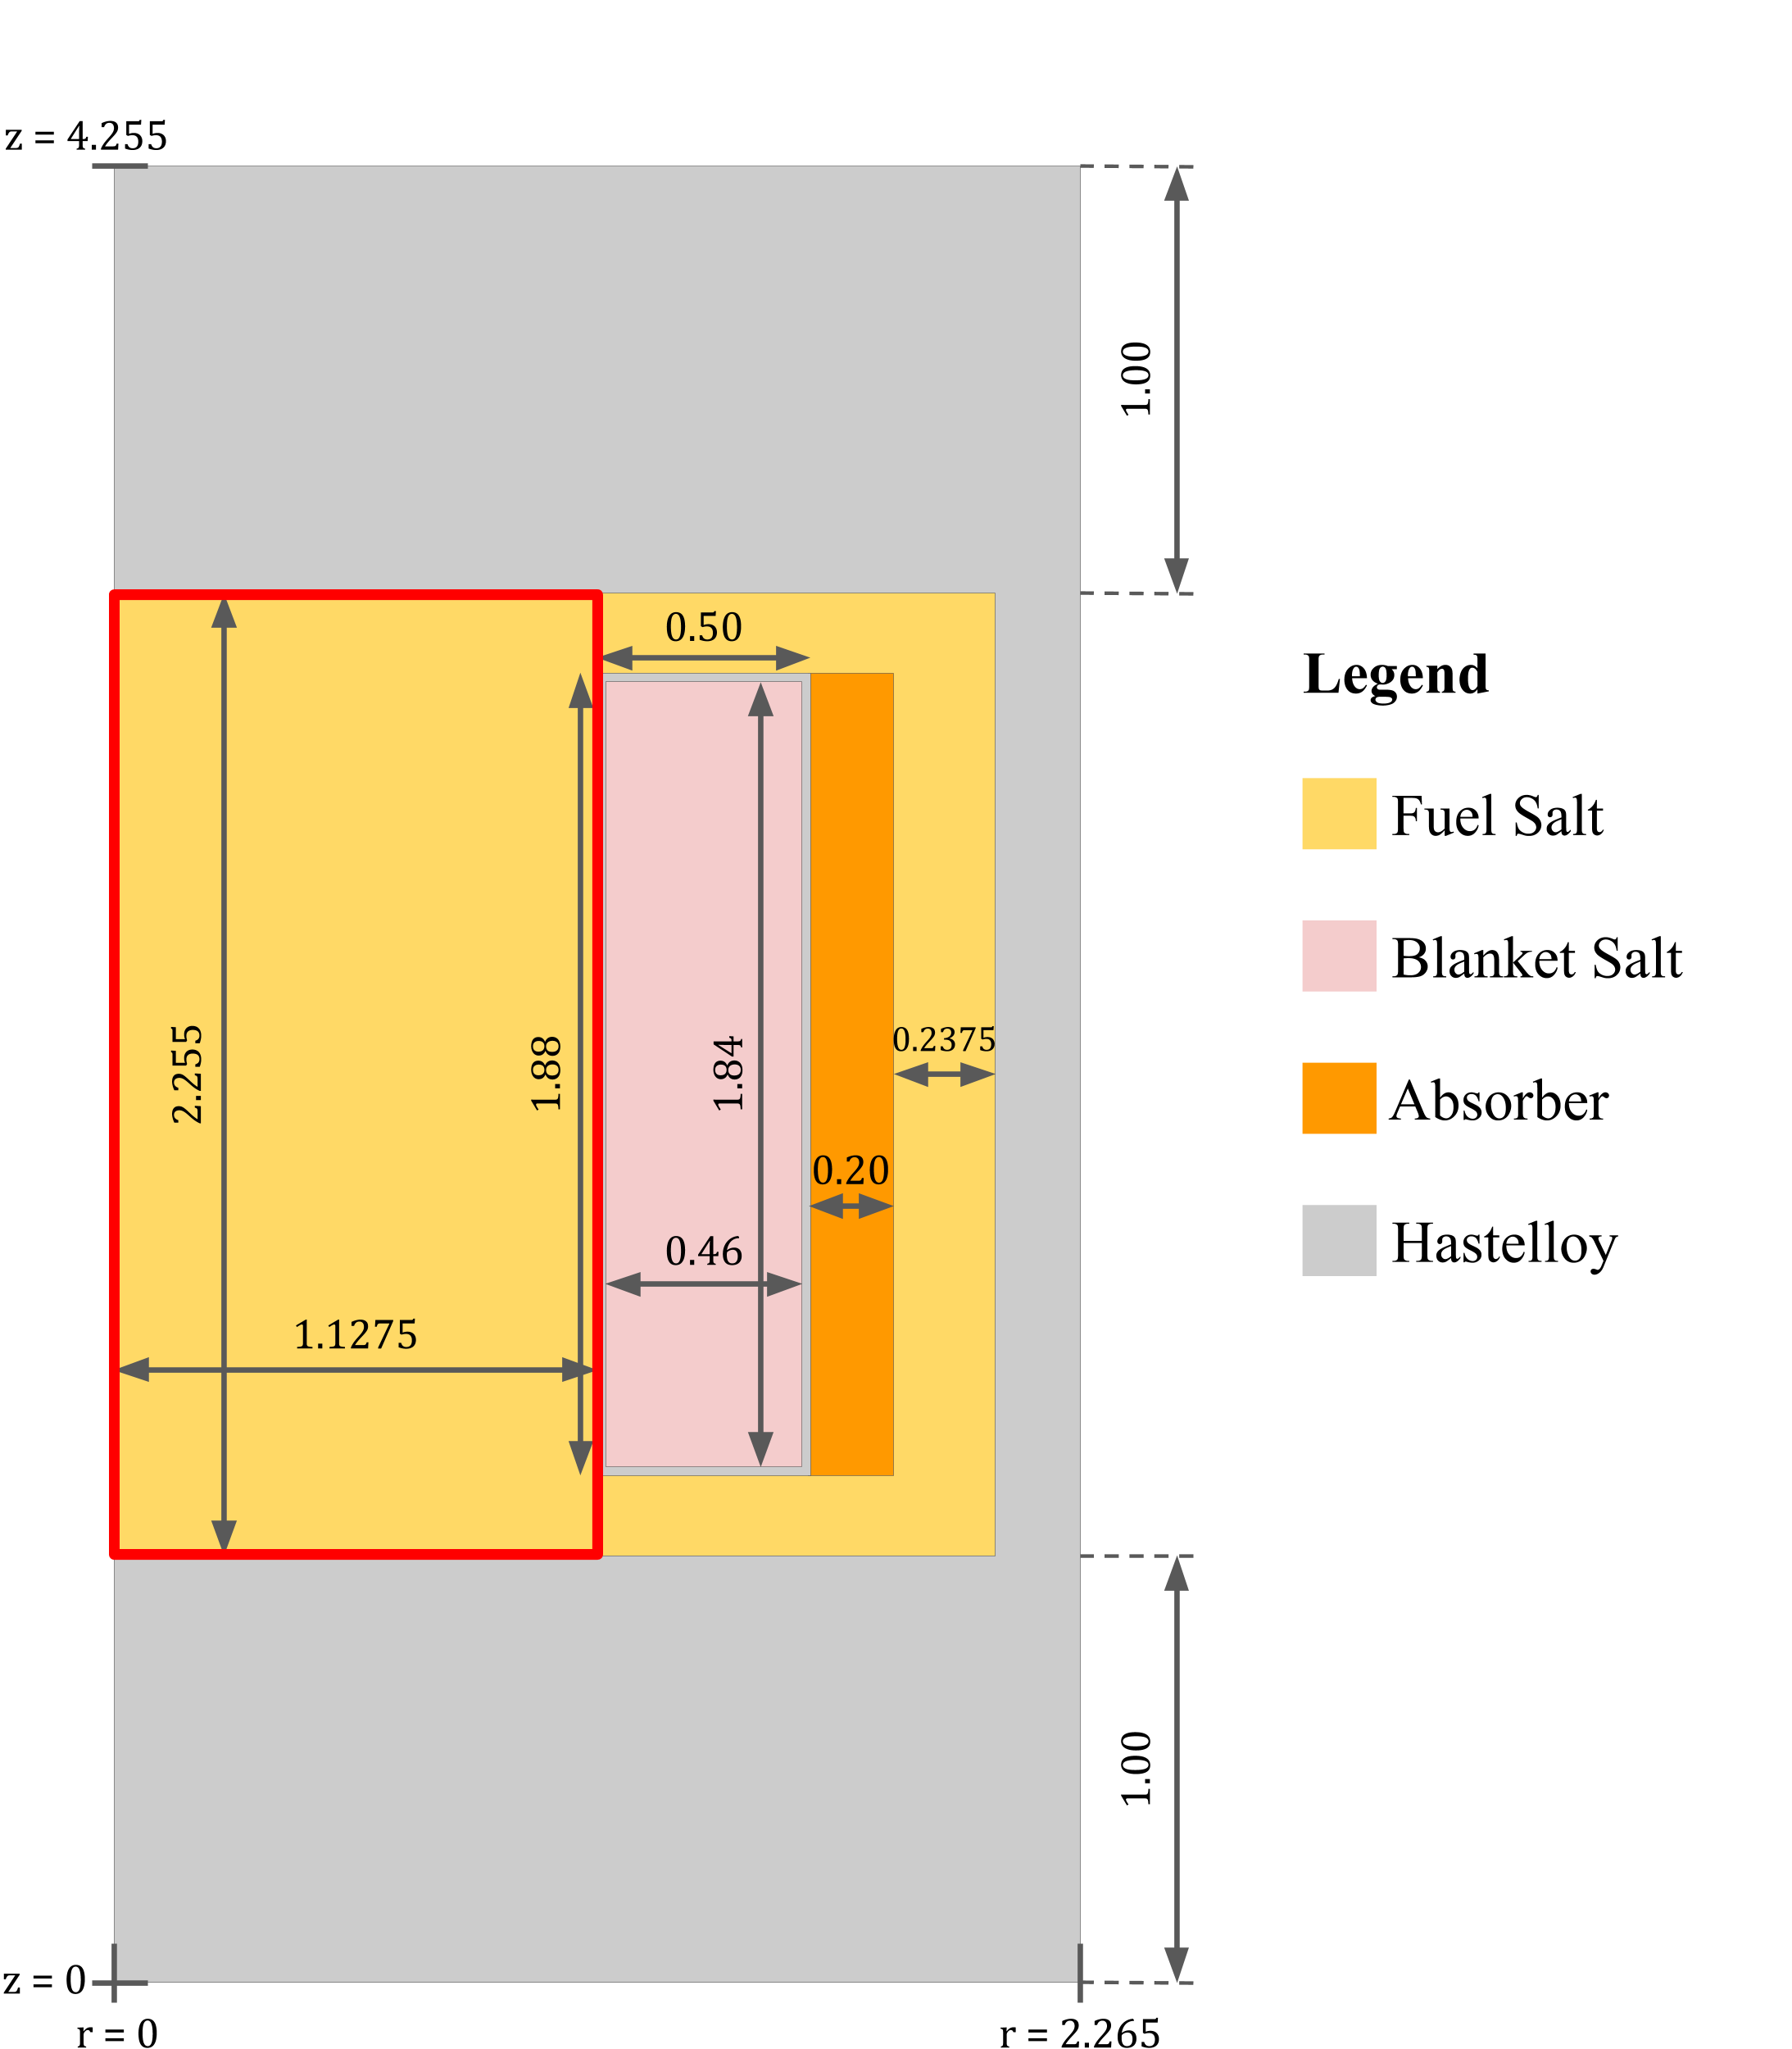
\includegraphics[width=.75\textwidth]{central-core-legend}
    \caption{2-D axisymmetric model of the MSFR. The red box indicates the
    central core region in the modeling approach in Moltres.}
    \label{fig:core}
\end{figure}

The central core region is of greatest interest to us during steady-state and
transient scenarios; the center of the reactor is naturally where most of the
fissions and heat generation occur.

\subsubsection{Neutronics Model}

Moltres performs neutron flux calculations in the central core region
using the standard formulations for the time-dependent multigroup
neutron diffusion equations and \gls{DNP} concentration equations as shown in
equations \ref{eq:neut} and \ref{eq:dnp}:
%
\begin{align}
    \frac{1}{v_g} \frac{\partial \phi_g}{\partial t} &= \nabla \cdot D_g
    \nabla \phi_g - \Sigma^r_g \phi_g +
    \sum^G_{g' \neq g} \Sigma^s_{g' \rightarrow g} \phi_{g'} + \chi^p_g
    \sum^G_{g'=1} (1-\beta) \nu \Sigma^f_{g'} \phi_{g'} + \chi^d_g \sum^I_i
    \lambda_i C_i, \label{eq:neut} \\
    \frac{\partial C_i}{\partial t} &= \beta_i \sum^G_{g'=1} \nu \Sigma^f_{g'}
    \phi_{g'} - \lambda_i C_i - \vec{u} \cdot \nabla C_i + \nabla \cdot
    K \nabla C_i, \label{eq:dnp} \\
    \intertext{where}
    v_g &= \text{average speed of neutrons in group $g$ [cm$\cdot$s$^{-1}$],} 
    \nonumber \\
    \phi_g &= \text{neutron flux in group $g$ [cm$^{-2}\cdot$s$^{-1}$],}
    \nonumber \\
    t &= \text{time [s],} \nonumber \\
    D_g &= \text{diffusion coefficient of neutrons in group $g$
    [cm$^2\cdot$s$^{-1}$],} \nonumber \\
    \Sigma^r_g &= \text{macroscopic cross section for removal of neutrons from
    group $g$ [cm$^{-1}$],} \nonumber \\
    \Sigma^s_{g' \rightarrow g} &= \text{macroscopic cross section of
    scattering from $g'$ to $g$ [cm$^{-1}$],} \nonumber \\
    \chi^p_g &= \text{prompt fission spectrum for neutrons in group $g$ [ - ],
    } \nonumber \\
    G &= \text{total number of discrete neutron groups [ - ],} \nonumber \\
    \nu &= \text{average number of neutrons produced per fission [ - ],}
    \nonumber \\
    \Sigma^f_{g} &= \text{macroscopic fission cross section for neutron in
    group $g$ [cm$^{-1}$],} \nonumber \\
    \chi^d_g &= \text{delayed fission spectrum for neutrons in group $g$
    [ - ],} \nonumber \\
    I &= \text{total number of delayed neutron precursor groups [ - ],}
    \nonumber \\
    \beta &= \text{total delayed neutron fraction [ - ],} \nonumber \\
    \beta_i &= \text{delayed neutron fraction of precursor group $i$ [ - ],}
    \nonumber \\
    \lambda_i &= \text{average decay constant of delayed neutron precursors in
    precursor group $i$ [s$^{-1}$],} \nonumber \\
    C_i &= \text{concentration of delayed neutron precursors in precursor
    group $i$ [cm$^{-3}$],} \nonumber \\
    K &= \text{turbulent diffusion coefficient of the delayed neutron
    precursors [cm$^2\cdot$s$^{-1}$].} \nonumber
\end{align}
%

While the limitations of the multigroup neutron diffusion method compared to
other deterministic and Monte Carlo methods, particularly for flux values near
boundaries, are well-documented, the diffusion model provides acceptable
accuracy at lower computational costs. Moreover, the central core region
contains no material interfaces except at its boundaries. Chapter
\ref{chap:nts} provides a comparison of the \gls{MSFR} multiplication factor
values and reactivity coefficients between Moltres and Serpent.

The \gls{DNP} concentration equation has additional advection and turbulent
diffusion terms to account for the movement of \glspl{DNP} in the primary
coolant loop. The turbulent diffusion $K$ is governed by the following
equation:
%
\begin{align}
    K &= \frac{\mu_t}{\rho Sc_t}
    \intertext{where}
    \mu_t &= \text{ eddy viscosity [Pa s],} \nonumber \\ 
    \rho &= \text{ density of the fuel salt [kg m$^{-3}$],} \nonumber \\
    Sc_t &= \text{ turbulent Schmidt number [ - ].} \nonumber
\end{align}
%
This work assumes $Sc_t = 0.85$ for a fair comparison with the Polimi and
TUDelft models \cite{fiorina_modelling_2014} which used the same value. It has
its roots in the Reynolds Analogy, which states that turbulent momentum and
heat transfer largely depend on the same eddies in turbulent flow
\cite{bartosiewicz_612_2019}. Therefore,
$Sc_t$ should be close to unity. $Sc_t = 0.85$ is also the default value for
most commercial \gls{CFD} software \cite{bartosiewicz_612_2019}.

\begin{figure}[htb!]
    \centering
    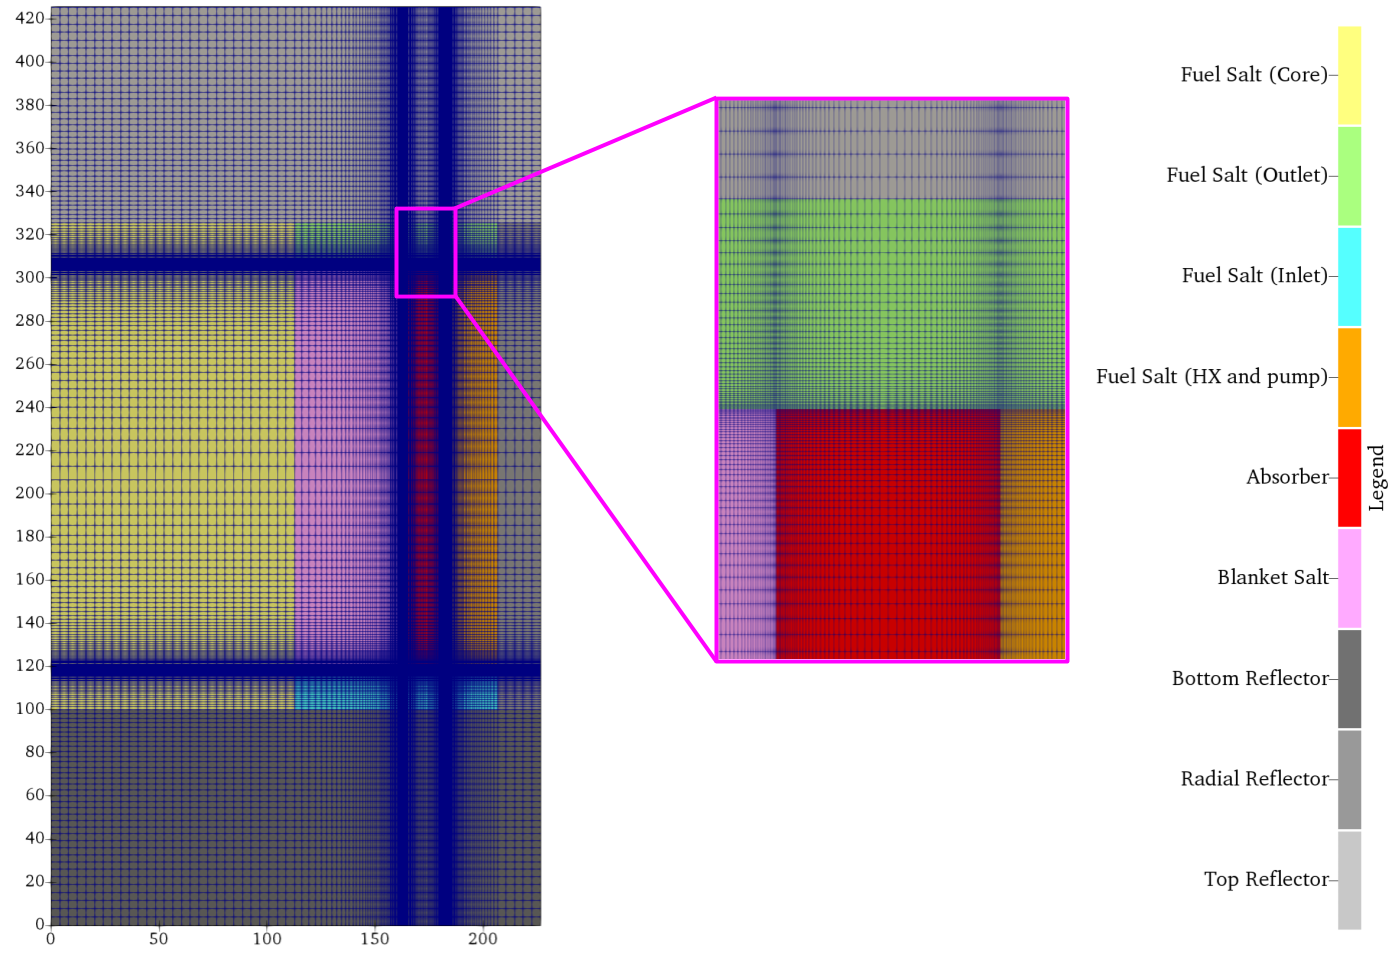
\includegraphics[width=\textwidth]{mesh2}
    \caption{Mesh adopted in Moltres and a close-up view of the mesh around
    the boron carbide absorber.}
    \label{fig:mesh}
\end{figure}

Moltres users can use an arbitrary number of neutron energy groups as
long as they provide Moltres with the appropriate group constant data. The
number of precursor groups is also variable, though usually predetermined by
the choice of nuclear data library in the group constant generation step.
Moltres automatically interpolates the group constant data for required
temperatures using one of the many predefined interpolation methods available
in \gls{MOOSE}. Once again, Moltres allows users to select their
interpolation method of choice.

This work uses six neutron energy groups according to the
energy boundaries in table \ref{table:bound}, and eight \gls{DNP} groups as
defined by the JEFF-3.1.2 library. The neutron flux
and \gls{DNP} concentration values were approximated by first-order Lagrange
and constant monomial shape functions respectively on the finite element mesh.
Figure \ref{fig:mesh} shows the mesh adopted for the \gls{MSFR} model.
This work assumes vacuum boundary conditions for all six neutron group fluxes
along the external boundaries of the geometry, and homogeneous Neumann
boundary conditions along the axial symmetry boundary. For the \gls{DNP}
concentrations, this work imposed homogeneous Neumann boundary conditions on
the walls, and inflow and outflow boundary conditions on the inlet and outlet
boundaries, respectively. The inlet \gls{DNP} concentration values were
imported from the outlet values of the 1-D outer loop pipe at the same
timestep. Table \ref{table:corebc} describes these boundary conditions
mathematically.

For the decay heat model, a previous study on the MSFR by Aufiero et al.
\cite{aufiero_extended_2013} showed that using three decay heat precursor
groups with appropriate half-lives in the form of exponential equations, can
accurately model decay heat in the MSFR for up to 300 seconds after shutdown
with a relative error of less than 2\%. Thus, this thesis implements the new
decay heat modeling capability with the following equation:
%
\pagebreak
\begin{align}
	\frac{\partial \omega_j}{\partial t} &= f_j \lambda_j \sum^G_{g=1}
	\epsilon_{g}
	\Sigma^f_{g} \phi_{g} - \lambda_j \omega_j - \vec{u} \cdot \nabla
	\omega_j + \nabla \cdot K \nabla \omega_j, \label{eq:decayheat} \\
	\intertext{where}
    \omega_j &= \text{total decay heat power density from decay heat
    precursors in group $j$ [W$\cdot$cm$^{-3}$],} \nonumber \\
	f_j &= \text{fraction of total power attributable to decay heat group
	$j$ [ - ],} \nonumber \\
	\epsilon_g &= \text{average fission energy per fission initiated by a
	neutron in group $g$ [W],} \nonumber \\
	\lambda_j &= \text{average decay constant of decay heat precursors in
	group $j$ [s$^{-1}$].} \nonumber
\end{align}

Like the neutron energy and \gls{DNP} groups, Moltres can accommodate an
arbitrary number of decay heat groups. The current work uses the same decay
heat fractions and decay constants, shown in Table \ref{eq:decayheat}, used in
the Polimi and TUDelft models for three decay heat groups.

\begin{table}[htb!]
	\centering
	\caption{Decay heat group parameters \cite{fiorina_modelling_2014}.}
	\begin{tabular}{S S S}
		\toprule
		{Decay heat group $j$} & {$\lambda_j$ [s$^{-1}$]} & {$f_j$} \\
		\midrule
		1 & 0.1974 & 0.0117 \\
		2 & 0.0168 & 0.0129 \\
		3 & 0.000358 & 0.0186 \\
		\bottomrule
	\end{tabular}
	\label{table:decayheat}
\end{table}

\subsubsection{Thermal-Hydraulics Model}

This work models fluid dynamics using the \gls{INS} capabilities from the
MOOSE Navier-Stokes module \cite{peterson_overview_2017}. The standard
\gls{INS} equations are:
%
\begin{align}
    \text{Momentum eq.:} && \rho \frac{\partial \vec{u}}{\partial t} &=
    -\rho (\vec{u}
    \cdot \nabla) \vec{u} + \nabla \cdot [-p \vec{I} + \mu [
    \nabla \vec{u} + (\nabla \vec{u})^T]] + \vec{f} &&
    \label{eq:momemtum} \\
    \text{Divergence-free:} && \nabla \cdot \vec{u} &= 0 &&
    \label{eq:divergence}
    \intertext{where}
    && p &= \text{ pressure [Pa],} && \nonumber \\
    && \mu &= \text{ dynamic viscosity [Pa$\cdot$s],} && \nonumber \\
    && \vec{f} &= \text{ body force per unit volume [N$\cdot$m$^{-3}$].} &&
    \nonumber
\end{align}

In addition to the intrinsic molecular viscosity in the \gls{INS} equations,
this thesis includes an eddy viscosity term, $\mu_t$, to approximate
turbulent flow effects. The current implementation of the Navier-Stokes module
does not have a turbulence model. The options for turbulence modeling in
\gls{CFD} include direct numerical simulations (DNS) and large eddy
simulations (LES) for higher fidelity flow simulations, \gls{RANS} methods for
balanced compromises between accuracy and computational speed, and lumped
parameter and sub-channel methods for even faster performance with greater
accuracy costs \cite{moorthi_review_2018}. The Polimi and TUDelft models used
\gls{RANS} methods to model salt flow \cite{fiorina_modelling_2014}. This work
uses a zeroth-order approximation of $\mu_t$ based on the calculated $\mu_t$
values reported in the Polimi and TUDelft models. The models predicted spatial
$\mu_t$ values ranging from 0 to 110 Pa$\cdot$s, with most values
falling within the 30 to 50 Pa$\cdot$s range. Thus, the present work uses
the approximated value $\mu_t=$ 40 Pa$\cdot$s. Despite the simplicity of this
approximation, the resulting flow profile is similar to the flow profile in
the Polimi and TUDelft models at steady-state.

The energy balance equation for temperature used in this Moltres model is:
%
\begin{align}
    \rho c_{p} \frac{\partial T}{\partial t} &= - \rho c_p \vec{u}
    \cdot \nabla T + \nabla \cdot [(k + k_t) \nabla T] + Q_s
    \label{eq:temp} \\
    k_t &= \frac{\mu_t}{\rho Pr_t} \\
    Q_s &= \Big( 1 - \sum^J_{j=1} f_j \Big) \sum^G_{g=1} \epsilon_g \Sigma_g^f
    \phi_g + \sum^J_{j=1} \omega_j, \label{eq:source}
    \intertext{where}
    c_p &= \text{specific heat capacity of molten salt
    [J$\cdot$kg$^{-1}\cdot$K$^{-1}$],} \nonumber \\
    T &= \text{temperature of molten salt [K]} \nonumber \\
    \vec{u} &= \text{velocity of molten salt [m$\cdot$s$^{-1}$],}
    \nonumber \\
    k &= \text{thermal conductivity of molten salt
    [W$\cdot$m$^{-1}\cdot$K$^{-1}$],} \nonumber \\
    J &= \text{total number of decay heat groups [ - ].} \nonumber
\end{align}
%
The diffusion term includes turbulent heat
diffusivity based on the eddy viscosity $\mu_t$ and the turbulent Prandtl
number $Pr_t$. $Pr_t$ is also 0.85 due to the same reasoning provided for
$Sc_t$. The first term in the heat source $Q_s$ equation represents prompt
fission heat, and the second term represents decay heat from the $J$ decay
heat groups.

With this model, the results were expected to show good qualitative agreement
with the Polimi and TUDelft models, including the large recirculation region
near the blanket tank walls and the resulting high temperatures in that
region. The results in Chapter \ref{chap:ss} show minor discrepancies in
regions where the viscosity values were under- or over-predicted.

\subsubsection{Boundary Conditions}

Table \ref{table:corebc} summarizes the boundary conditions for all variables
on all of the relevant boundaries. Figure \ref{fig:msfrbc} shows the locations
of the various boundaries listed in the table. The CoupledOutflow boundary
condition for $C_i$ and $\omega_j$ is a new feature in Moltres that allows
users to couple these variables to the outlet velocity components (e.g. $u_x$,
$u_y$). Without this boundary condition, users could only use uniform or fixed
function-based velocity profiles in conjunction with the precursor looping
capability.

\begin{table}[htbp!]
    \small
	\caption{Boundary conditions in the main reactor geometry (Figure
	\ref{fig:msfrbc}).}
	\centering
	\begin{tabular}{ l l c}
		\toprule
		Variable & Boundary & Boundary Condition \\
		\midrule
		\multirow{4}{*}{Neutron flux $\phi_g$} & Top & $\frac{d \phi_g}{dx}
		\big|_{\text{inflow}} = 0$ \\[.5ex]
        & Outer & $\frac{d \phi_g}{dx} \big|_{\text{inflow}} = 0$ \\[.5ex]
        & Bottom & $\frac{d \phi_g}{dx} \big|_{\text{inflow}} = 0$ \\[.5ex]
        & Axial & $\frac{d \phi_g}{dx} = 0$ \\[.5ex]
        \midrule
        \multirow{6}{*}{Delayed neutron precursor concentration $C_i$} &
        Top (Core) & $\frac{d C_i}{dx} = 0$ \\[.5ex]
        & Bottom (Core) & $\frac{d C_i}{dx} = 0$ \\[.5ex]
        & Outer (Core) & $\frac{d C_i}{dx} = 0$ \\[.5ex]
        & Axial (Core) & $\frac{d C_i}{dx} = 0$ \\[.5ex]
        & Inlet (Core) & $C_i = c$ \\
        & Outlet (Core) & $u_x \cdot C_i = 0$ \\
        \midrule
        \multirow{6}{*}{Decay heat power density $\omega_j$} &
        Top (Core) & $\frac{d \omega_j}{dx} = 0$ \\[.5ex]
        & Bottom (Core) & $\frac{d \omega_j}{dx} = 0$ \\[.5ex]
        & Outer (Core) & $\frac{d \omega_j}{dx} = 0$ \\[.5ex]
        & Axial (Core) & $\frac{d \omega_j}{dx} = 0$ \\[.5ex]
        & Inlet (Core) & $\omega_j = c$ \\
        & Outlet (Core) & $u_x \cdot \omega_j = 0$ \\
        \midrule
        \multirow{6}{*}{Radial velocity $u_x$} & Top (Core) & $u_x = 0$ \\
        & Bottom (Core) & $u_x = 0$ \\
        & Outer (Core) & $u_x = 0$ \\
        & Axial (Core) & $u_x = 0$ \\
        & Inlet (Core) & $u_x = c$ \\
        & Outlet (Core) & $\frac{d u_x}{dx} = 0$ \\[.5ex]
        \midrule
        \multirow{6}{*}{Axial velocity $u_y$} & Top (Core) & $u_y = 0$ \\
        & Bottom (Core) & $u_y = 0$ \\
        & Outer (Core) & $u_y = 0$ \\
        & Axial (Core) & $\frac{d u_y}{dx} = 0$ \\[.5ex]
        & Inlet (Core) & $u_y = 0$ \\
        & Outlet (Core) & $\frac{d u_y}{dx} = 0$ \\[.5ex]
        \midrule
        \multirow{6}{*}{Temperature $T$} & Top (Core) &
        $\frac{d T}{dx} = 0$ \\[.5ex]
        & Bottom (Core) & $\frac{d T}{dx} = 0$ \\[.5ex]
        & Outer (Core) & $\frac{d T}{dx} = 0$ \\[.5ex]
        & Axial (Core) & $\frac{d T}{dx} = 0$ \\[.5ex]
        & Inlet (Core) & $T = c$ \\
        & Outlet (Core) & $\frac{d T}{dx} = 0$ \\[.5ex]
		\bottomrule
	\end{tabular}
	\label{table:corebc}
\end{table}

\clearpage

\begin{figure}[htb!]
    \centering
    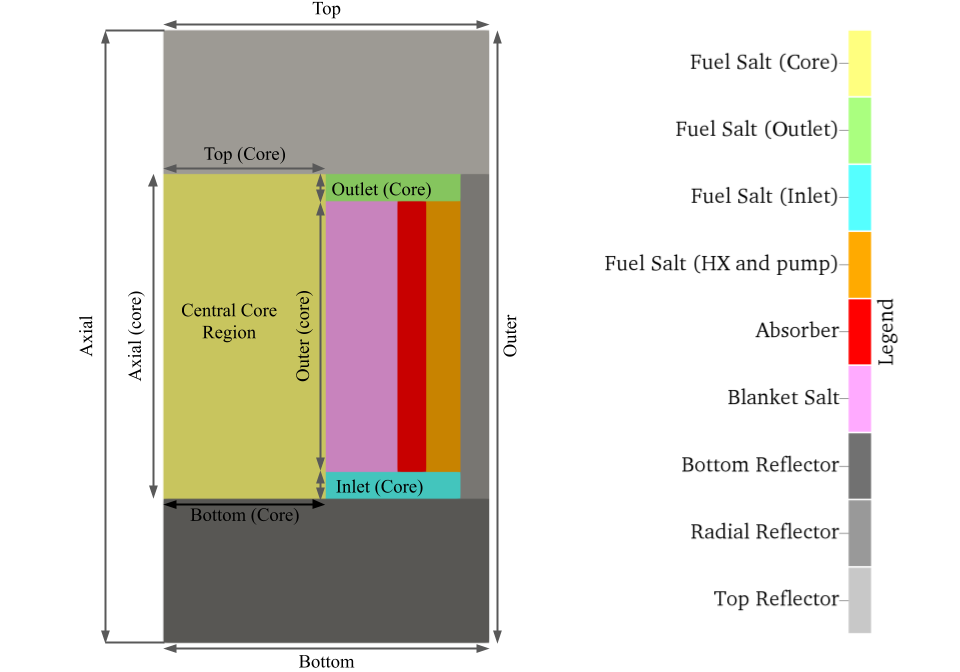
\includegraphics[width=.8\textwidth]{msfrbc}
    \caption{The boundaries in the \gls{MSFR} geometry that are relevant for
    the boundary conditions mentioned in Table \ref{table:corebc}.}
    \label{fig:msfrbc}
\end{figure}

\subsection{Outer Loop Region}

Moltres also accounts for the decay of
\glspl{DNP} outside the central core region by simulating its flow in a
separate 1-D pipe geometry. This outer loop pipe calculation is implicitly
coupled to the active core simulation through Picard iterations in MOOSE's
MultiApp functionality and inlet/outlet boundary values. For this work with
the \gls{MSFR} model, the pipe length is 2.255 m with salt flowing at 1.1275 m
s$^{-1}$ for an out-of-core residence time of 2 s. The present author derived
these parameters from the reference specifications of 4s cycle
time and 50\% out-of-core salt fraction (Table \ref{table:msfr}).

\subsubsection{Neutronics Model}

The outer loop region is largely subcritical because most of it is adjacent to
the boron carbide absorber as shown in Figure \ref{fig:core}. Therefore, the
only significant neutronics-related phenomena are the drift and decay of
\glspl{DNP}. The governing equation for the \glspl{DNP} is:
%
\begin{align}
    \frac{\partial C_i}{\partial t} &= - \lambda_i C_i - u
    \frac{\partial C_i}{\partial x}.
    \label{eq:dnploop}
\end{align}
%
Equation \ref{eq:dnploop} is derived from equation \ref{eq:dnp} by removing
the fission \gls{DNP} source term, and the conversion of the advection and
diffusion terms to their 1-D forms. The decay constants and diffusion
coefficient are the same values used in the central core region.

\subsubsection{Thermal-Hydraulics Model}

A constant velocity of 1.1275 m s$^{-1}$ is applied in the outer loop region
to maintain the nominal 2s out-of-core residence time. The governing equation
for temperature, derived from equation \ref{eq:temp}, is:
%
\begin{align}
    \rho c_{p} \frac{\partial T}{\partial t} &= - \rho c_p u
    \frac{\partial T}{\partial x} - Q_{hx} \label{eq:temploop} \\
    Q_{hx} &= \alpha (T - T_i) \delta (x_0) \label{eq:hx} \\
    \intertext{where}
    Q_{hx} &= \text{heat removal rate through the heat exchanger [W],} 
    \nonumber \\
    \alpha &= \text{heat transfer coefficient [W$\cdot$K$^{-1}$],} \nonumber
    \\
    T_i &= \text{temperature of the intermediate salt [K],} \nonumber \\
    x_0 &= \text{position of the point heat exchanger [m].} \nonumber
\end{align}

In the outer loop region, the fission heat source term is replaced with a heat
exchanger sink term $Q_{hx}$
which depends on the temperature difference between the fuel salt $T$ and the
intermediate loop salt $T_i$. For simplicity, this work assumes a constant
temperature of 823 K in the intermediate loop. The heat transfer coefficient
was determined by assuming that the fuel outlet temperature is 1023 K and
calculating the heat removal rate to induce a 100 K drop at the given
volumetric flow rate and heat capacity of the fuel salt. The resulting value
for $\alpha$ is 370.668 W$\cdot$K$^{-1}$. This work opted to
ignore the diffusion term due to the discontinuity of the temperature
distribution across the point heat exchanger. 

\subsubsection{Boundary Conditions}

Table \ref{table:loopbc} summarizes the boundary conditions for all variables
on the inlet and outlet of the 1-D outer loop region. The inlet boundary
conditions are all Dirichlet boundary conditions. The inlet boundary values
are set by the outflow from the central core region that this inlet is
connected to in the actual reactor geometry. The outlet boundary conditions
are all outflow boundary conditions as shown in Table \ref{table:loopbc}.

\begin{table}[htbp!]
    \small
	\caption{Boundary conditions in the 1-D outer loop geometry. $u$
	represents the 1-D velocity in this region.}
	\centering
	\begin{tabular}{ l l c}
		\toprule
		Variable & Boundary & Boundary Condition \\
        \midrule
        \multirow{2}{*}{Delayed neutron precursor concentration $C_i$} &
        Inlet (Core) & $C_i = c$ \\
        & Outlet (Core) & $u \cdot C_i = 0$ \\
        \midrule
        \multirow{2}{*}{Decay heat power density $\omega_j$} &
        Inlet (Core) & $\omega_j = c$ \\
        & Outlet (Core) & $u \cdot \omega_j = 0$ \\
        \midrule
        \multirow{2}{*}{Temperature $T$} &
        Inlet (Core) & $T = c$ \\
        & Outlet (Core) & $u \cdot T = 0$ \\
		\bottomrule
	\end{tabular}
	\label{table:loopbc}
\end{table}

\subsection{Central Core and Outer Loop Coupling}

This subsection details the delayed neutron and decay heat precursors, and
temperature coupling between the central core and outer loop regions. 

%Starting with the central core region, for the neutron group fluxes, we
%imposed vacuum boundary conditions on the
%outermost boundaries of the geometry in Figure \ref{fig:core} excluding the
%axial boundary. The \gls{DNP} variables have homogeneous Neumann boundary
%conditions along the axis and the walls in the central core region, and inflow
%and outflow boundary conditions on the inlet and outlet boundaries,
%respectively. The temperature variable shares the same type of boundary
%conditions as the \gls{DNP} variables.

This work uses a parabolic flow profile on the inlet Dirichlet boundary
condition. The equation for $u_x$ at the inlet is:
%
\begin{align}
    u_x &= -\xi \Big[\frac{y}{H} - \Big(\frac{y}{H}\Big)^2 
    \Big] \\
    \intertext{where}
    \xi &= \text{normalizing constant [m$\cdot$s$^{-1}$],} \nonumber \\
    y &= \text{height along the inlet [m],} \nonumber \\
    H &= \text{total height of the inlet $= 0.1875$ m.} \nonumber
\end{align}
%
$\xi$ is a normalizing constant that depends on the total volumetric flow
rate, $\dot{V}$. Solving the following set of equations in $v$ and $\dot{V}$:
%
\begin{align}
    v &= \xi [\frac{y}{H} - \frac{y^2}{H^2}] \\
    \dot{V} &= \int^h_0 \int^{2 \pi}_0 v r d\theta dy \\
    \intertext{where}
    r &= \text{radius [m],} \nonumber \\
    \theta &= \text{azimuthal angle [rad],} \nonumber
\end{align}
%
gives $\xi = 20.3401$ m$\cdot$s$^{-1}$ for $\dot{V} = 4.5$ m$^3\cdot$s$^{-1}$. 

At every timestep, Moltres also calculates weighted averages of the
temperature and the precursors at the outlet. These values are weighted by the
outflow velocity values at the outlet according to the following equation:
%
\begin{align}
    \overline{\psi} &= \frac{\int_\mathcal{C} \psi(y) u(y) dy}{
    \int_\mathcal{C} u(y) dy} \\
    \intertext{where}
    \psi &= \text{variable to be weighted [ - ]} \nonumber \\
    \mathcal{C} &= \text{outlet boundary area [ - ]} \nonumber \\
    u &= \text{outflow velocity perpendicular to the outlet boundary
    [m$\cdot$s$^{-1}$].} \nonumber
\end{align}

Moltres transfers this outflow value from the central core region to the 1-D
outer loop region, to be used as the boundary value for the inhomogeneous
Dirichlet boundary
condition at the inlet. Likewise, the outflow value from the outer
loop region is used for the inflow value in the central core region. No
averaging is required for this step as the outer loop region is a 1-D system.
We assume that the inflow temperature and \gls{DNP} are uniform at the inlet.
The Picard iterations within every timestep ensure that the two systems are
implicitly coupled even though they're solved separately.


\chapter{Neutronics Assessment}
This chapter verifies Moltres' ability to reproduce key neutronics parameters
using group constant data from Serpent 2, which is essential for accurate
neutronics calculations in the subsequent multiphysics simulations. The model
under study is a static model of the \gls{MSFR}, i.e. no salt flow, and
uniform temperature distribution to assess the accuracy of the
six-group neutron diffusion model in Moltres on a fast-spectrum reactor. Table
\ref{table:static} lists relevant details of the static \gls{MSFR} model
in Moltres. This
verification exercise builds on the previous study by Lindsay et al.
\cite{lindsay_introduction_2018} that verified Moltres' neutronics
capabilities with a two-group neutron diffusion model of the \gls{MSRE}.

\begin{table}[htbp!]
    \small
	\caption{Details of the static \gls{MSFR} model in Moltres.}
	\centering
	\begin{tabular}{ l c}
		\toprule
		Detail & Mathematical description \\
        \midrule
        No salt flow (static salt) & $v_{salt} = 0$ m$\cdot$s$^{-1}$ \\
        Uniform temperature of 973 K throughout the 2D core model & $T = 973$
        K \\
        Six neutron energy groups & $G = 6$ \\
        Eight delayed neutron precursor groups & $I = 8$ \\
        Vacuum boundary conditions for neutron flux &
        $\frac{d \phi}{dx}\big|_{\text{inflow}} = 0$ m$^{-2}\cdot$s$^{-1}$ \\
		\bottomrule
	\end{tabular}
	\label{table:static}
\end{table}

\section{Effective Multiplication Factor and Delayed Neutron Fraction}

Moltres solves the six-group neutron diffusion equations (Equation
\ref{eq:neut}) as a
steady-state eigenvalue problem to find the $k_{\text{eff}}$ for the static
\gls{MSFR} model. Table
\ref{table:keff} shows the $k_{\text{eff}}$ values from Serpent 2 and Moltres
at 973 K and the corresponding salt density, and Table \ref{table:ktemp} shows
the $k_{\text{eff}}$ values for other temperatures at 100 K intervals. Two
main factors contribute to the small discrepancies on the order of 100 pcm
between the two applications: the accuracy of the neutron diffusion
model, and the omission of the blanket tank structural material in Moltres.
The neutron diffusion model is not as accurate as the other S$_{\text{N}}$ or
SP$_{\text{N}}$ deterministic methods nor the Monte Carlo approach in Serpent.
Regarding the omission of the blanket tank material, I
replaced the 2 cm-thick structural material with blanket salt. This
replacement is partly responsible for the higher $k_{\text{eff}}$ value
calculated by Moltres as fissions occur in the blanket salt. Nevertheless, the
discrepancy is smaller
than the 228.5 pcm and 256.7 pcm discrepancies reported by Cervi et al.
\cite{cervi_development_2019} for their six-group $SP_3$ and neutron
diffusion methods, respectively.

\begin{table}[htb!]
    \small
	\centering
	\caption{$k_{\text{eff}}$ values from Serpent 2 and Moltres at 973 K.}
	\begin{tabular}{l S c}
		\toprule
		{Code} & {$k_{\text{eff}}$} \\
		\midrule
		{Serpent 2} & 1.00662 \pm 0.00005 \\
		{Moltres with \glspl{DNP}} & 1.0079400 \pm 0.0000010 \\
		{Moltres without \glspl{DNP}} & 1.0049197 \pm 0.0000010 \\
		\bottomrule
	\end{tabular}
	\label{table:keff}
\end{table}
%
\begin{table}[htb!]
    \small
	\centering
	\caption{$k_{\text{eff}}$ values from Serpent 2 and Moltres at various
	temperatures from 800 K to 1400 K.}
	\begin{tabular}{S S S S}
		\toprule
		{Temperature [K]} & {$k_{\text{eff}}$ $\pm$ $\sigma$
		(Serpent 2)} & {$k_{\text{eff}}$ (Moltres)} & {Difference wrt Serpent
		2 [pcm]}
		\\
		\midrule
		800  & 1.01996 \pm 0.00005 & 1.02117 & 121 \\
		900  & 1.01172 \pm 0.00005 & 1.01322 & 150 \\
		1000 & 1.00428 \pm 0.00005 & 1.00544 & 116 \\
		1100 & 0.99735 \pm 0.00005 & 0.99859 & 124 \\
		1200 & 0.99006 \pm 0.00005 & 0.99119 & 113 \\
		1300 & 0.98356 \pm 0.00005 & 0.98439 &  83 \\
		1400 & 0.97702 \pm 0.00005 & 0.97820 & 118 \\
		\bottomrule
	\end{tabular}
	\label{table:ktemp}
\end{table}

The absolute value of $k_{\text{eff}}$ impacts the final steady-state
temperature of the reactor. We can raise or lower the average core temperature
at steady state to meet the design specifications for the inlet and outlet
temperatures by adjusting the fissile inventory. On the other hand, the
delayed neutron fraction, $\beta$, and reactivity coefficients, $\alpha$, are
clearer indicators of transient reactor behavior in an accident transient.
$\beta$ primarily affects the magnitude of the initial change in power and the
time delay towards the new equilibrium power, while $\alpha$ affects the
magnitude of the change in reactor power and temperature.

This work compares the $\beta$ value from Moltres to the
$\beta_{\text{eff}}$ value from Serpent because Moltres currently lacks an
adjoint calculation capability.
The difference between $\beta$ and $\beta_{\text{eff}}$ is
that $\beta$ is the unweighted delayed neutron fraction
while $\beta_{\text{eff}}$ is the delayed neutron fraction weighted by the
adjoint neutron flux. I calculated $\beta$ by
taking the relative difference between the $k_{\text{eff}}$ values with and
without \glspl{DNP} in Table \ref{table:keff}. The $\beta$ and
$\beta_{\text{eff}}$ values at 973 K, shown in Table \ref{table:betaeff}, are
in good agreement with a 4.43 pcm discrepancy.

\begin{table}[htb!]
	\centering
	\caption{$\beta_{\text{eff}}$ and $\beta$ values from Serpent 2 and
	Moltres, respectively, at 973 K.}
	\begin{tabular}{l S S}
		\toprule
		{Code} & {$\beta_{\text{eff}}$ [pcm]} & {Difference wrt Serpent [pcm]}
		\\
		\midrule
		{Serpent} & 304.08 \pm .81 & {-}\\
		{Moltres} & 299.65 \pm .20 & 4.43\\
		\bottomrule
	\end{tabular}
	\label{table:betaeff}
\end{table}

\section{Reactivity Feedback Coefficients}

Temperature reactivity feedback arises mainly from Doppler broadening of
resonance absorption peaks and thermal expansion. The current work reports
the reactivity, $\rho$, values for temperatures from 800 K to 1400 K at 100 K
intervals (Figure \ref{fig:reactivity}). The slopes represent the total,
Doppler, density $\alpha$ values. The temperature range
extends below the melting point of the fuel salt (841 K) to ensure that
the data covers the relevant range between 841 K and 900 K. Table
\ref{table:alpha} shows the various $\alpha$ values calculated using the
linear least squares approach. The total temperature
coefficients from Serpent and Moltres show excellent agreement with a
discrepancy of 0.019 pcm K$^{-1}$.

\begin{figure}[htb!]
    \centering
    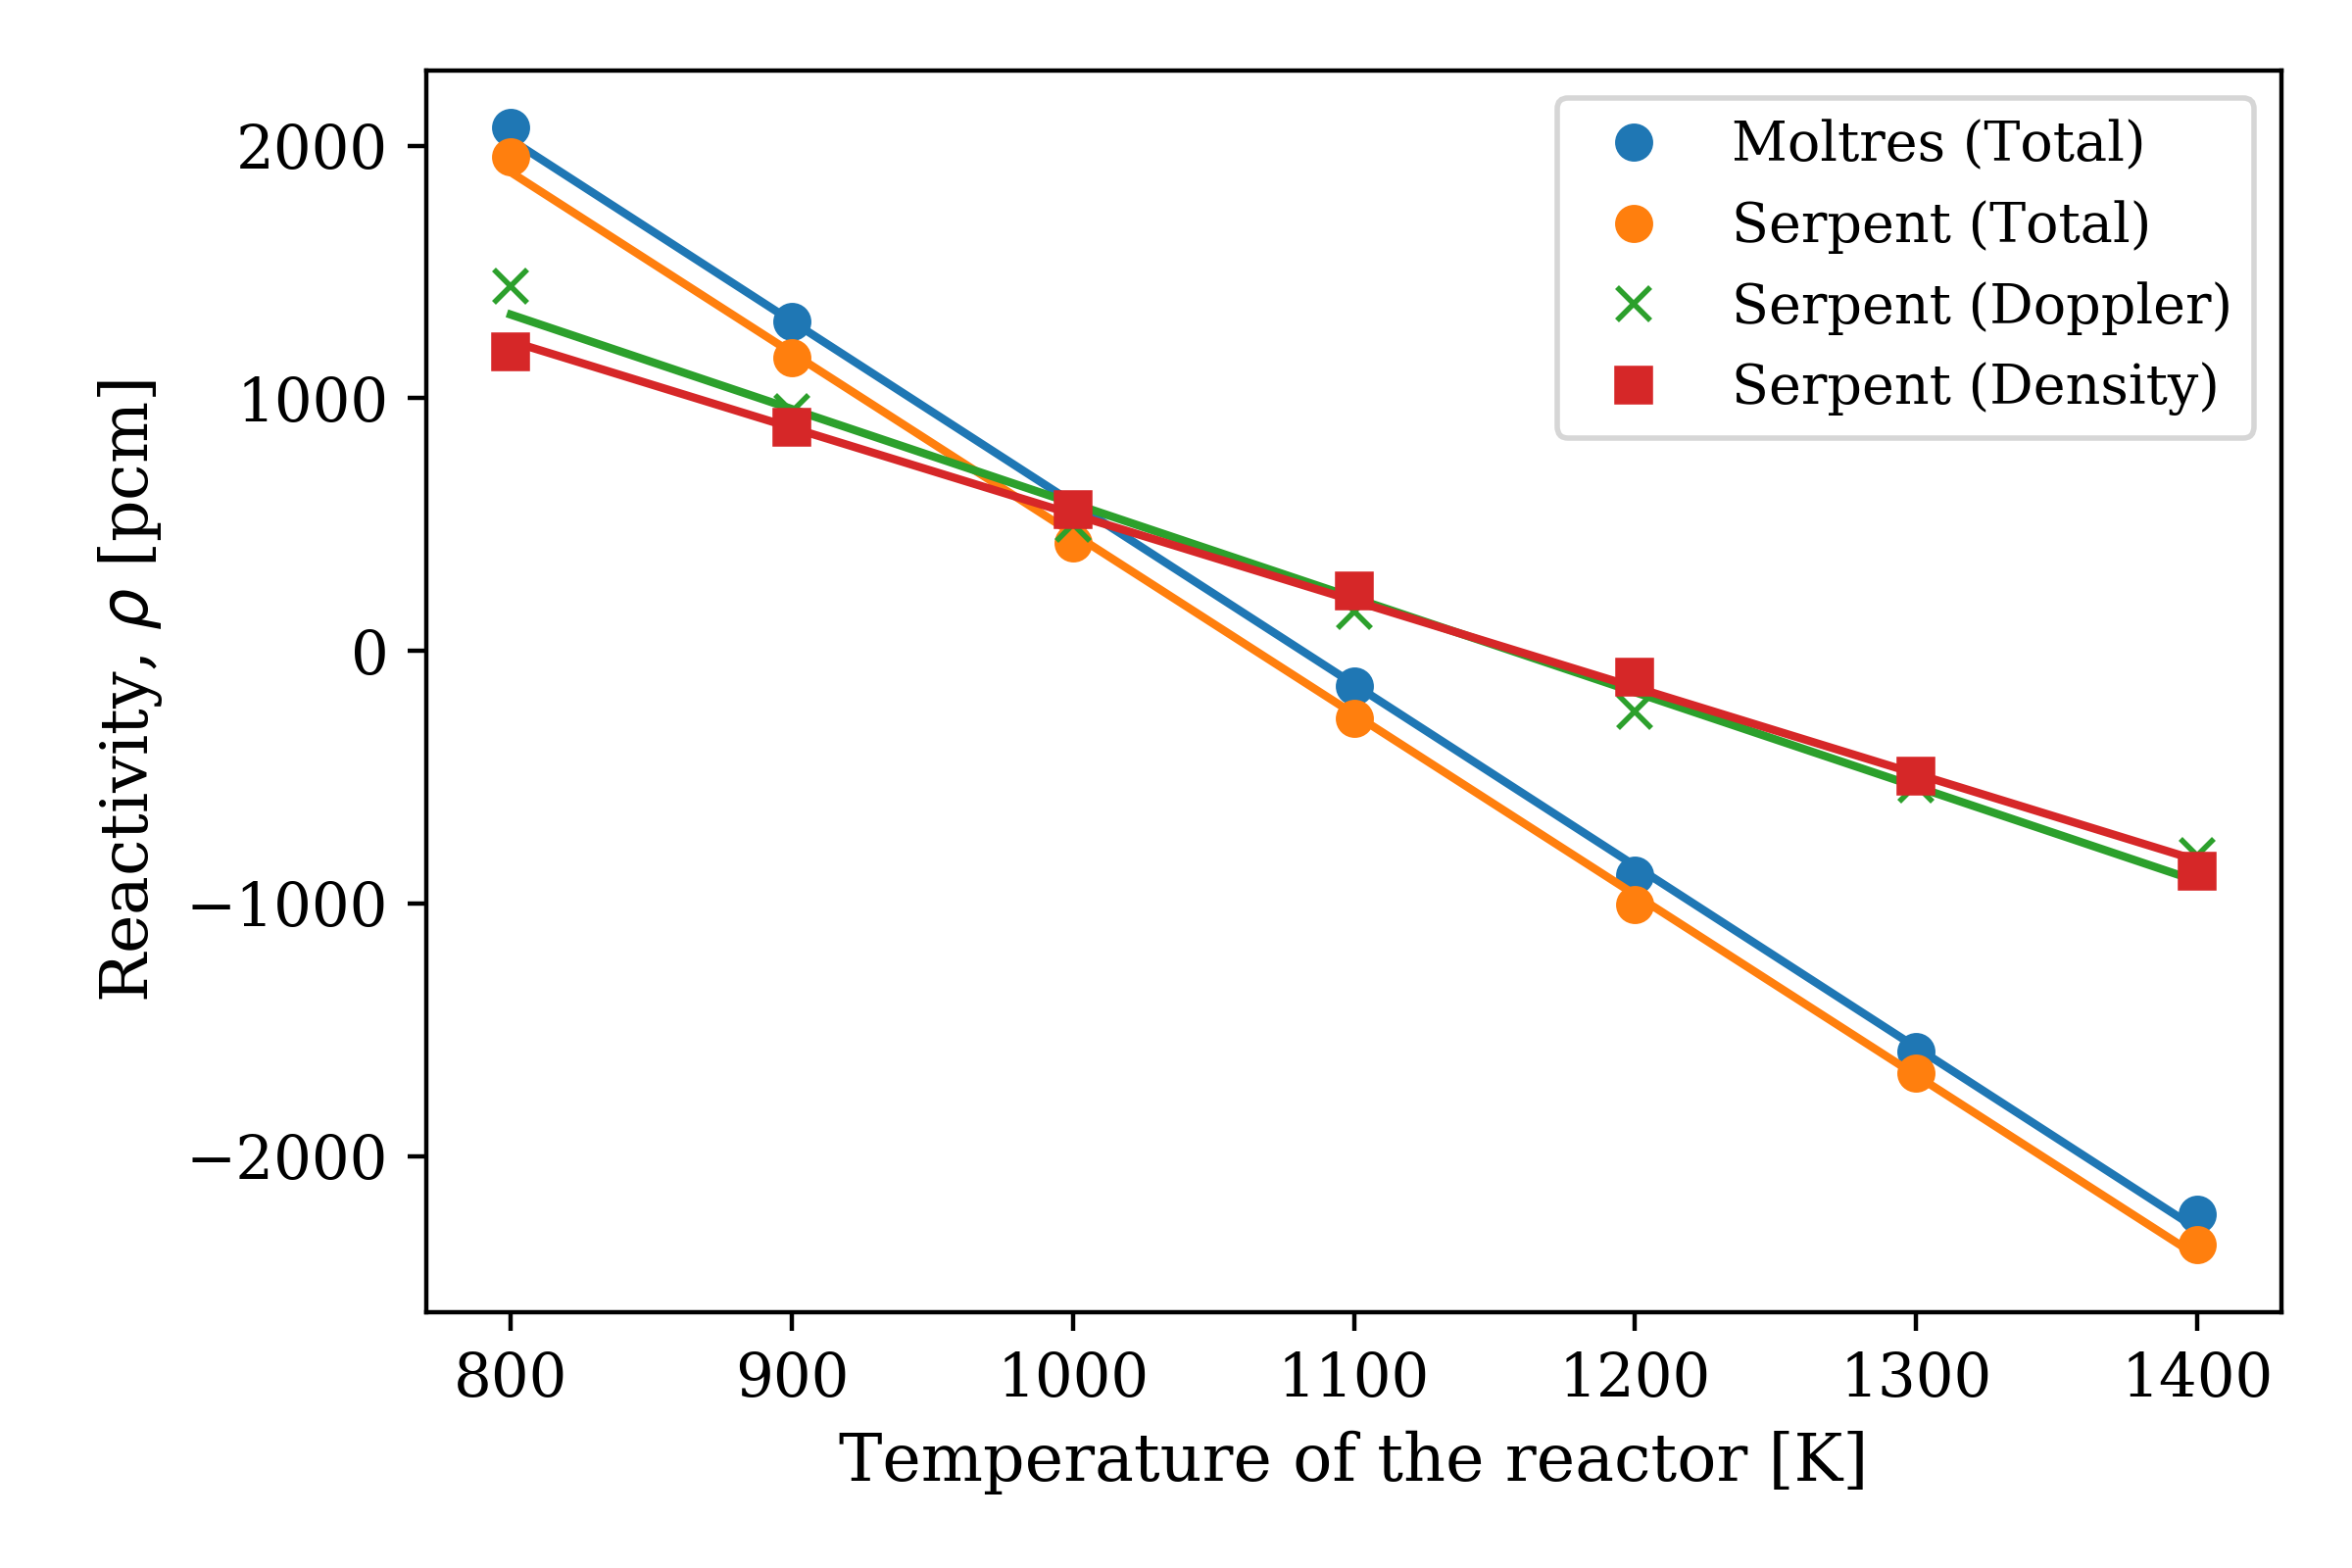
\includegraphics[width=.8\textwidth]{reactivity}
    \caption{Reactivity values from Serpent and Moltres. The Doppler
    reactivity values were calculated at a fixed density of 4.1249 g
    cm$^{-3}$. The thermal expansion reactivity values were calculated at a
    fixed temperature of 973 K.}
    \label{fig:reactivity}
\end{figure}
%
\begin{table}[htb!]
	\centering
	\caption{Doppler, density, and total temperature coefficients
	for the temperature range of 800 K to 1400 K.}
	\begin{tabular}{l S S S}
		\toprule
		{Software} & {$\alpha_D$ [pcm
		K$^{-1}$]} & {$\alpha_\rho$ [pcm K$^{-1}$]} & {$\alpha_T$ [pcm
		K$^{-1}$]} \\
		\midrule
		{Serpent} & -3.737 \pm 0.013 & -3.424 \pm 0.013 &
		-7.165 \pm 0.013 \\
		{Moltres} & {-} & {-} & -7.184\\
		\bottomrule
	\end{tabular}
	\label{table:alpha}
\end{table}

\section{Neutron Energy Spectrum}

\begin{figure}[htb!]
    \centering
    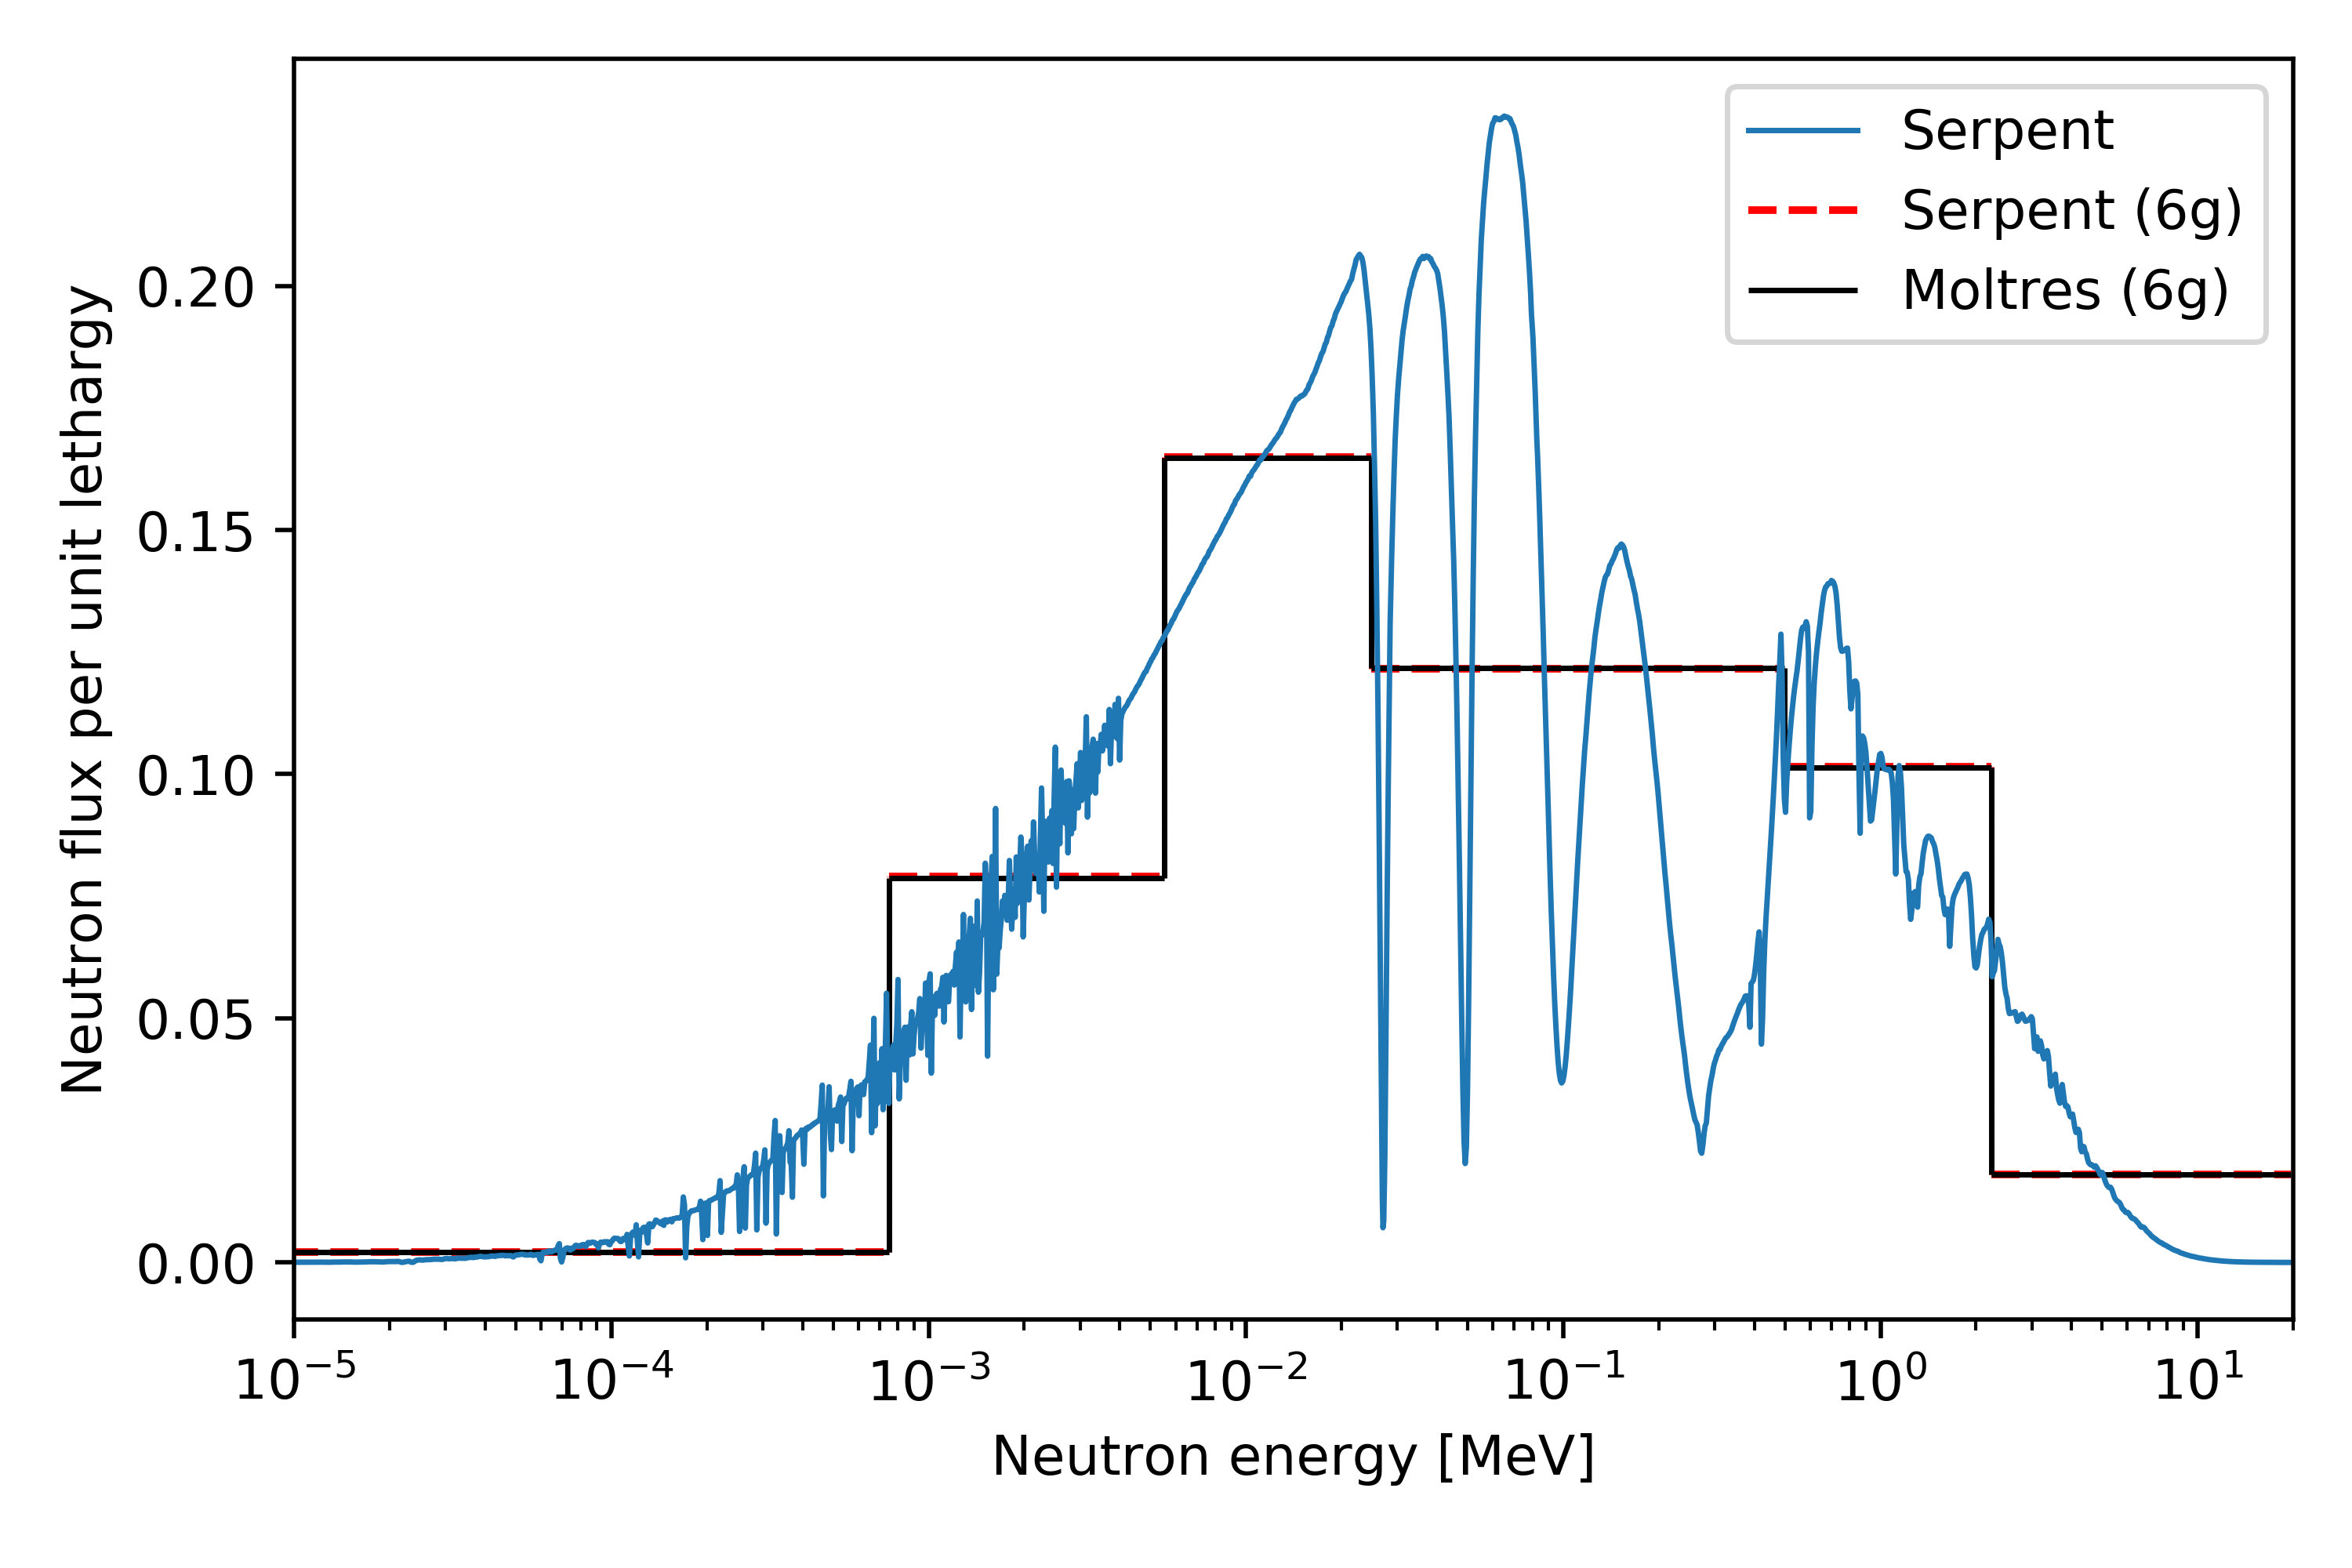
\includegraphics[width=.8\textwidth]{nt-spec}
    \caption{The fine-group and six-group neutron energy spectra from Serpent
    2 and Moltres normalized per unit lethargy.}
    \label{fig:ntspec}
\end{figure}

Moltres also closely replicated the six-group neutron spectrum from the
Serpent group constants. Figure \ref{fig:ntspec} compares the neutron energy
spectra from Serpent and Moltres in the central fuel salt region. More
generally, the
plot shows the distinctive fast spectrum observed in the \gls{MSFR} with dips
in the spectrum corresponding to elastic scattering resonances from lithium
and fluorine. From this plot, we observe that the discrepancies in
$k_{\text{eff}}$ arise mainly from discretizing neutron energy into groups
rather than the neutron diffusion model itself. We could obtain a more
accurate representation of the neutronics in the \gls{MSFR} by using more
neutron energy groups but this would adversely impact simulation times in the
subsequent multiphysics finite element analyses.

In summary, Moltres replicated the relevant neutronics parameters
accurately using the group constant data from Serpent 2. Moltres agrees with
the high fidelity simulation in Serpent 2 for the $\beta_{\text{eff}}$ and
temperature reactivity coefficients, which are important parameters for
modeling transient reactor behavior. The $k_{\text{eff}}$ values have
discrepancies on the order of 100 pcm which are relatively small compared
to other \gls{MSR} multiphysics simulation tools (e.g. the neutron diffusion
and SP3 models in OpenFOAM \cite{cervi_development_2019}).


\chapter{Coupled Neutronics/Thermal-Hydraulics Steady-State Results}
With the verification of Moltres' neutronics modeling capabilities in the
context of the \gls{MSFR}, we now move on to the multiphysics simulation
results. This chapter covers the steady-state multiphysics simulation results
from Moltres.

The procedure for obtaining the steady-state results involved several steps
due to the highly coupled \glspl{PDE}. First, we ran a preliminary transient
simulation of fluid flow in the \gls{MSFR} core, starting from zero inlet
velocity and gradually ramping it up to match the nominal flow rate (4.5 m$^3$
s$^{-1}$); otherwise Moltres had difficulty converging to the desired fully
developed flow profile. We imposed a parabolic flow profile at the inlet.
Next, we imported these fully developed flow values as initial values for
velocity in the actual transient simulation modeling the full coupled
neutronics and thermal-hydraulics. The initial values for the temperature and
neutron group flux distributions are 953 K and $1 \times 10^{14}$ cm$^{-2}$
s$^{-1}$ uniformly throughout the geometry. Finally, we assume that steady
state is reached when the volume integral values of every variable remain
constant (up to 6 sig. fig.) for at least four seconds in the simulation; this
time period corresponds to the nominal circulation time of the \gls{MSFR}.

For a direct comparison with the steady-state results from the Polimi and
TUDelft models \cite{aufiero_development_2014}, we will first present our
steady-state results without modeling decay heat. After this comparison, we
separately discuss the minor differences borne from decay heat modeling in the
last subsection.

\section{Steady-State Thermal-Hydraulics Results}

\begin{figure}[t!]
    \centering
    \begin{subfigure}[t]{.365\textwidth}
        \centering
        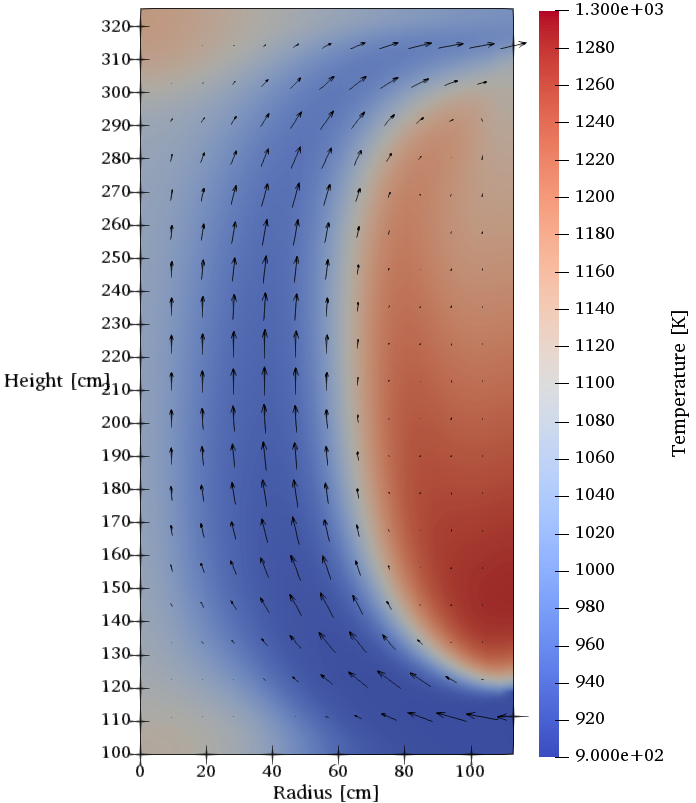
\includegraphics[width=\textwidth]{flow-temp}
    \end{subfigure}
    \hfill
    \begin{subfigure}[t]{.625\textwidth}
        \centering
        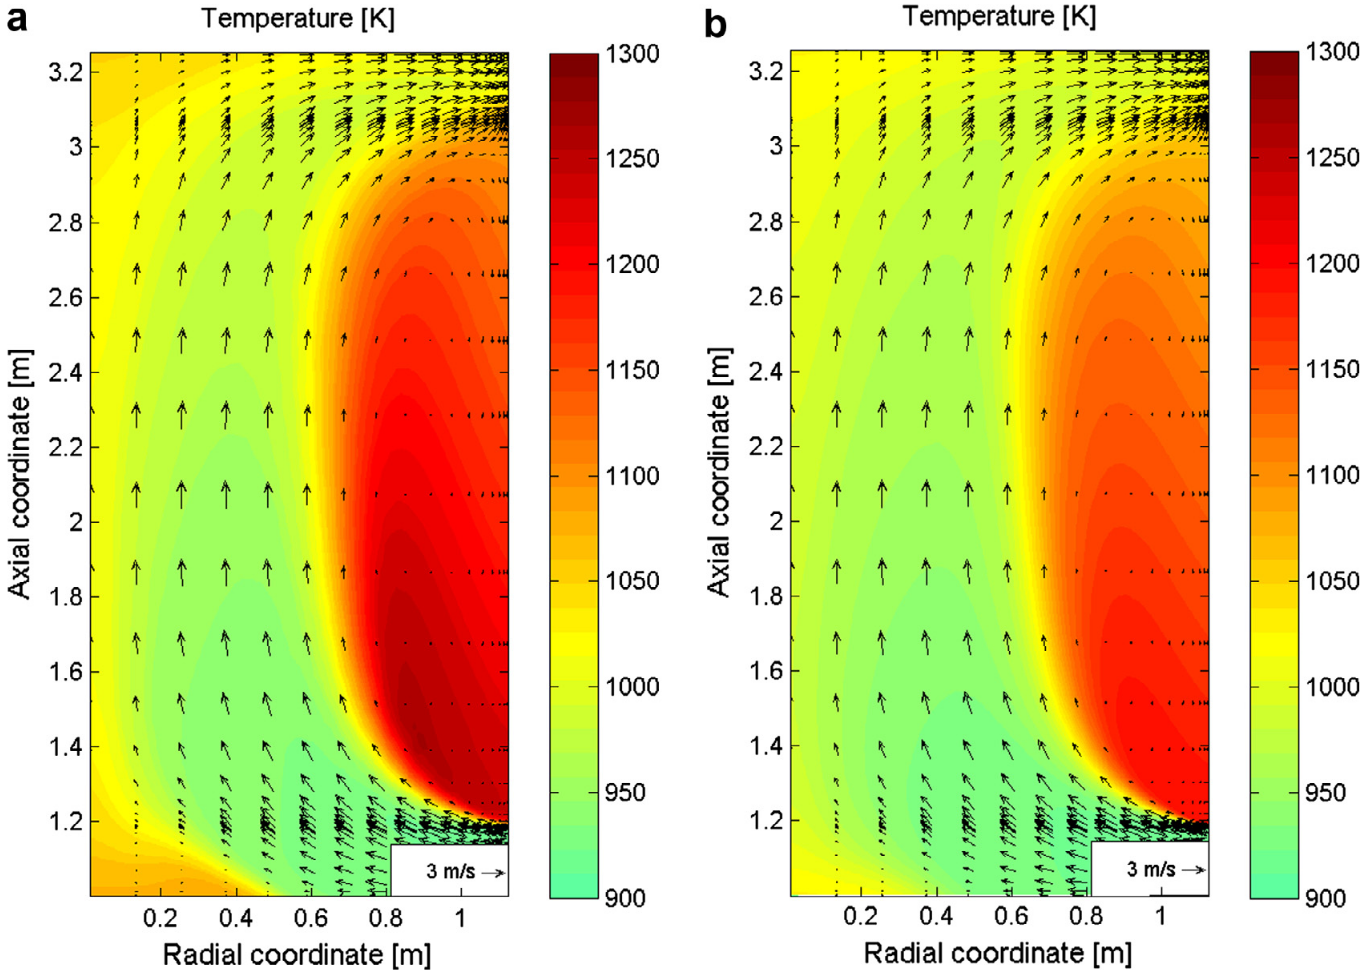
\includegraphics[width=\textwidth]{flow-temp-fiorina}
    \end{subfigure}
    \caption{Temperature and velocity fields in the core from Moltres
    (left), Polimi (center), and TUDelft (right) models. The colors represent
    temperature according to the respective colorbars and the arrows
    represent velocity fields.}
    \label{fig:flow-temp}
\end{figure}

\begin{figure}[t!]
    \centering
    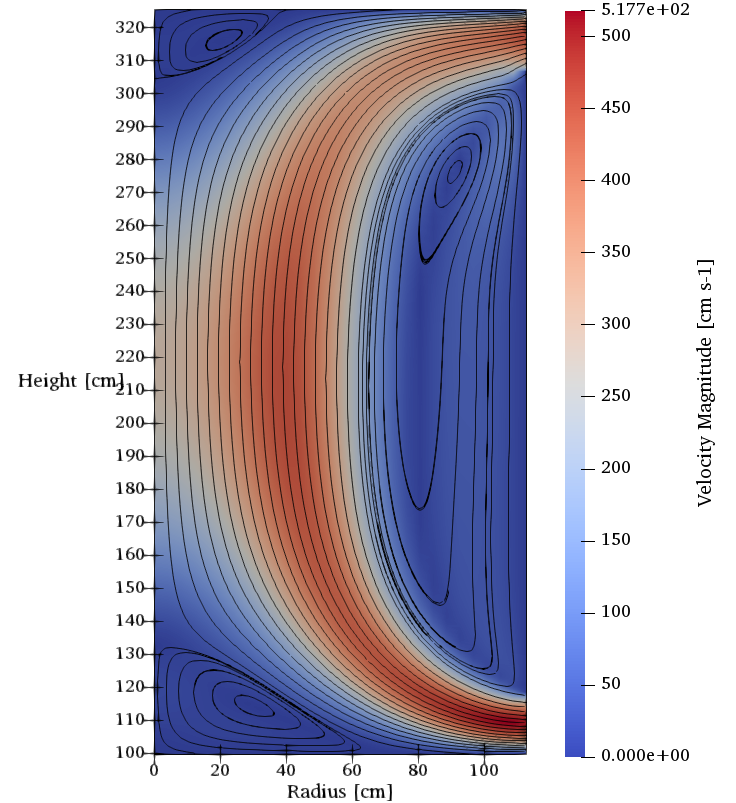
\includegraphics[width=.6\textwidth]{flow}
    \caption{Fuel salt flow streamlines and velocity magnitude in the core.
    The colors represent velocity magnitude according to the colorbar on the
    right.}
    \label{fig:flow}
\end{figure}

Figure \ref{fig:flow-temp} shows the temperature and velocity fields of the
fuel salt in the core at steady state from Moltres and the Polimi and TUDelft
models. Figure \ref{fig:flow} provides an alternate view of the flow profile
through flow streamlines superimposed on the velocity magnitude distribution.
The results from Moltres show good qualitative agreement with the
Polimi and TUDelft models \cite{fiorina_modelling_2014}; we observe similar
flow and hotspot features in all three models. Furthermore, the highest salt
velocities in all three models occur at the inlet, outlet, and at core
half-height approximately 0.40 m away from the central axis. There is a large
recirculation region near the blanket tank walls arising from turbulent flow.
Inertial forces dominate over viscous forces to form this large eddy. The main
difference between Moltres and Fiorina et al.'s models is the flow profile
near the central axis at the top and bottom of the core.
The Polimi and TUDelft models predict relatively stagnant flow in these
regions without recirculation. Moltres, on the other hand, predicts explicit
recirculating flow in these regions. This is due to our constant turbulent
viscosity approximation in Moltres. The k-$\epsilon$ turbulence models in the
Polimi and TUDelft models predict that the turbulent viscosity in these
regions is as high as 100 Pa s, much higher than our 40 Pa s approximation.

Nevertheless, similar temperature hotspots form in these regions of
recirculation and stagnation as convection is the dominant heat transfer
mechanism. The maximum temperature from Moltres, 1275 K near the bottom of the
large recirculation zone, is closer to the maximum temperature in the Polimi
model ($\approx$ 1300 K) than the TUDelft model ($\approx$ 1200K). Similarly,
we observe cooler temperatures in high-velocity regions. The minimum
temperature is 924 K at the inlet. 

Although the temperatures at the hotspots are well below the melting point of the Ni-alloy structure (1500 K), they may cause undue thermal stress on the
blanket tank structure and induce relatively faster salt corrosion rates. A
sudden, large reactivity insertion could push fuel salt temperatures above the
melting point of the Ni-alloy and cause irreversible damage. Furthermore,
the reservoir of hot fuel salt may cause unpredictable behavior during
transient scenarios when the flow profile undergoes a drastic change.
Thus, Rouch et al. \cite{rouch_preliminary_2014} developed an improved
hourglass-shaped design to optimize flow distribution and prevent these
recirculation zones and hotspots from forming. A study of this new design
using Moltres is a potential subject for future work when a proper turbulence
model is in place.

\section{Steady-State Neutronics Results}

\subsection{Neutron Flux}

The neutron flux distribution represents the heat source distribution in a
nuclear reactor. Figure \ref{fig:neutronflux} shows the neutron flux
distributions in the core for all six neutron energy groups, and Figure
\ref{fig:axialradial} shows the axial and radial fluxes along the center of
the core and at reactor half-height, respectively.
The distributions are highly symmetric along the
central and horizontal axes, as expected of a cylindrical reactor design. The
relatively lower temperatures near the center of the core promotes the neutron
flux peaking but it is not a major concern as there are no structural parts
vulnerable to neutron damage in that region. The peak total flux at the center
is $9.80 \times 10^{15}$ cm$^{-2}$ s$^{-1}$, which is close to values reported
by Fiorina et al. \cite{fiorina_molten_2013} and Aufiero et al.
\cite{aufiero_development_2014} as shown in Table \ref{table:peak-flux}. The
peak flux value from this paper is slightly higher as we used the steady-state
temperature distribution while Fiorina et al. and Aufiero et al. imposed a
uniform temperature distribution at 973 K.

\begin{figure}[b!]
    \centering
    \begin{subfigure}[t]{.325\textwidth}
        \centering
        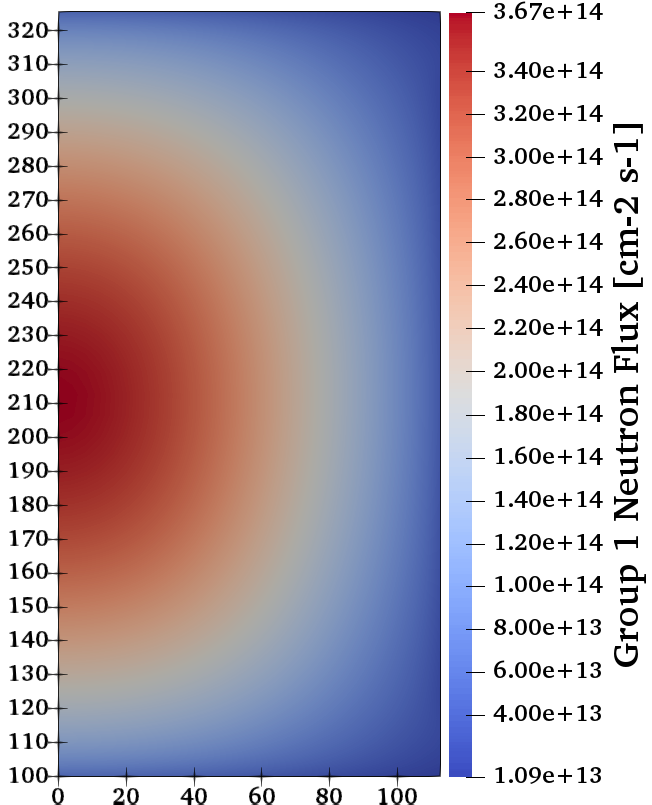
\includegraphics[width=\textwidth]{ss-g1}
    \end{subfigure}
    \begin{subfigure}[t]{.325\textwidth}
        \centering
        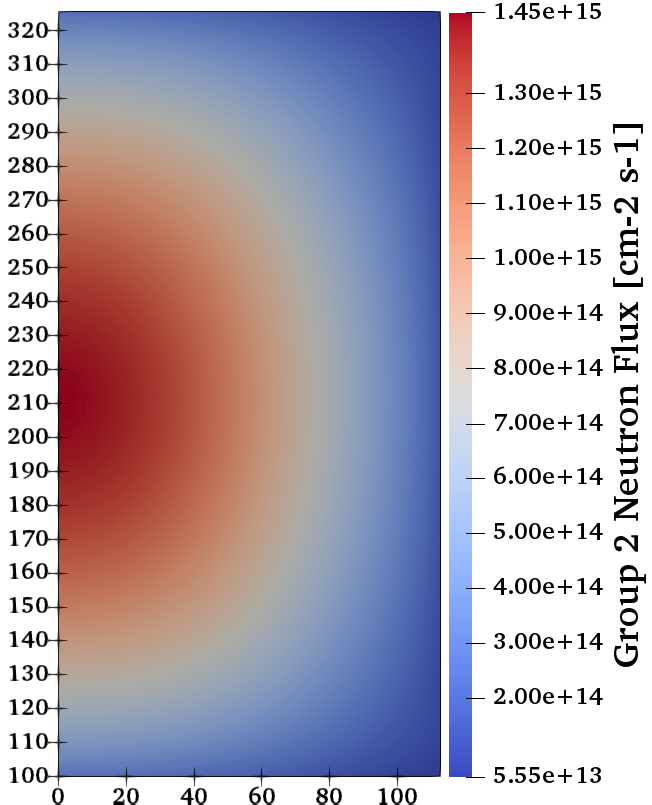
\includegraphics[width=\textwidth]{ss-g2}
    \end{subfigure}
    \begin{subfigure}[t]{.325\textwidth}
        \centering
        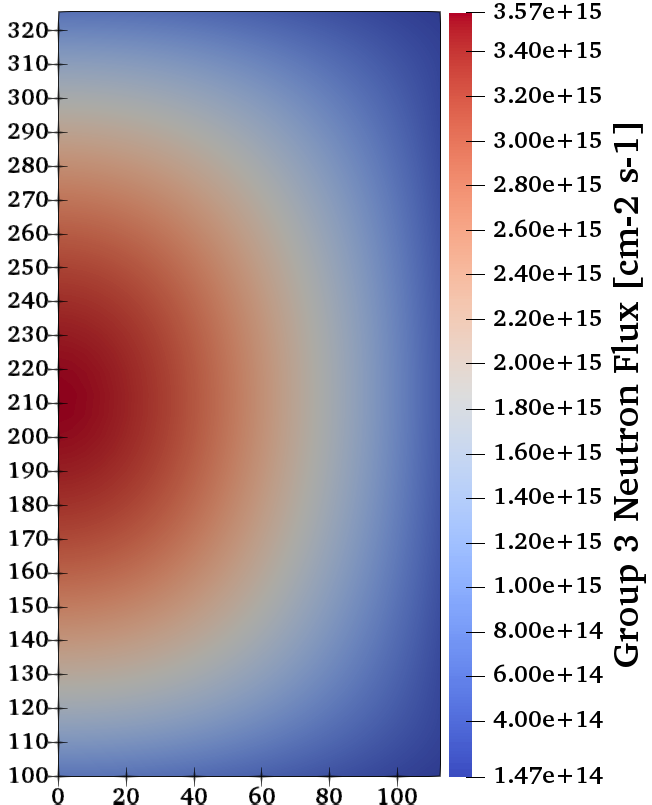
\includegraphics[width=\textwidth]{ss-g3}
    \end{subfigure}
    \begin{subfigure}[t]{.325\textwidth}
        \centering
        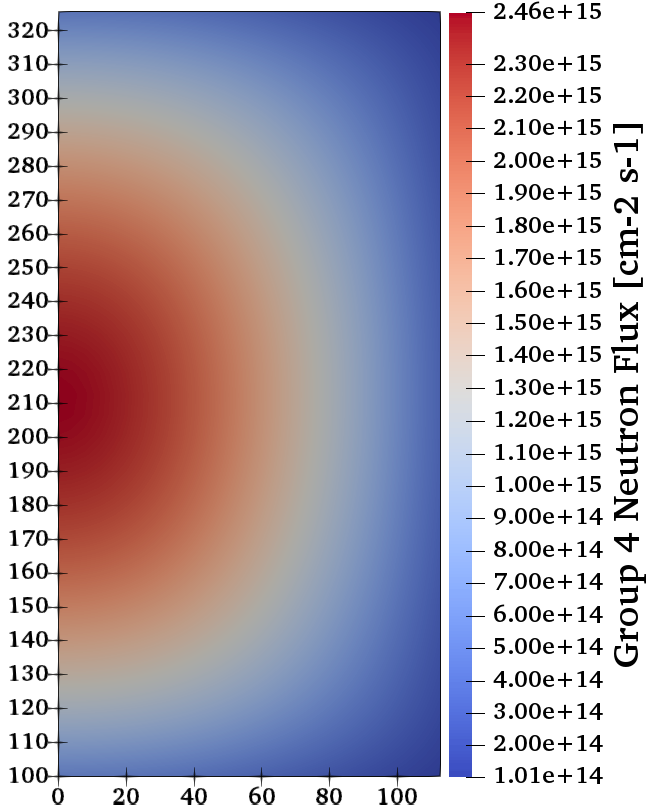
\includegraphics[width=\textwidth]{ss-g4}
    \end{subfigure}
    \begin{subfigure}[t]{.325\textwidth}
        \centering
        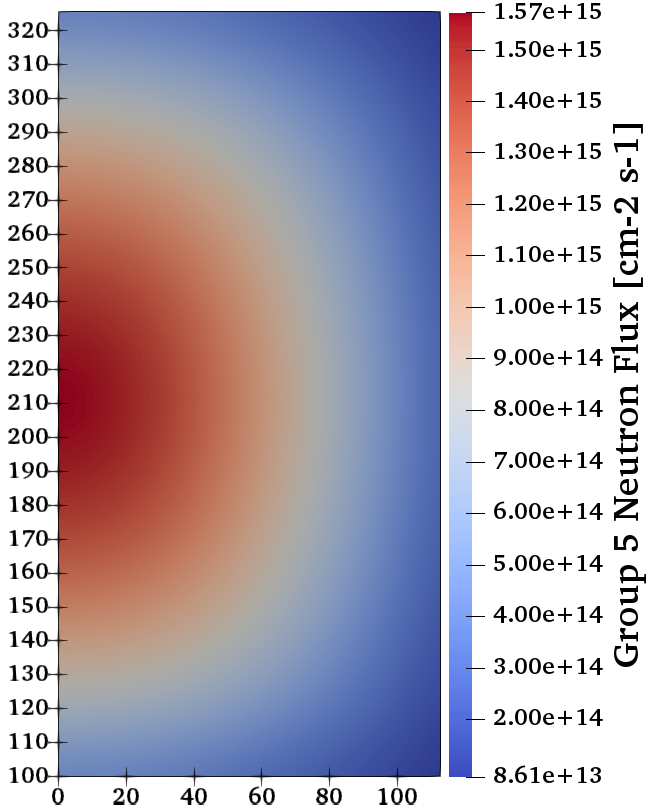
\includegraphics[width=\textwidth]{ss-g5}
    \end{subfigure}
    \begin{subfigure}[t]{.325\textwidth}
        \centering
        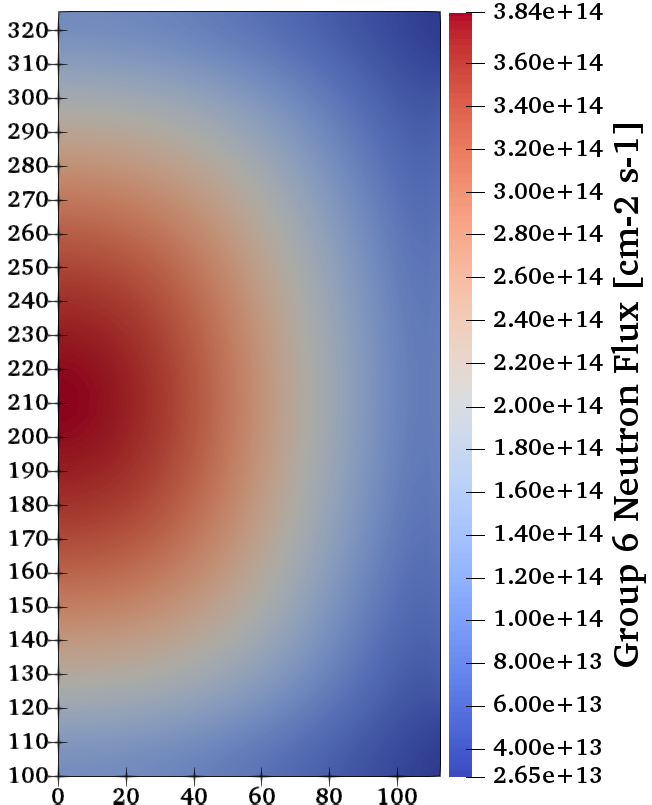
\includegraphics[width=\textwidth]{ss-g6}
    \end{subfigure}
    \caption{Neutron flux distributions in the core for neutron energy groups
    1 to 6. The y and x axes represent height and radius (in cm) of the core
    relative to the entire reactor geometry.}
    \label{fig:neutronflux}
\end{figure}

\begin{figure}[t!]
    \centering
    \begin{subfigure}[t]{.49\textwidth}
        \centering
        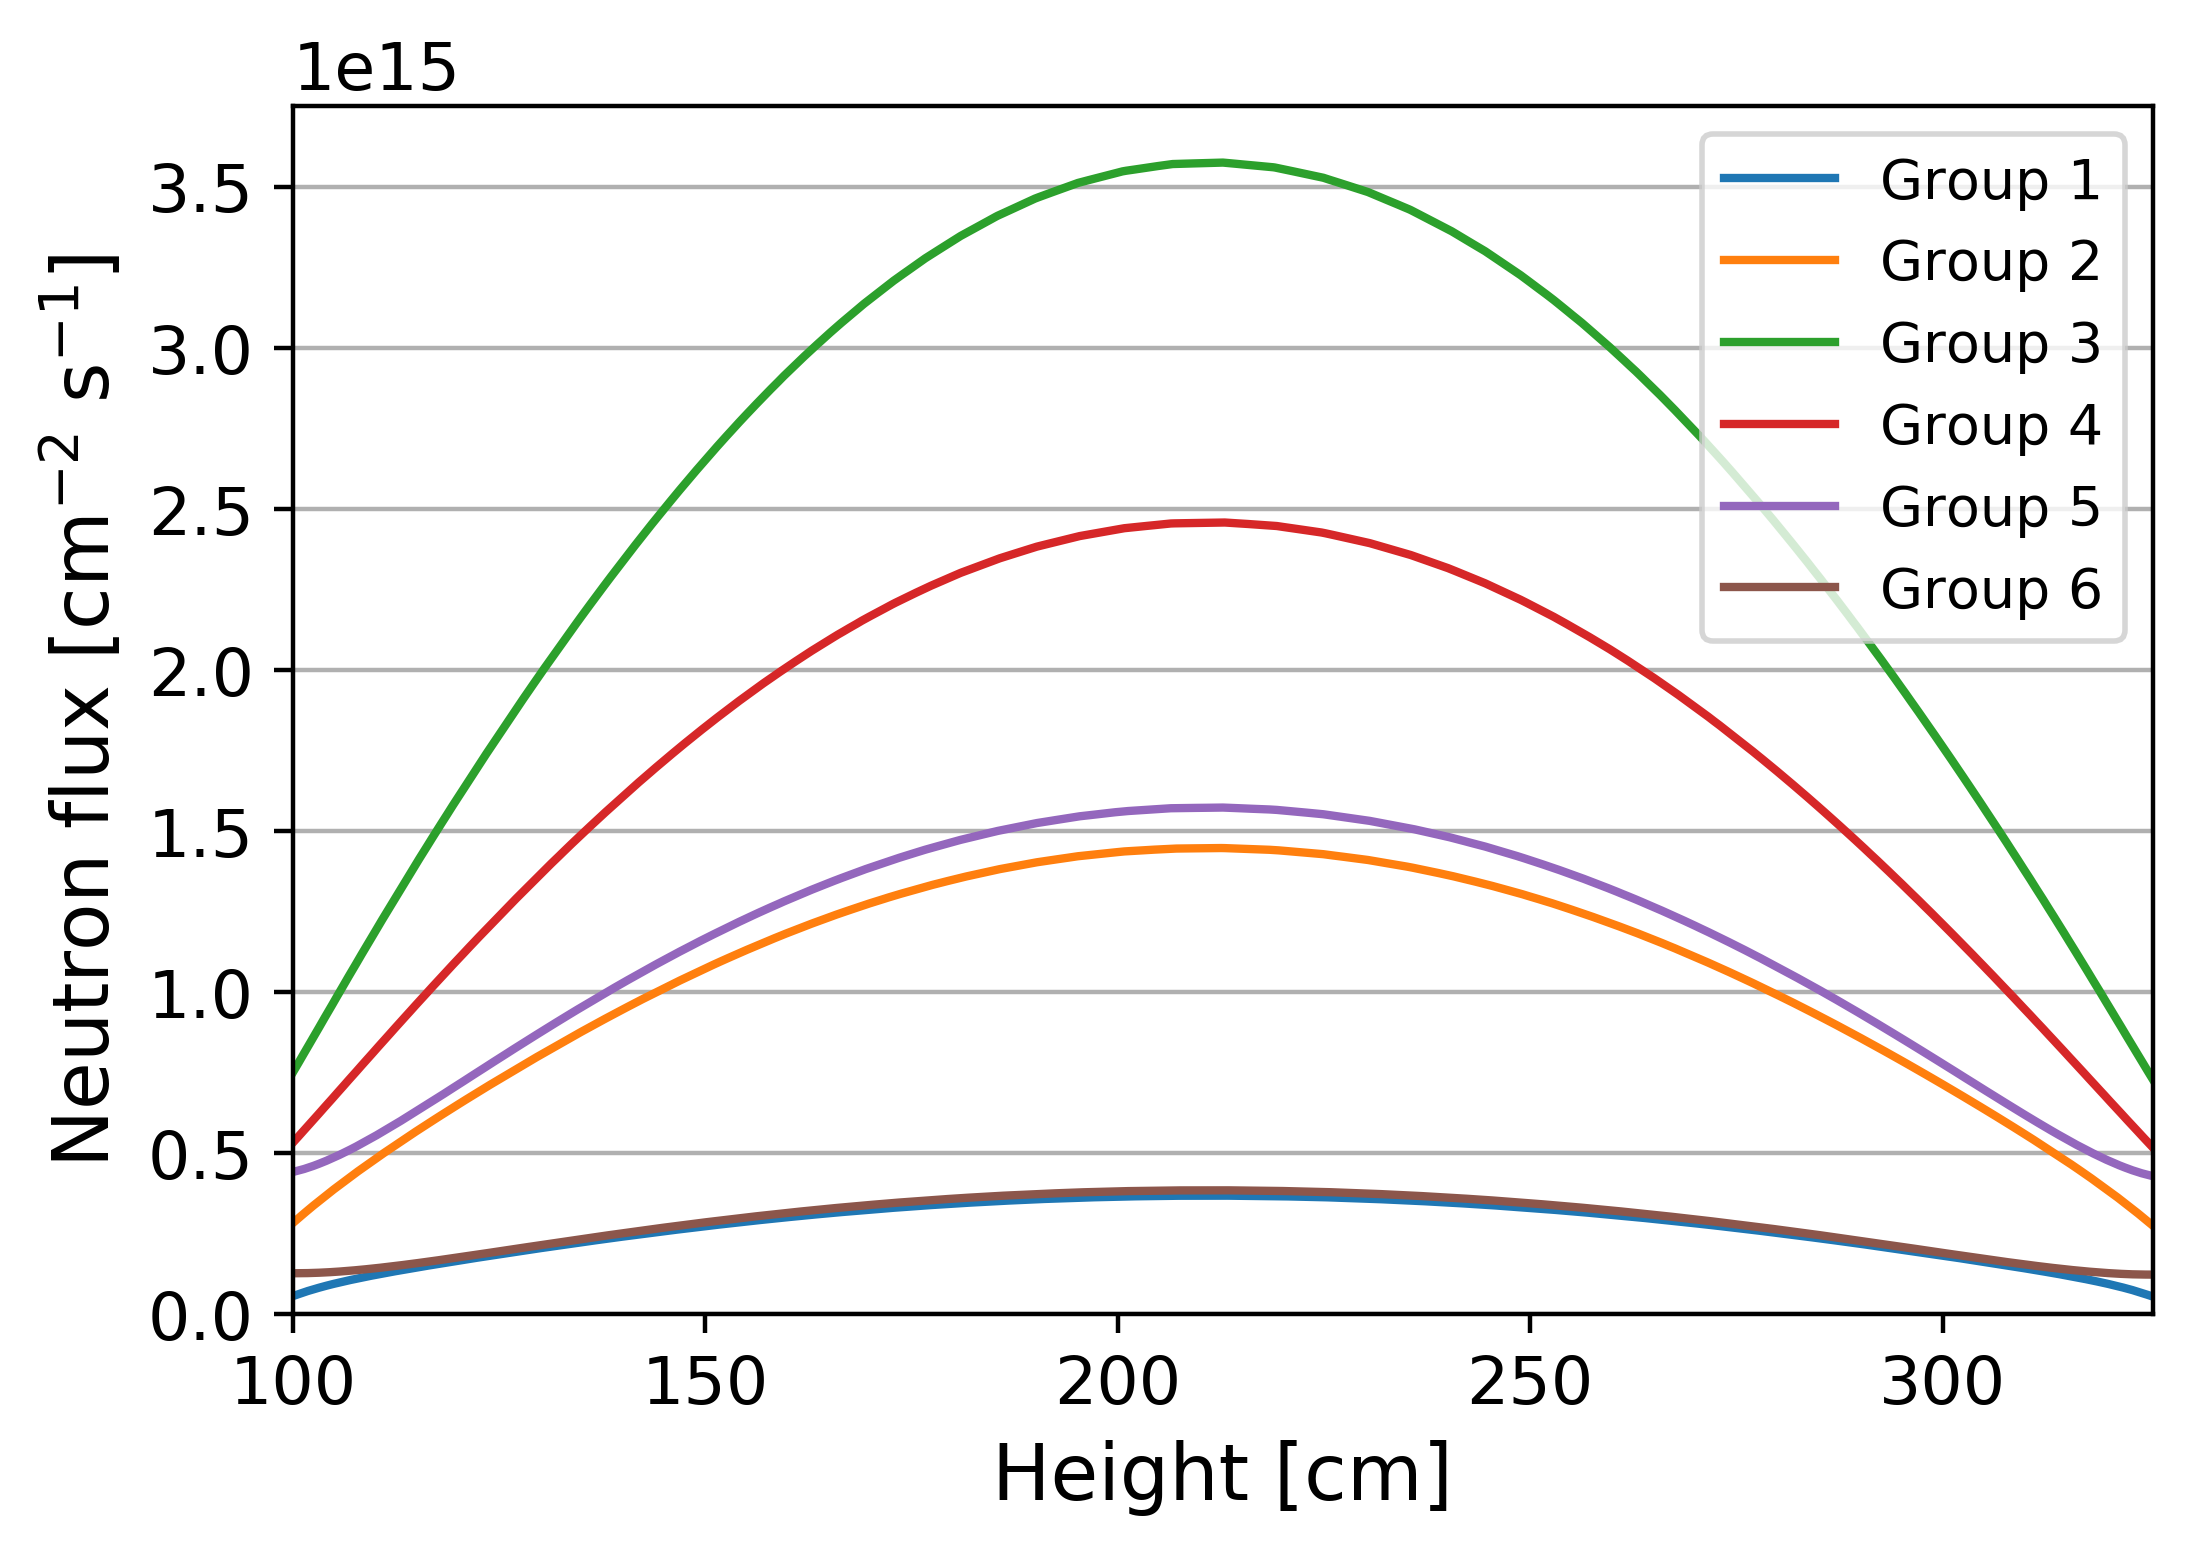
\includegraphics[width=\textwidth]{axial-flux}
    \end{subfigure}
    \begin{subfigure}[t]{.49\textwidth}
        \centering
        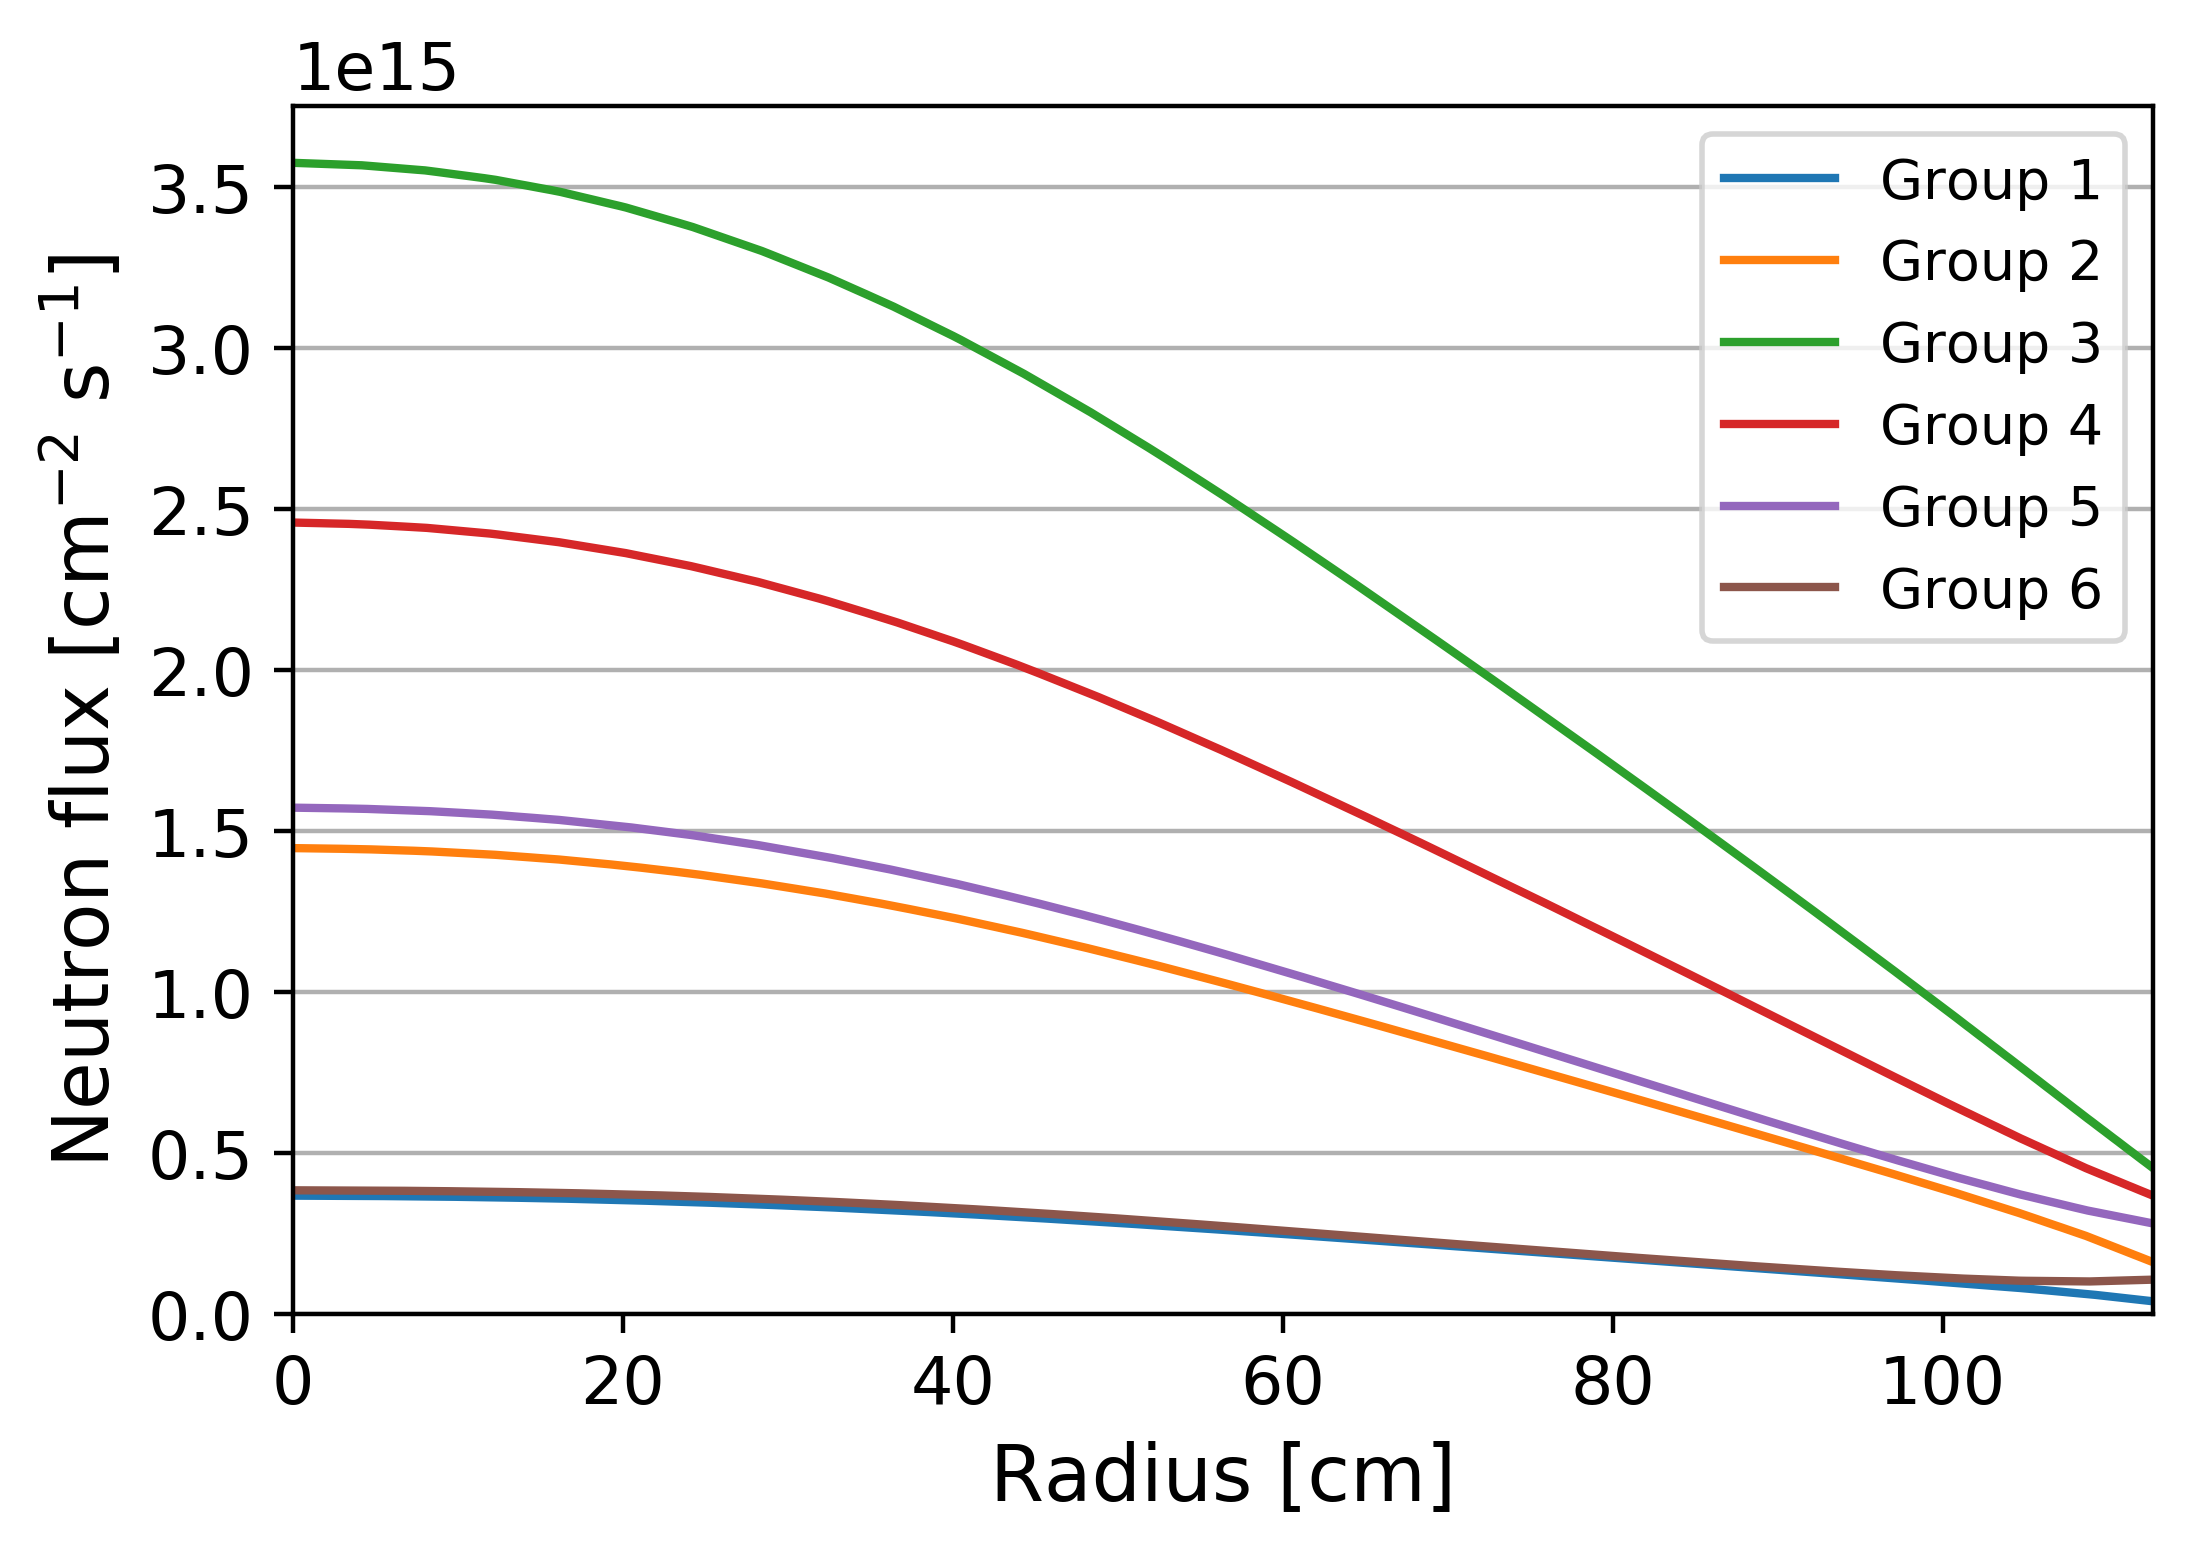
\includegraphics[width=\textwidth]{radial-flux}
    \end{subfigure}
    \caption{Axial (left) and radial (right) neutron flux distributions in the
    core for neutron energy groups 1 to 6.}
    \label{fig:axialradial}
\end{figure}

\begin{table}[b!]
	\centering
	\caption{Peak neutron flux values from Moltres (this paper), COMSOL
	\cite{fiorina_molten_2013}, and OpenFOAM \cite{aufiero_development_2014}
	models along with the temperature distribution with which the values were
	obtained.}
	\begin{tabular}{l l S}
		\toprule
		{Model} & {Temperature distribution} & {Peak Neutron Flux [$\times 10^{15}$ cm$^{-2}$ s$^{-1}$]}
		\\
		\midrule
		{Moltres (This paper)} & {Steady state} & 9.80\\
		{COMSOL} & {Uniform, 973 K} & 8.6 \\
		{OpenFOAM} & {Uniform, 973 K} & 9.0 \\
		\bottomrule
	\end{tabular}
	\label{table:peak-flux}
\end{table}

\begin{figure}[t!]
    \centering
    \begin{subfigure}[t]{.243\textwidth}
        \centering
        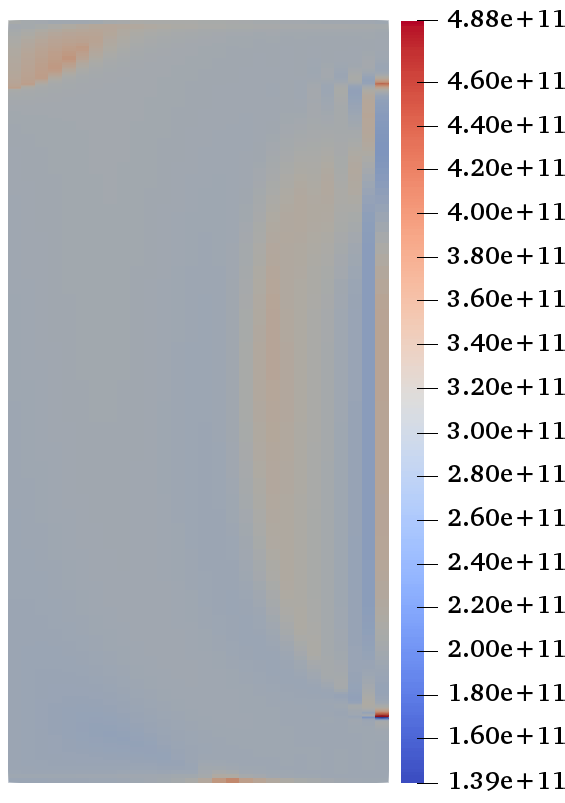
\includegraphics[width=\textwidth]{ss-pre1}
    \end{subfigure}
    \begin{subfigure}[t]{.243\textwidth}
        \centering
        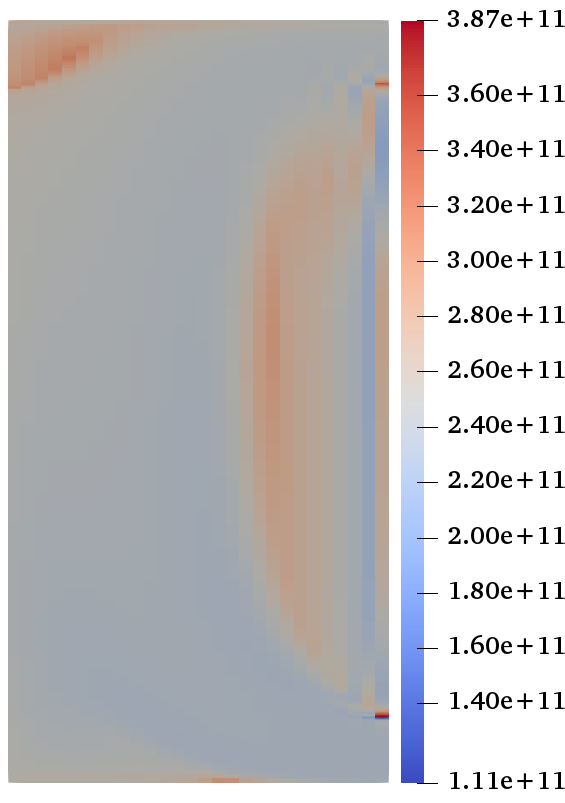
\includegraphics[width=\textwidth]{ss-pre2}
    \end{subfigure}
    \begin{subfigure}[t]{.243\textwidth}
        \centering
        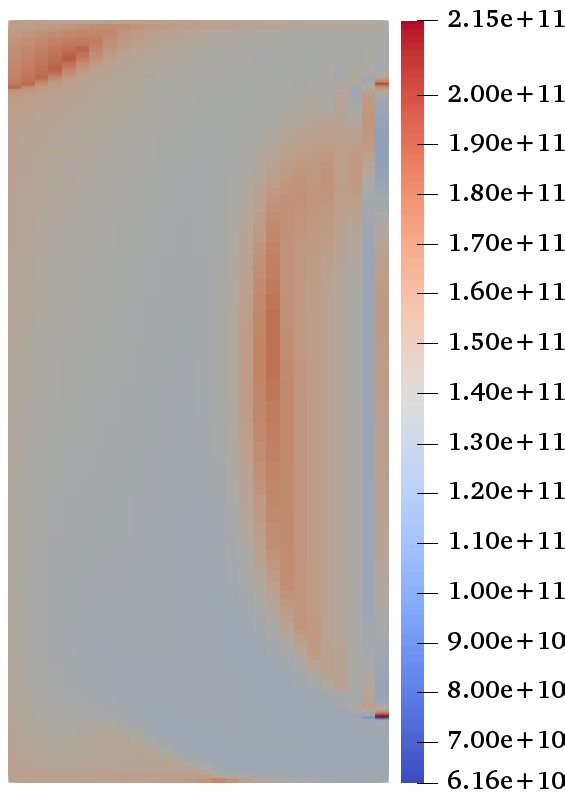
\includegraphics[width=\textwidth]{ss-pre3}
    \end{subfigure}
    \begin{subfigure}[t]{.243\textwidth}
        \centering
        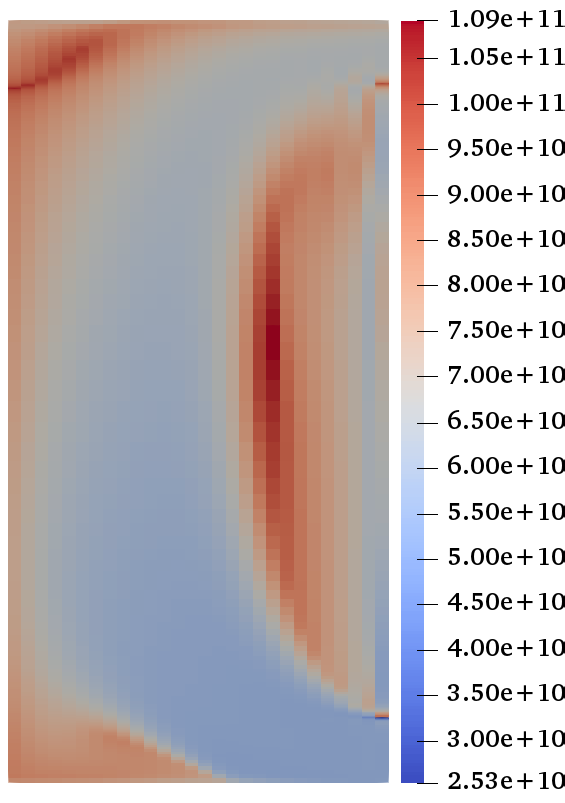
\includegraphics[width=\textwidth]{ss-pre4}
    \end{subfigure}
    \begin{subfigure}[t]{.243\textwidth}
        \centering
        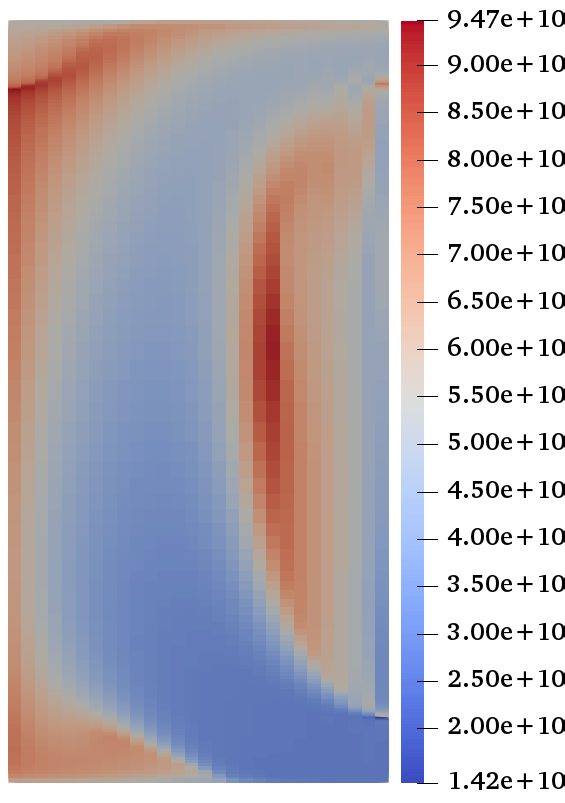
\includegraphics[width=\textwidth]{ss-pre5}
    \end{subfigure}
    \begin{subfigure}[t]{.243\textwidth}
        \centering
        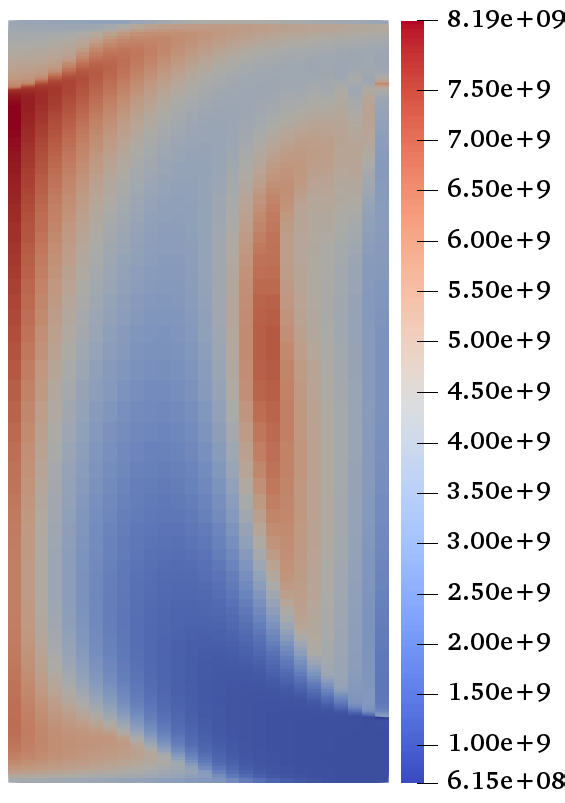
\includegraphics[width=\textwidth]{ss-pre6}
    \end{subfigure}
    \begin{subfigure}[t]{.243\textwidth}
        \centering
        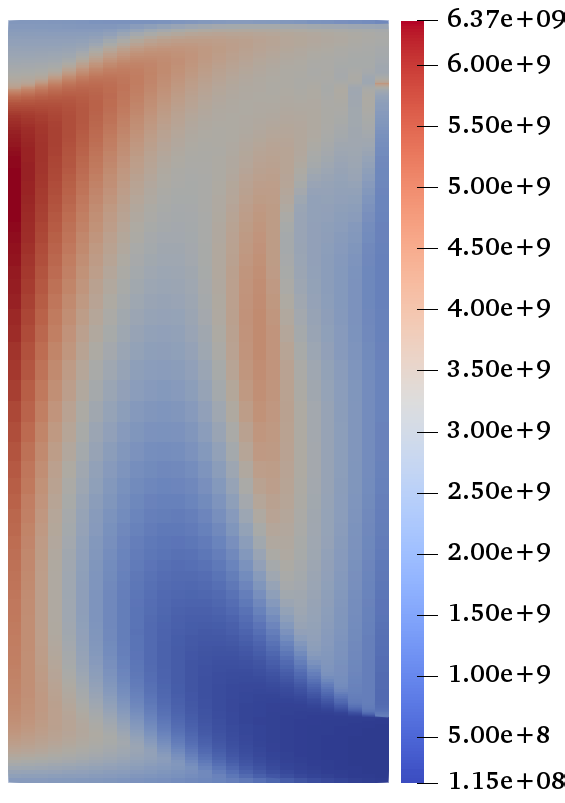
\includegraphics[width=\textwidth]{ss-pre7}
    \end{subfigure}
    \begin{subfigure}[t]{.243\textwidth}
        \centering
        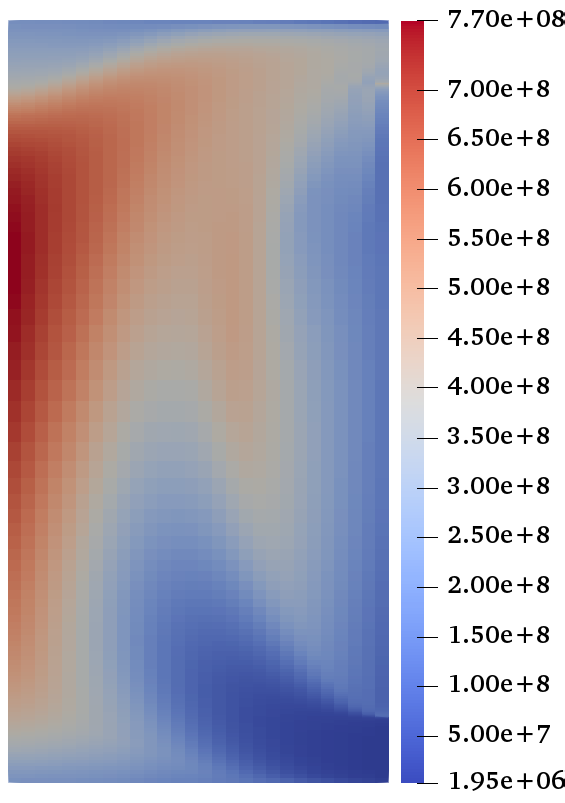
\includegraphics[width=\textwidth]{ss-pre8}
    \end{subfigure}
    \caption{\gls{DNP} distributions in the core for \gls{DNP} groups
    1 to 8 (from left to right, top to bottom). Refer to Figure \ref{fig:neutronflux} for the height and radius
    scales on the y and x axes, respectively. Note the different scales for
    each distribution.}
    \label{fig:dnp}
\end{figure}

\subsection{Delayed Neutron Fraction}

As mentioned earlier, the delayed neutron precursors (DNPs) are mobile in
\glspl{MSR} and their distributions do not directly correspond to the neutron
flux distributions. The location where the \glspl{DNP} decay and emit neutrons
impacts their neutron
importance depending on their proximity to fissile and parasitic isotopes.
Figure \ref{fig:dnp} shows the \gls{DNP} distributions for all eight \gls{DNP}
groups. In general, we observe less \glspl{DNP} in the regions with fast salt
flow, namely
 The
precursors from the shortest-lived group (Group 8) predominantly decay within
the core as their half-lives are shorter than the time it takes to reach the
outlet while the precursors from the longest-lived group (Group 1) are
relatively evenly distributed due to their long half-lives. For the
longer-lived groups, the \gls{DNP} concentrations are not well-resolved on the
mesh elements adjacent to the outlet and the inlet boundaries, respectively.
Thus, we recommend careful mesh refinement for future work involving similar
geometries.

\begin{figure}[b!]
    \centering
    \begin{subfigure}[t]{.30\textwidth}
        \centering
        \vspace{.9cm}
        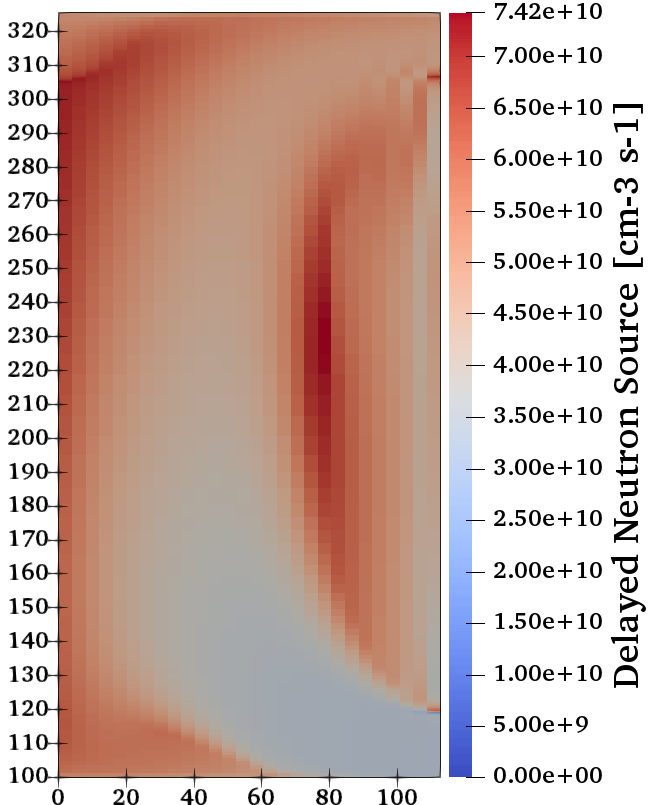
\includegraphics[width=\textwidth]{ss-pre}
    \end{subfigure}
    \begin{subfigure}[t]{.69\textwidth}
        \centering
        \vspace{0pt}
        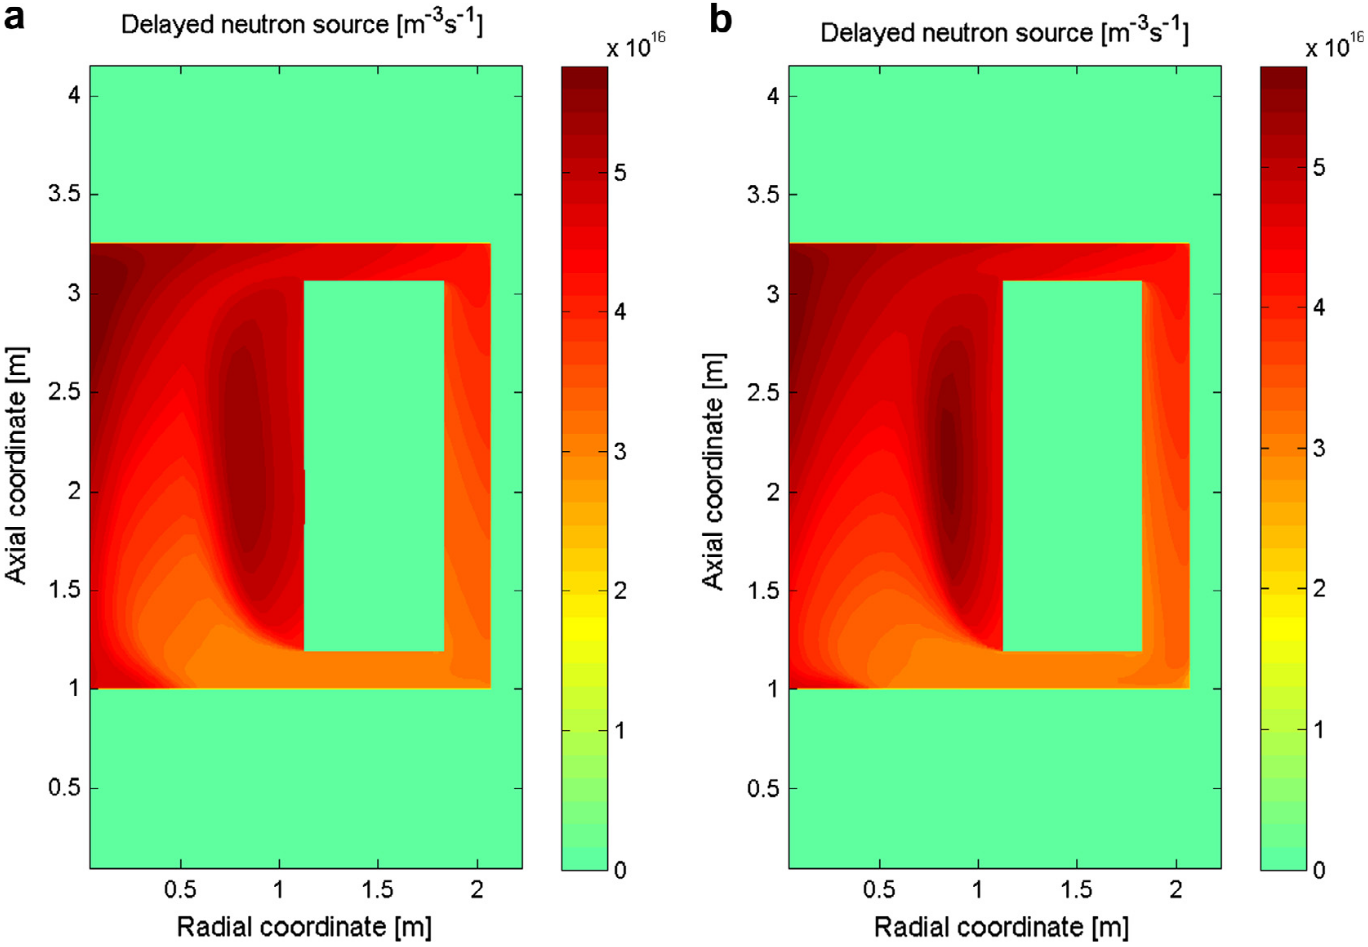
\includegraphics[width=\textwidth]{fiorina-pre}
    \end{subfigure}
    \caption{Total delayed neutron source distribution in the core from
    Moltres (left), Polimi (center), and TUDelft (right) models.}
    \label{fig:pre}
\end{figure}

In Figure \ref{fig:pre}, we compare the total delayed neutron source
distribution from Moltres with the results from the Polimi and TUDelft models
\cite{fiorina_modelling_2014}. In contrast to Figure \ref{fig:dnp} which shows
the precursor distribution, Figure \ref{fig:pre} shows the rate of delayed
neutron emission, which we calculated by multiplying each \gls{DNP} group
$C_i$ with its associated decay constant $\lambda_i$.
We observe that the Polimi and TUDelft models
feature greater \gls{DNP} retention in the stagnant regions within the core.
This effect is less pronounced in the Moltres model. There is less build-up
of \glspl{DNP} at the top of the core in Moltres because most of the
\glspl{DNP} produced near the center of the core cannot enter the axial
recirculation zone that only appears in Moltres. We also observe less build-up
in the large recirculation zone near the blanket tank.

The in-core delayed neutron fraction $\beta_c$ is an important safety
parameter for \glspl{MSR}. This value represents the actual delayed
neutron fraction in \glspl{MSR} after accounting for the loss of delayed
neutrons from \glspl{DNP} decaying outside the active core region. In general,
reactors with smaller $\beta$ values exhibit greater prompt jumps in the
neutron flux in response to reactivity insertions because they have a greater
proportion of prompt neutrons under normal operating conditions. This is
undesirable from a reactor safety perspective because it exposes the reactor
to relatively more extreme conditions before active safety mechanisms
activate and scram the reactor. In \glspl{MSR}, this danger is partly
mitigated by the strong, negative fuel temperature reactivity coefficient. 
Chapter 6 contains more in-depth discussions for various transient scenarios.

In Table \ref{table:dnf}, we compare the fraction of out-of-core emissions and
the $\beta_c$ values from Moltres with the Polimi and TUDelft models. We
calculated the fraction of out-of-core emissions by finding the total amount
of each \gls{DNP} group in the core and the outer loop, multiplying each total
by their associated decay time constants $\lambda_i$, and calculating the
proportion of emissions in the outer loop relative to the grand total. We
calculated $\beta_c$ by first obtaining the prompt neutron emission rate from
Moltres and subsequently using in-core delayed neutron emission rate from the
previous calculation to find the fraction of delayed neutron emission rate
relative to total emission rate.

\begin{table}[t!]
	\centering
	\caption{The fraction of delayed neutrons lost from out-of-core emission
	and the in-core delayed neutron fraction $\beta_c$ values from Moltres
	(this paper), and the Polimi and TUDelft models
	\cite{fiorina_modelling_2014}.}
	\begin{tabular}{l S S}
		\toprule
		{Model} & {Out-of-Core Emission [\%]} & {$\beta_c$ [pcm]}
		\\
		\midrule
		{Moltres (This paper)} & {44.16} & {184.9}\\
		{Polimi} & {34.80} & {134.3} \\
		{TUDelft} & {34.85} & {123.8} \\
		\bottomrule
	\end{tabular}
	\label{table:dnf}
\end{table}

The fraction of out-of-core emissions from our Moltres model
differs significantly by approximately 10\%, and $\beta_c$ differs by
60-70 pcm. We attribute the former to the lesser \gls{DNP} retention in the
stagnant flow regions in the core; the \glspl{DNP} are more evenly distributed
along the entire primary loop, leading to more delayed neutron emissions in
the outer loop region. The most likely reason for this is differences in the
flow pattern in the recirculation zone because convective species transport
dominates diffusive effects in the \gls{MSFR}. The exact flow pattern in the
recirculation zones in the Polimi and TUDelft models is likely to differ from
that in Moltres (Figure \ref{fig:flow}). Figure \ref{fig:flow-temp} also shows
some minor differences in the magnitude of the flow in the recirculation zones
between Moltres, and the Polimi and TUDelft models. Although the sizes of the
arrows representing flow velocity are not normalized to the same scales, a
quick comparison between the largest arrows and the arrows in the
recirculation zone indicate that the recirculation zone in Moltres is
relatively more stagnant. This could explain the concentration of \glspl{DNP}
along an ``arc'' closer to the center of the core in Moltres as opposed to the
more even distribution of \glspl{DNP} throughout the whole recirculation zones
in the Polimi and TUDelft models. The higher peak \glspl{DNP} distribution in
Moltres also supports this assertion.

In spite of the greater delayed neutron losses, the $\beta_c$ value is higher
in Moltres than the Polimi and TUDelft models. To account for this
peculiarity, we note that Fiorina et al. \cite{fiorina_modelling_2014}
applied adjoint flux weighting for their $\beta_c$ calculation whereas we
report our value as the physical fraction without adjoint weighting. The
weighting results in a significant difference in $\beta_c$ because a large
fraction of the \glspl{DNP} decay in the recirculation zones, where the
neutron importance is noticeably diminished.

\section{Decay Heat}

The inclusion of a decay heat model effectively redistributes a fraction of
the volumetric heat source from the center of the core to the entire loop.
Thus, we expect to observe a slight flattening of the temperature distribution
across the entire primary loop.


\chapter{Transient Scenarios}
This chapter discusses the transient multiphysics simulation results of the
\gls{MSFR} from Moltres for four accident scenarios. These scenarios, adapted
from Fiorina et al.'s work \cite{fiorina_modelling_2014}, include unprotected
instances of reactivity insertion, loss of heat sink, loss of flow, and pump
overspeed accidents. The term ``unprotected'' means no external interventions
occur in these scenarios. As such, these simulations
give an insight on the \gls{MSFR}'s passive safety capabilities in the absence
of any active safety system. This work used the steady-state configuration
presented in the previous chapter as the initial conditions for the transient
simulations discussed in this chapter. Specifically, all steady-state spatial
values for neutron flux, delayed neutron precursor concentration, temperature,
velocity, and pressure were imported as the initial state of the transient
scenarios.

As noted by Fiorina et al. \cite{fiorina_modelling_2014}, explicit decay heat
modeling has a negligible effect in reactivity-, and pump-initiated
transients. Furthermore, only their Polimi model had decay
heat modeling capabilities. Therefore, they presented results from their
Polimi and TUDelft model for the four accident scenarios without decay heat
modeling and enabled decay heat modeling for the loss of heat sink transient
scenario only. This work also ran all transient simulations without the decay
heat model for a fair comparison. The only exception is loss of heat sink
scenario in which two separate simulations with and without the decay heat
model were run. More generally, this work imposed various other simplifying
assumptions in our transient models to match their implementations as closely
as possible, within Moltres' capabilities. The details of the setup for each
transient simulation are in their respective sections.

\section{Unprotected Reactivity Insertion}

Reactivity insertion accidents are a type of nuclear accident caused by
unintended positive
reactivity insertions. The excess reactivity causes the power output and
temperatures in nuclear reactors to rise to potentially dangerous levels. In
\glspl{MSR}, a positive reactivity insertion could occur when the online
refueling system injects excess fissile material into the core. Excessively
high neutron fluences and temperatures negatively impact reactor structural
integrity and increase the risk of containment breach.

This work modeled two unprotected step-wise reactivity insertion scenarios in
Moltres by swapping out the original set of group constant data with two new,
separate sets of data from Serpent corresponding to 50 pcm and 200 pcm
reactivity insertions, respectively. The reactivity of the Serpent \gls{MSFR}
models was increased by increasing the $^{233}$U-to-$^{232}$Th ratio in
the fuel salt.

The focus of this transient study is the neutronic and thermal-hydraulic
behavior of the reactor core. Thus, this work assumes that the heat exchanger
and the associated power generation equipment (generator turbines, heat sinks,
etc.) can withstand all variations in the power output during the transients.

Figures \ref{fig:50pcmheat} and \ref{fig:50pcmtemp} show the power output and
average core temperature increase following the 50 pcm step-wise reactivity
insertion in the Moltres, Polimi, and TUDelft models. The initial prompt
response to the reactivity insertion raises power to 4 GW by $t=0.001$ s.
Figure \ref{fig:50pcmjump} shows the rise in power output specifically during
the prompt response in a separate plot.
Power continues to rise at a slower rate up to 4.63 GW at around $t=0.005$ s,
at which point the negative reactivity from the Doppler effect and salt
expansion becomes greater
than the initial +50 pcm insertion. Power continues to fall as the average
core temperature rises. The slight change in slope occurs at $t=0.3$ s. The
elapsed time approximately corresponds to the average half-life of the two
shortest-lived delayed neutron precursor (DNP) groups ($t_{1/2}=0.195$ s and
$0.424$ s); the decay of the surplus precursors produced in the initial phase
negates a fraction of the negative reactivity from the elevated core
temperature. By $t=3$-$4$ s, most of the heated salt and \glspl{DNP} from the
initial phase will have circulated around the primary loop and returned to the
core. The heated salt causes a small, noticeable dip in power before the power
output stabilises. The core tends to a new equilibrium average temperature
approximately 7.5 K higher than the initial average temperature.

\begin{figure}[htbp!]
    \centering
    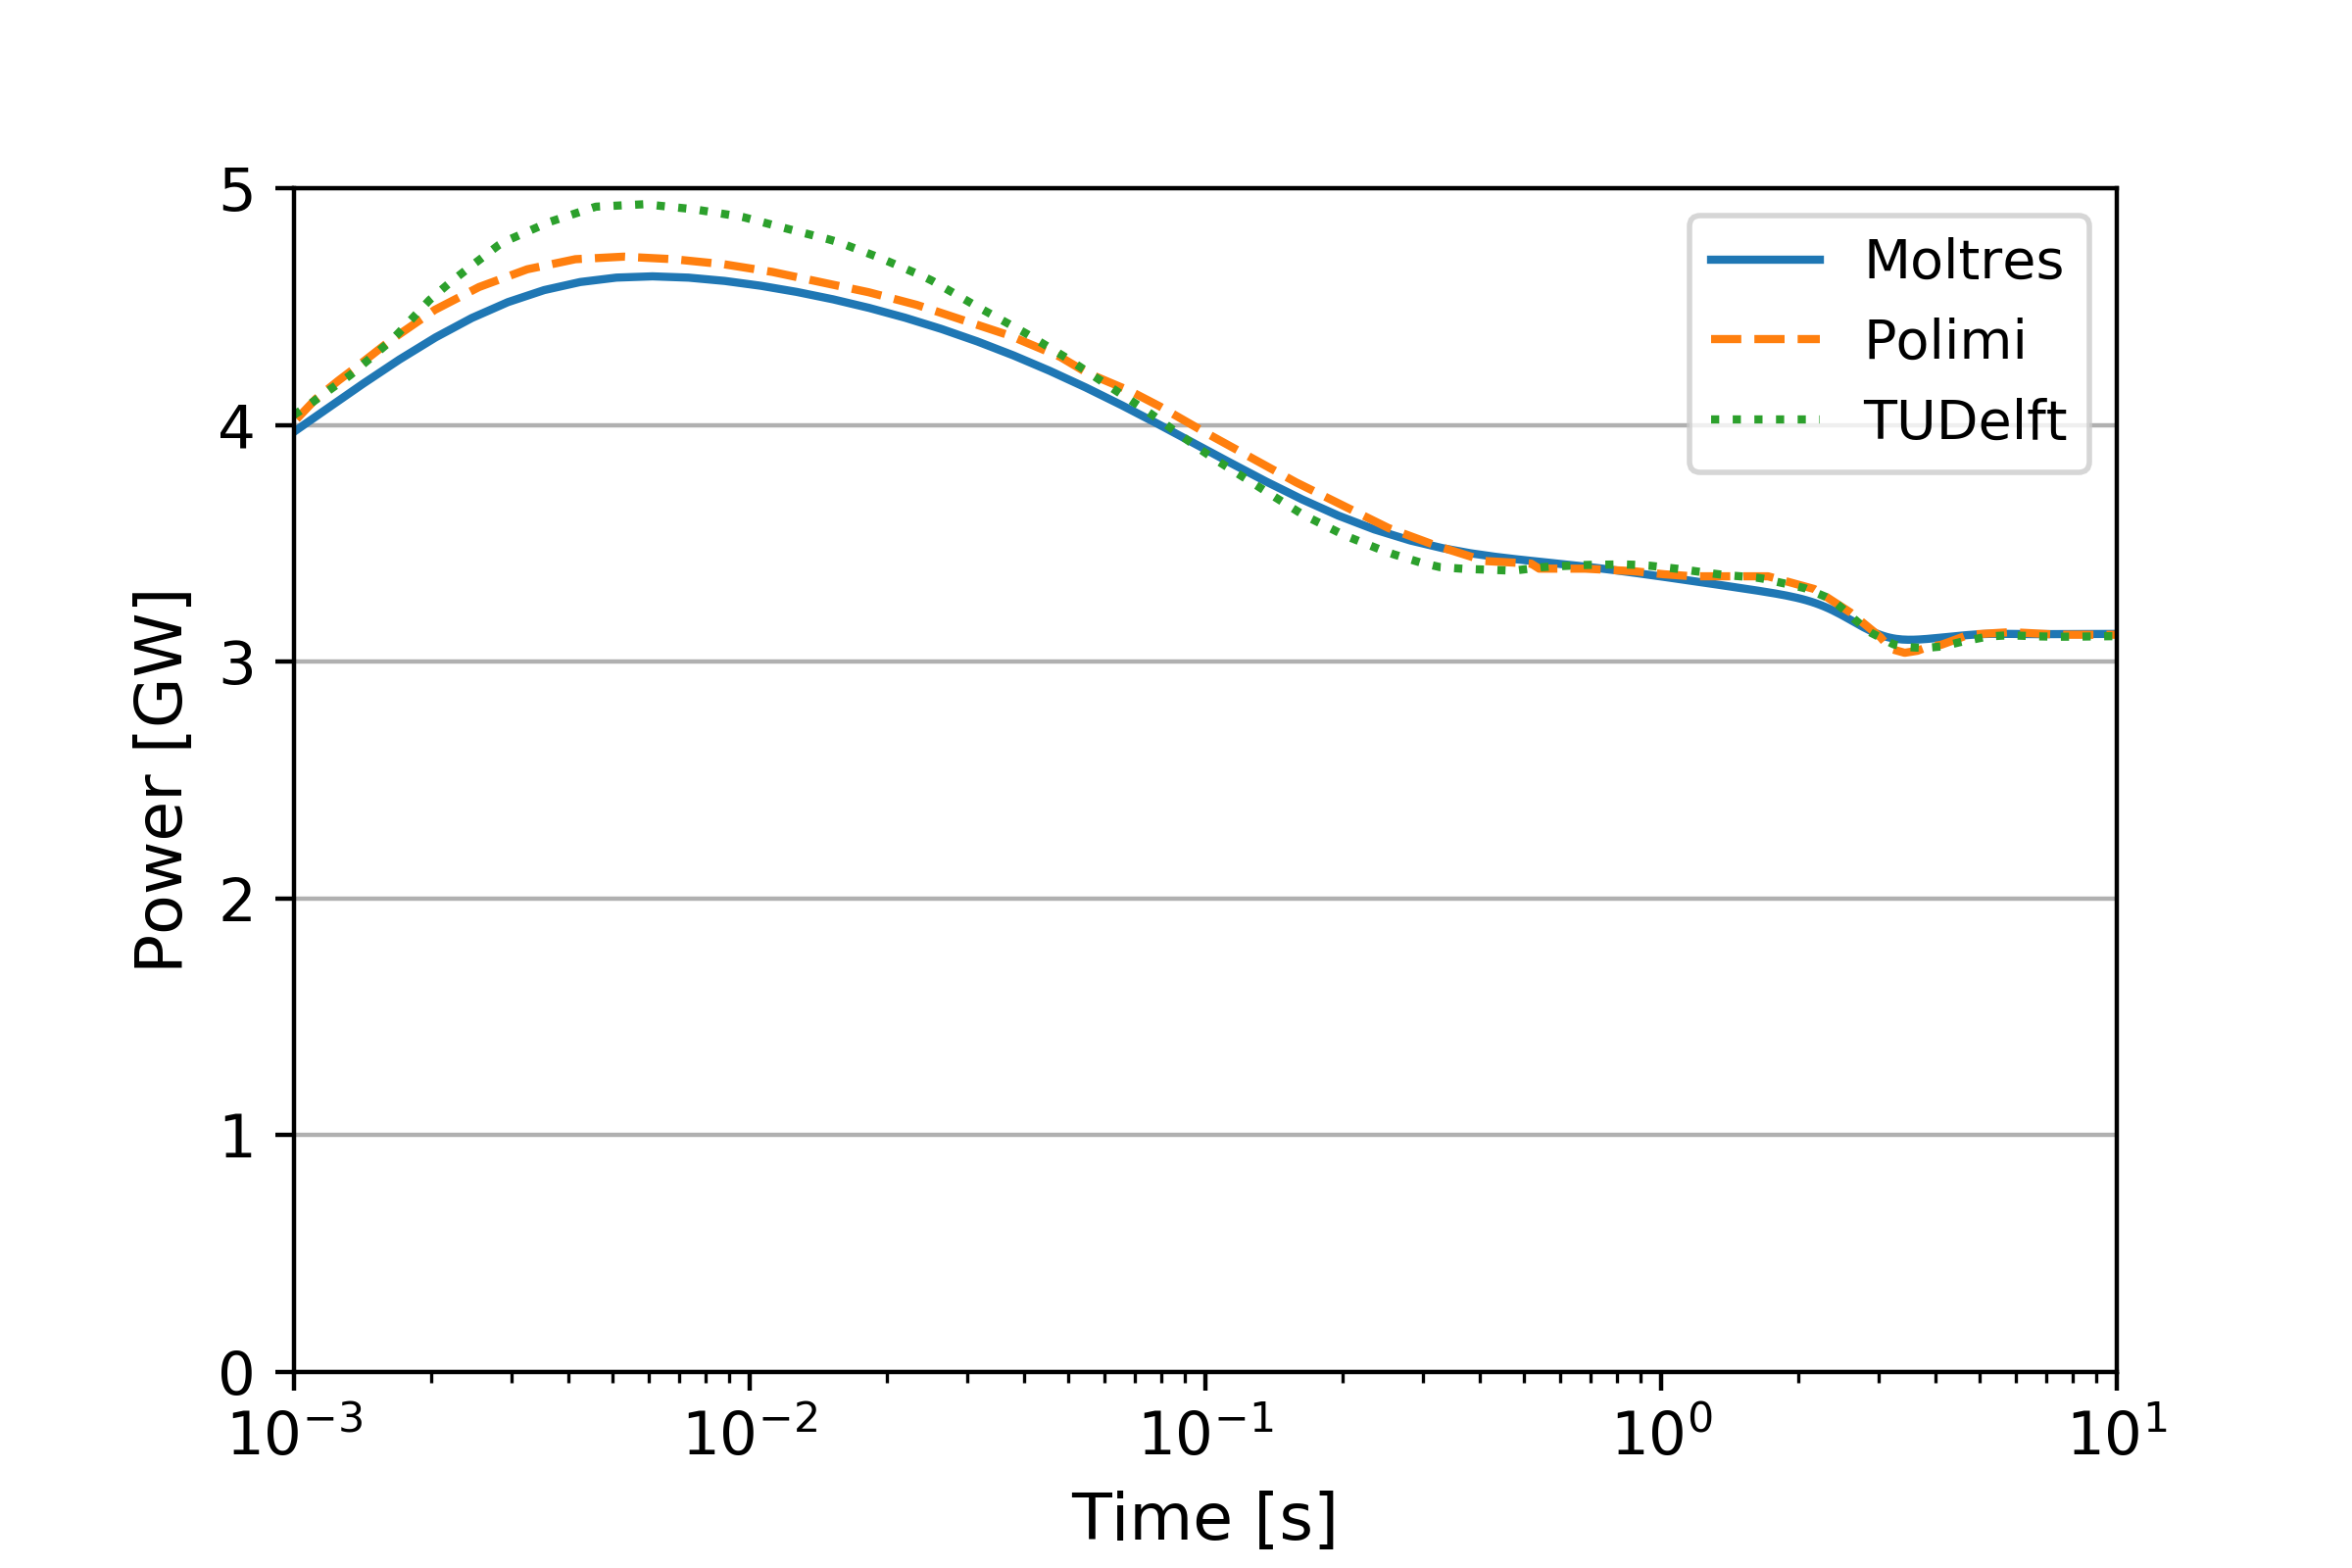
\includegraphics[width=.85\textwidth]{50pcm-heat}
    \caption{Power output following
    a 50 pcm step-wise reactivity insertion in the Moltres, Polimi, and
    TUDelft models \cite{fiorina_modelling_2014}.}
    \label{fig:50pcmheat}
%
    \centering
    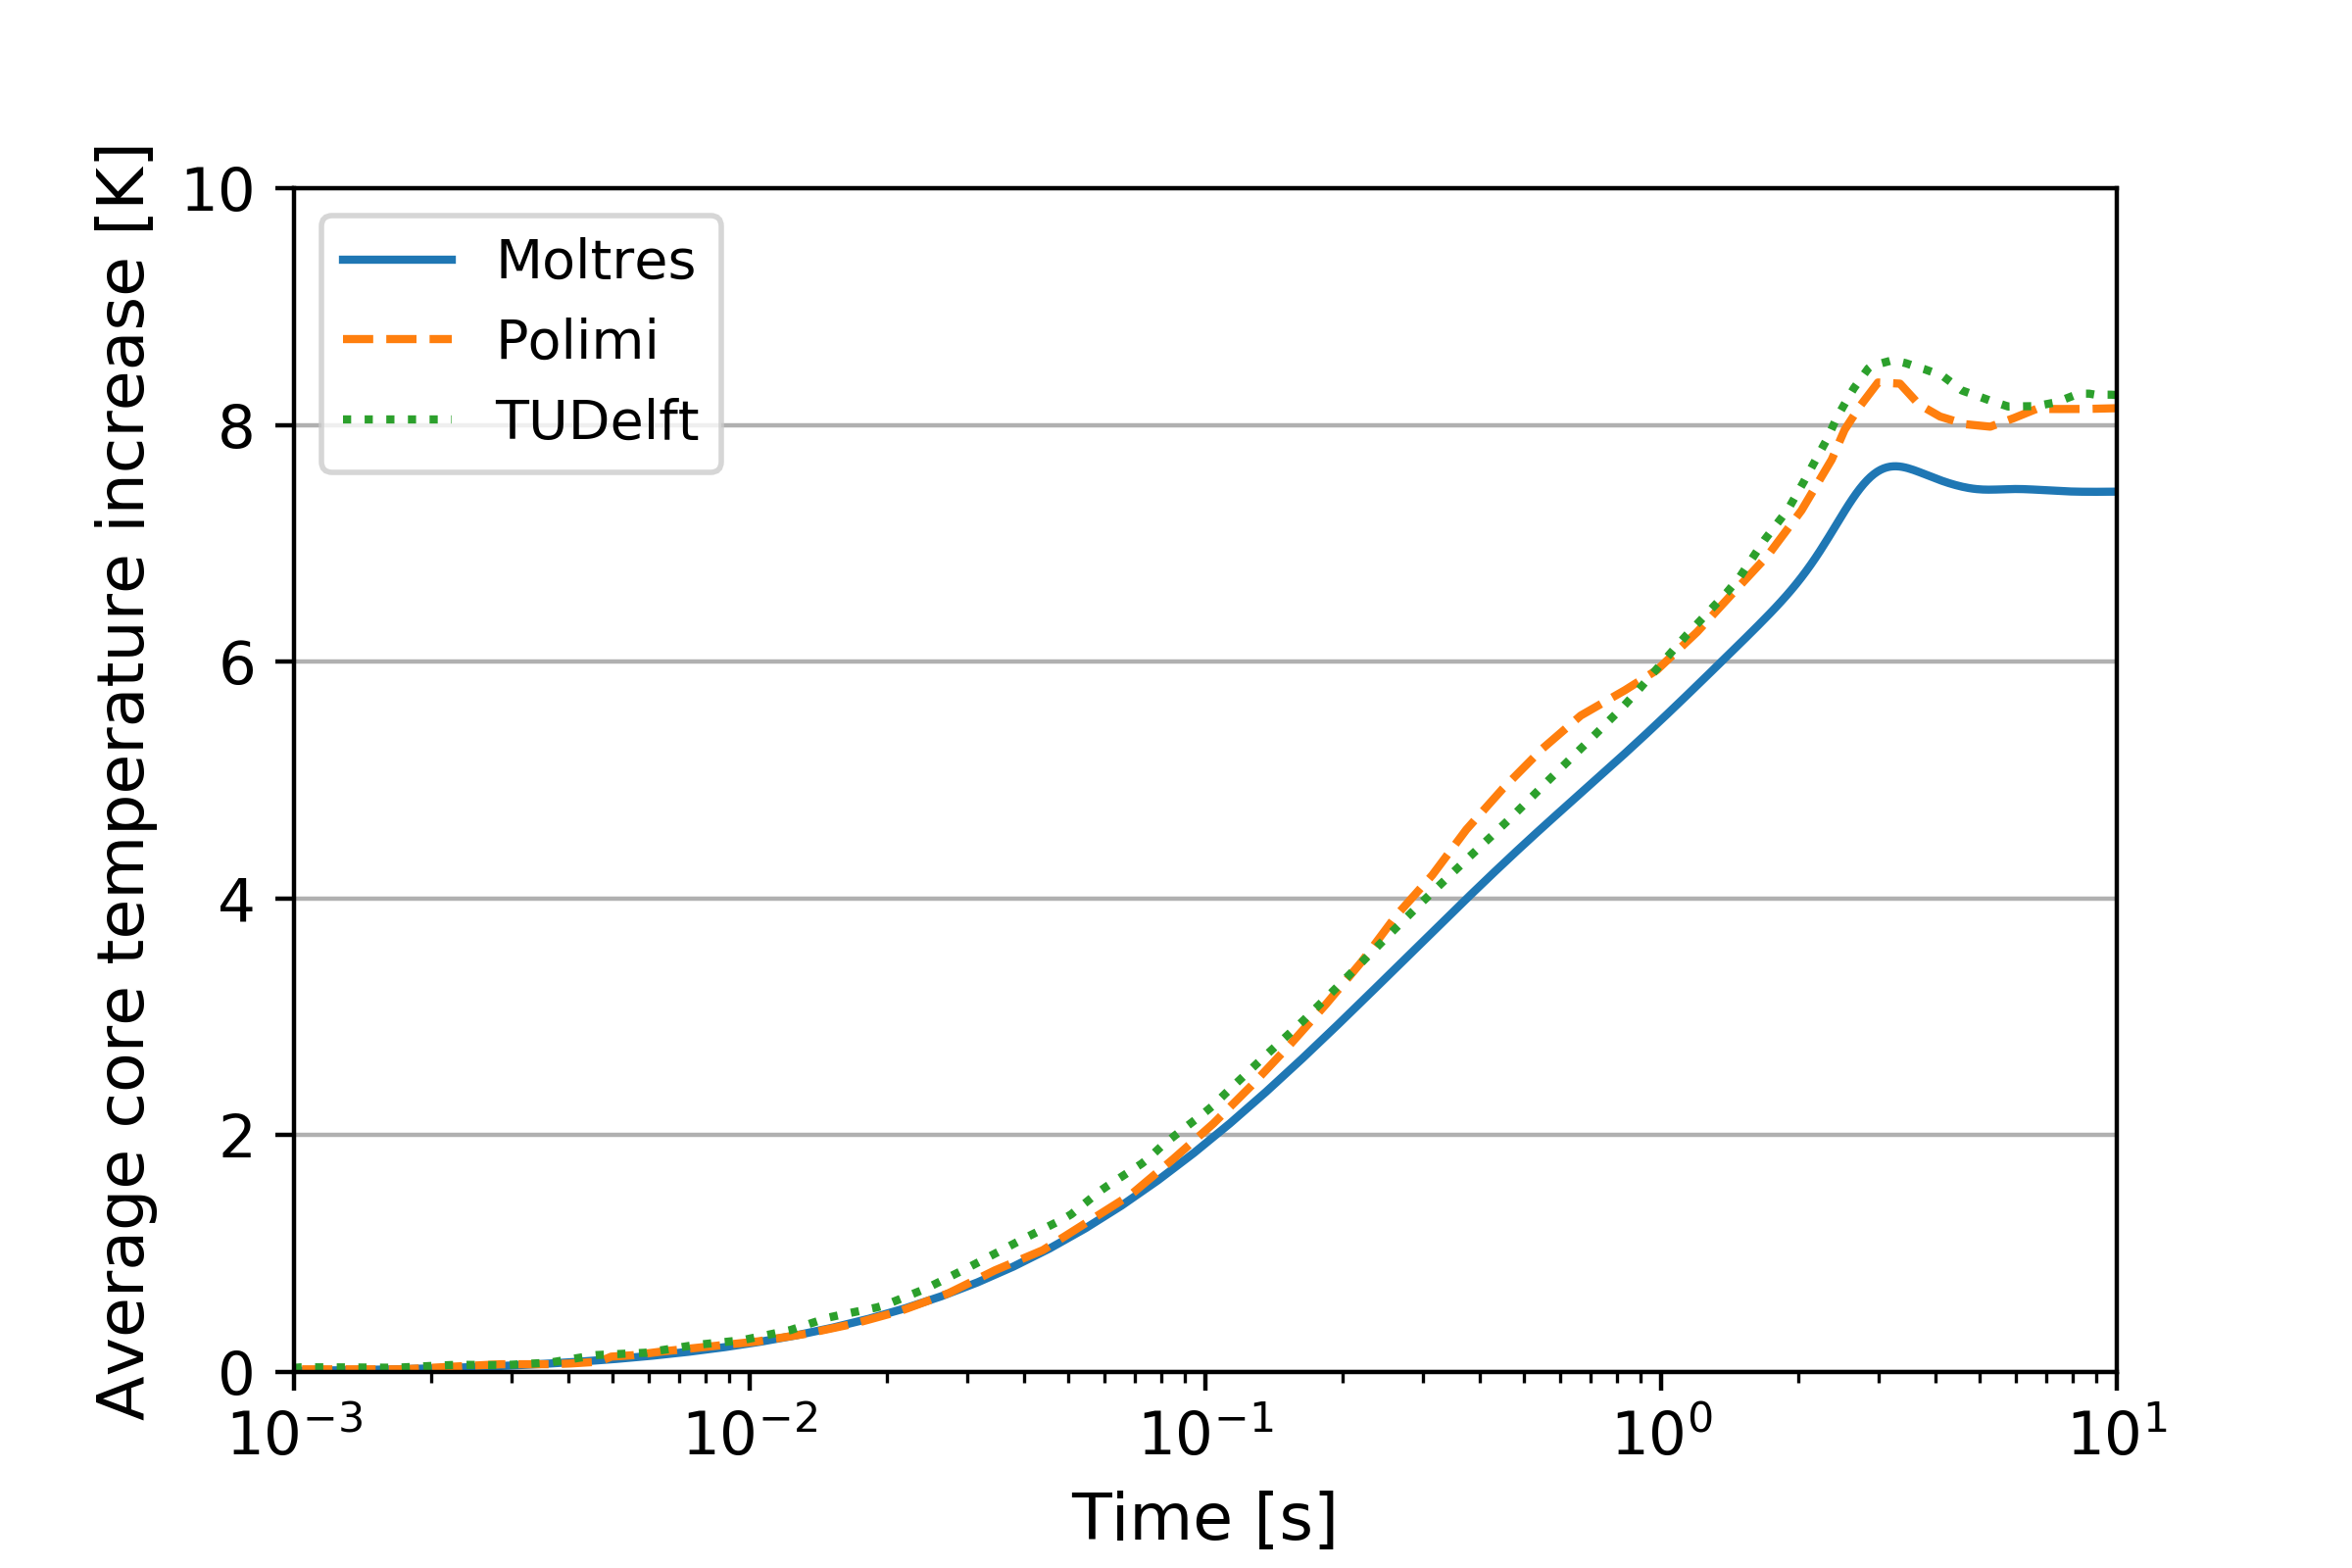
\includegraphics[width=.85\textwidth]{50pcm-temp}
    \caption{Average core temperature increase following
    a 50 pcm step-wise reactivity insertion in the Moltres, Polimi, and
    TUDelft models \cite{fiorina_modelling_2014}.}
    \label{fig:50pcmtemp}
\end{figure}

\begin{figure}[htbp!]
    \centering
    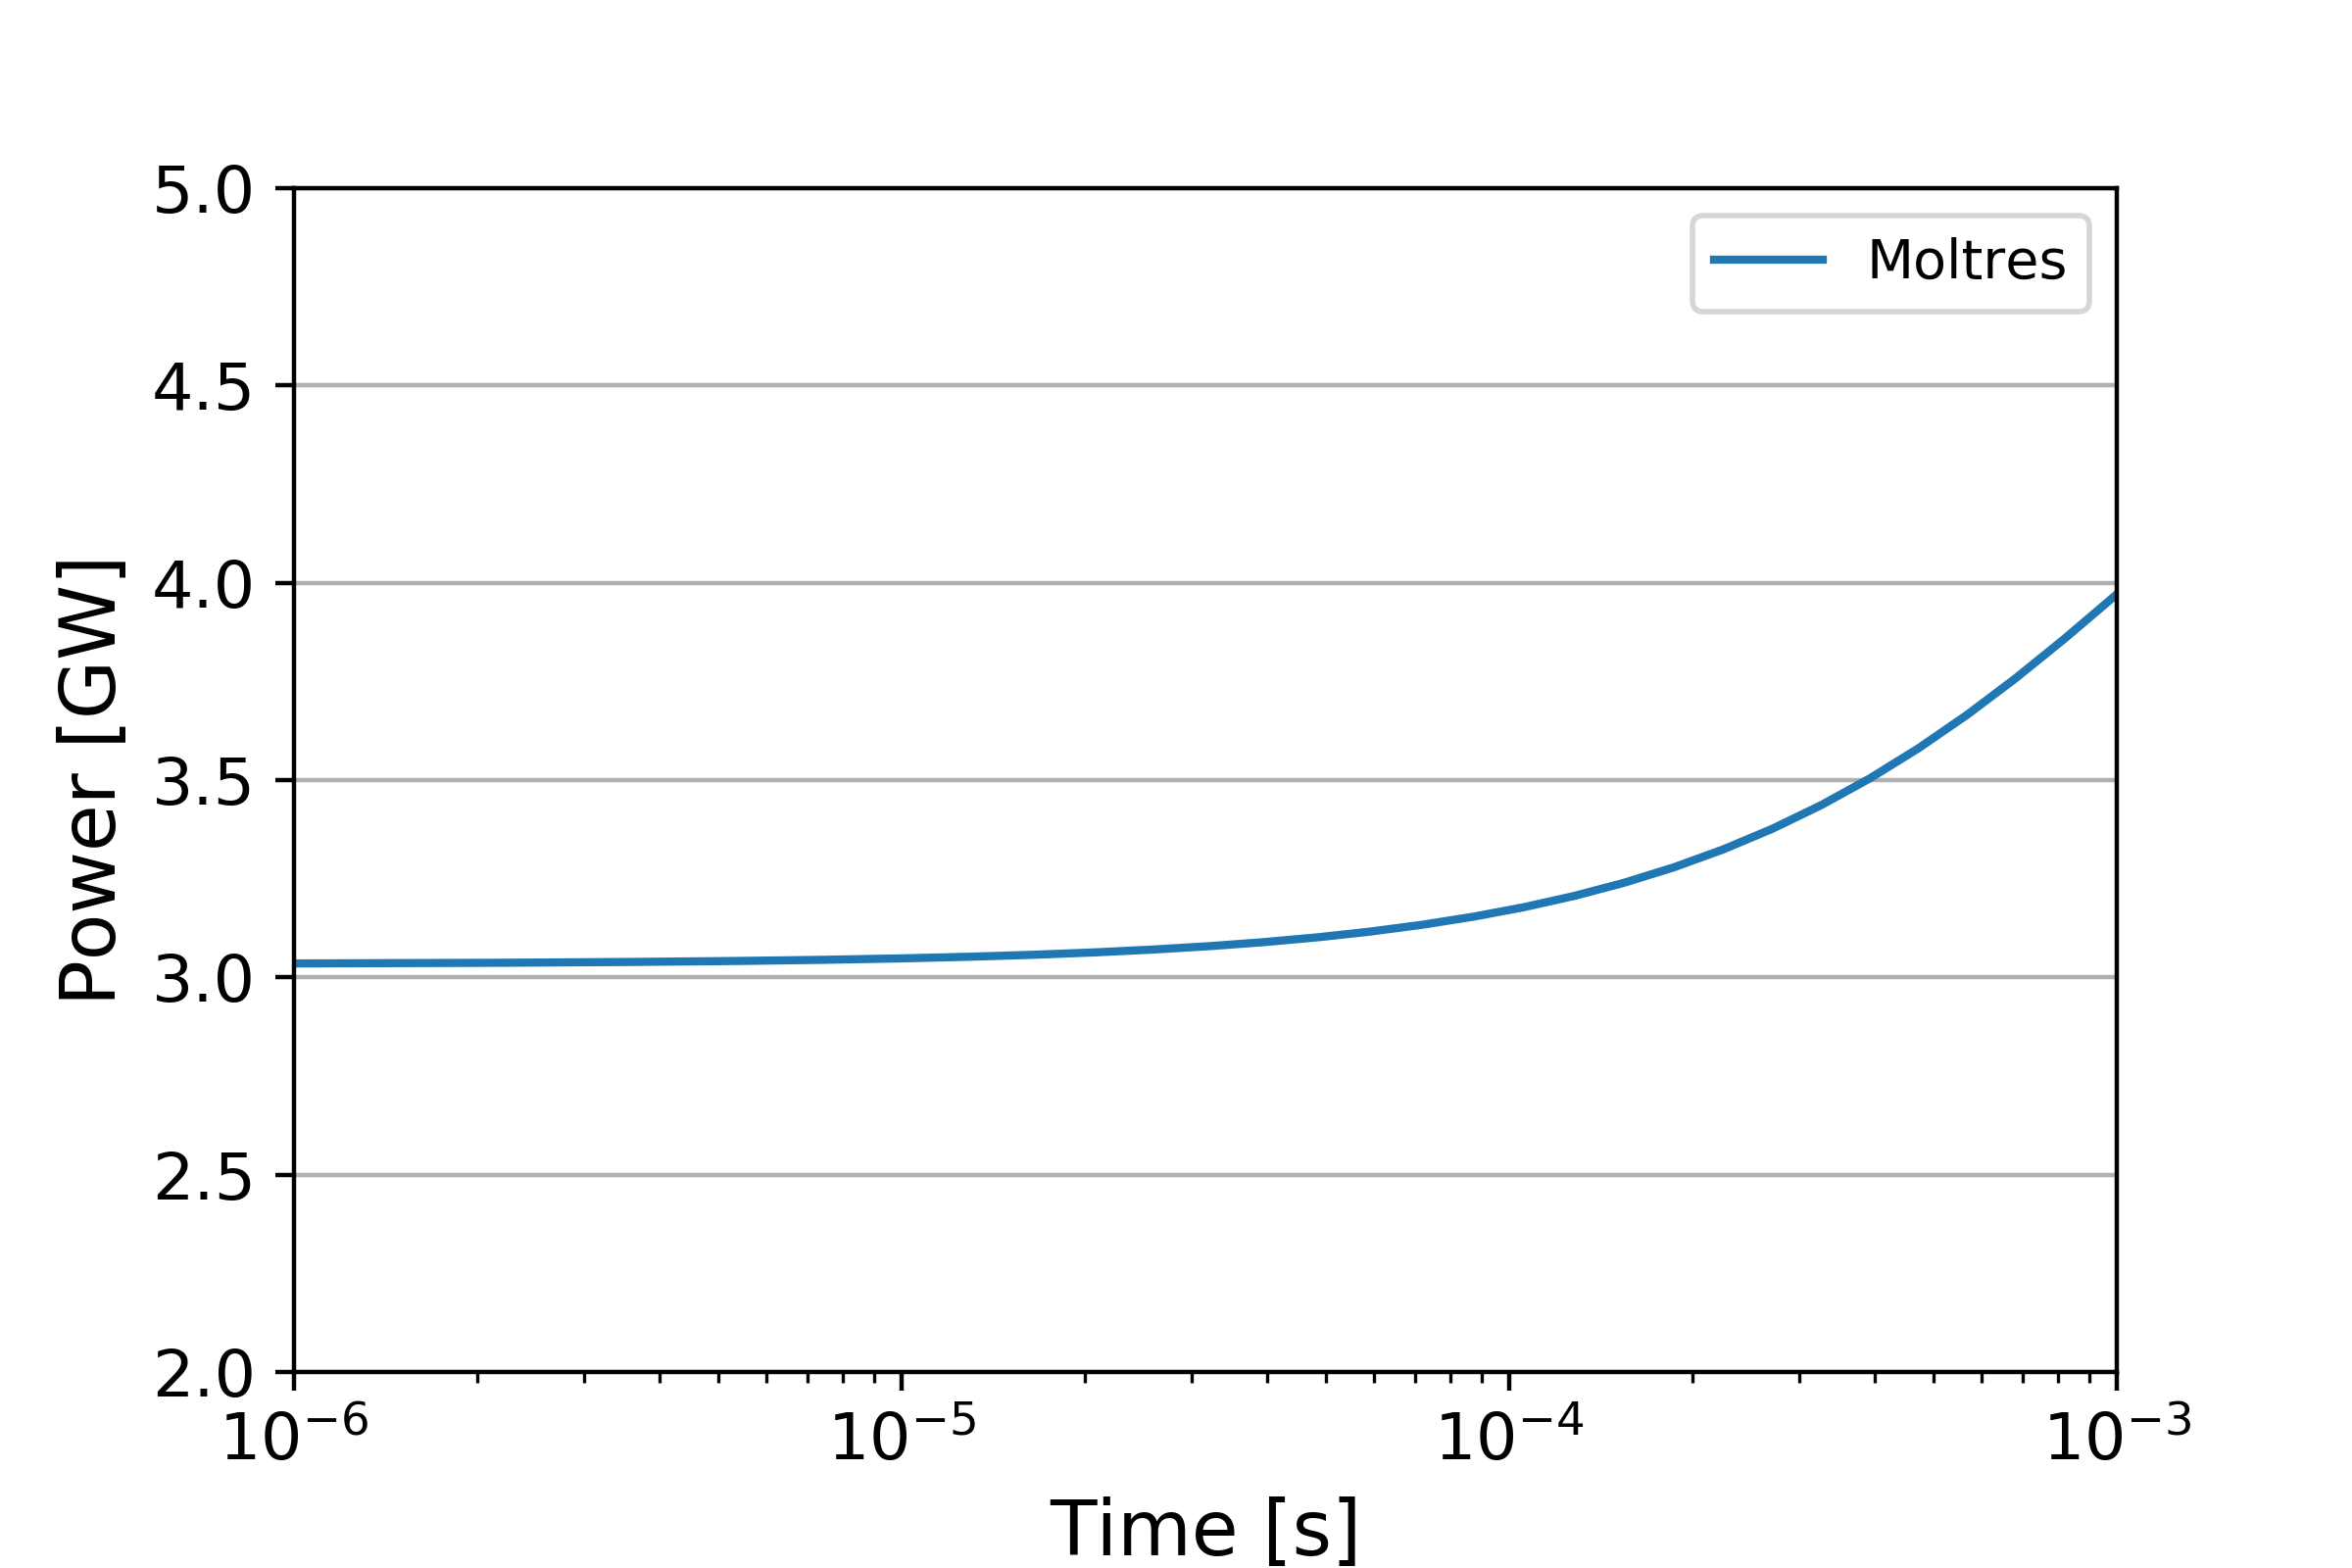
\includegraphics[width=.7\textwidth]{50pcm-jump}
    \caption{Power output during the prompt response following
    a 50 pcm step-wise reactivity insertion in the Moltres, Polimi, and
    TUDelft models \cite{fiorina_modelling_2014}.}
    \label{fig:50pcmjump}
\end{figure}

The results from Moltres show good agreement with the results from the Polimi
and TUDelft models; Moltres reproduced all of the individual features in both
plots. The magnitude of the reactor response is the most significant
difference. Moltres predicts a smaller peak in the power output and a smaller
overall increase in the average core temperature mainly due to the
more negative temperature reactivity coefficient in Moltres than in the Polimi
and TUDelft models. The temperature reactivity coefficient $\alpha_T$ in
Moltres is $-7.184$ pcm K$^{-1}$ (Table \ref{table:alpha}), as opposed to
approximately $-6.5$ pcm K$^{-1}$ within the relevant temperature range in the
Polimi and TUDelft models. Therefore, the results show a smaller temperature
increase in the Moltres model for the same reactivity insertion. Multiplying
the average
core temperature increase at $t=10$ s with $\alpha_T$ gives us $-7.184$ pcm
K$^{-1} \times 7.46$ K $= -53.6$ pcm, which is approximately equal to the 50
pcm reactivity insertion.

\begin{figure}[htbp!]
    \centering
    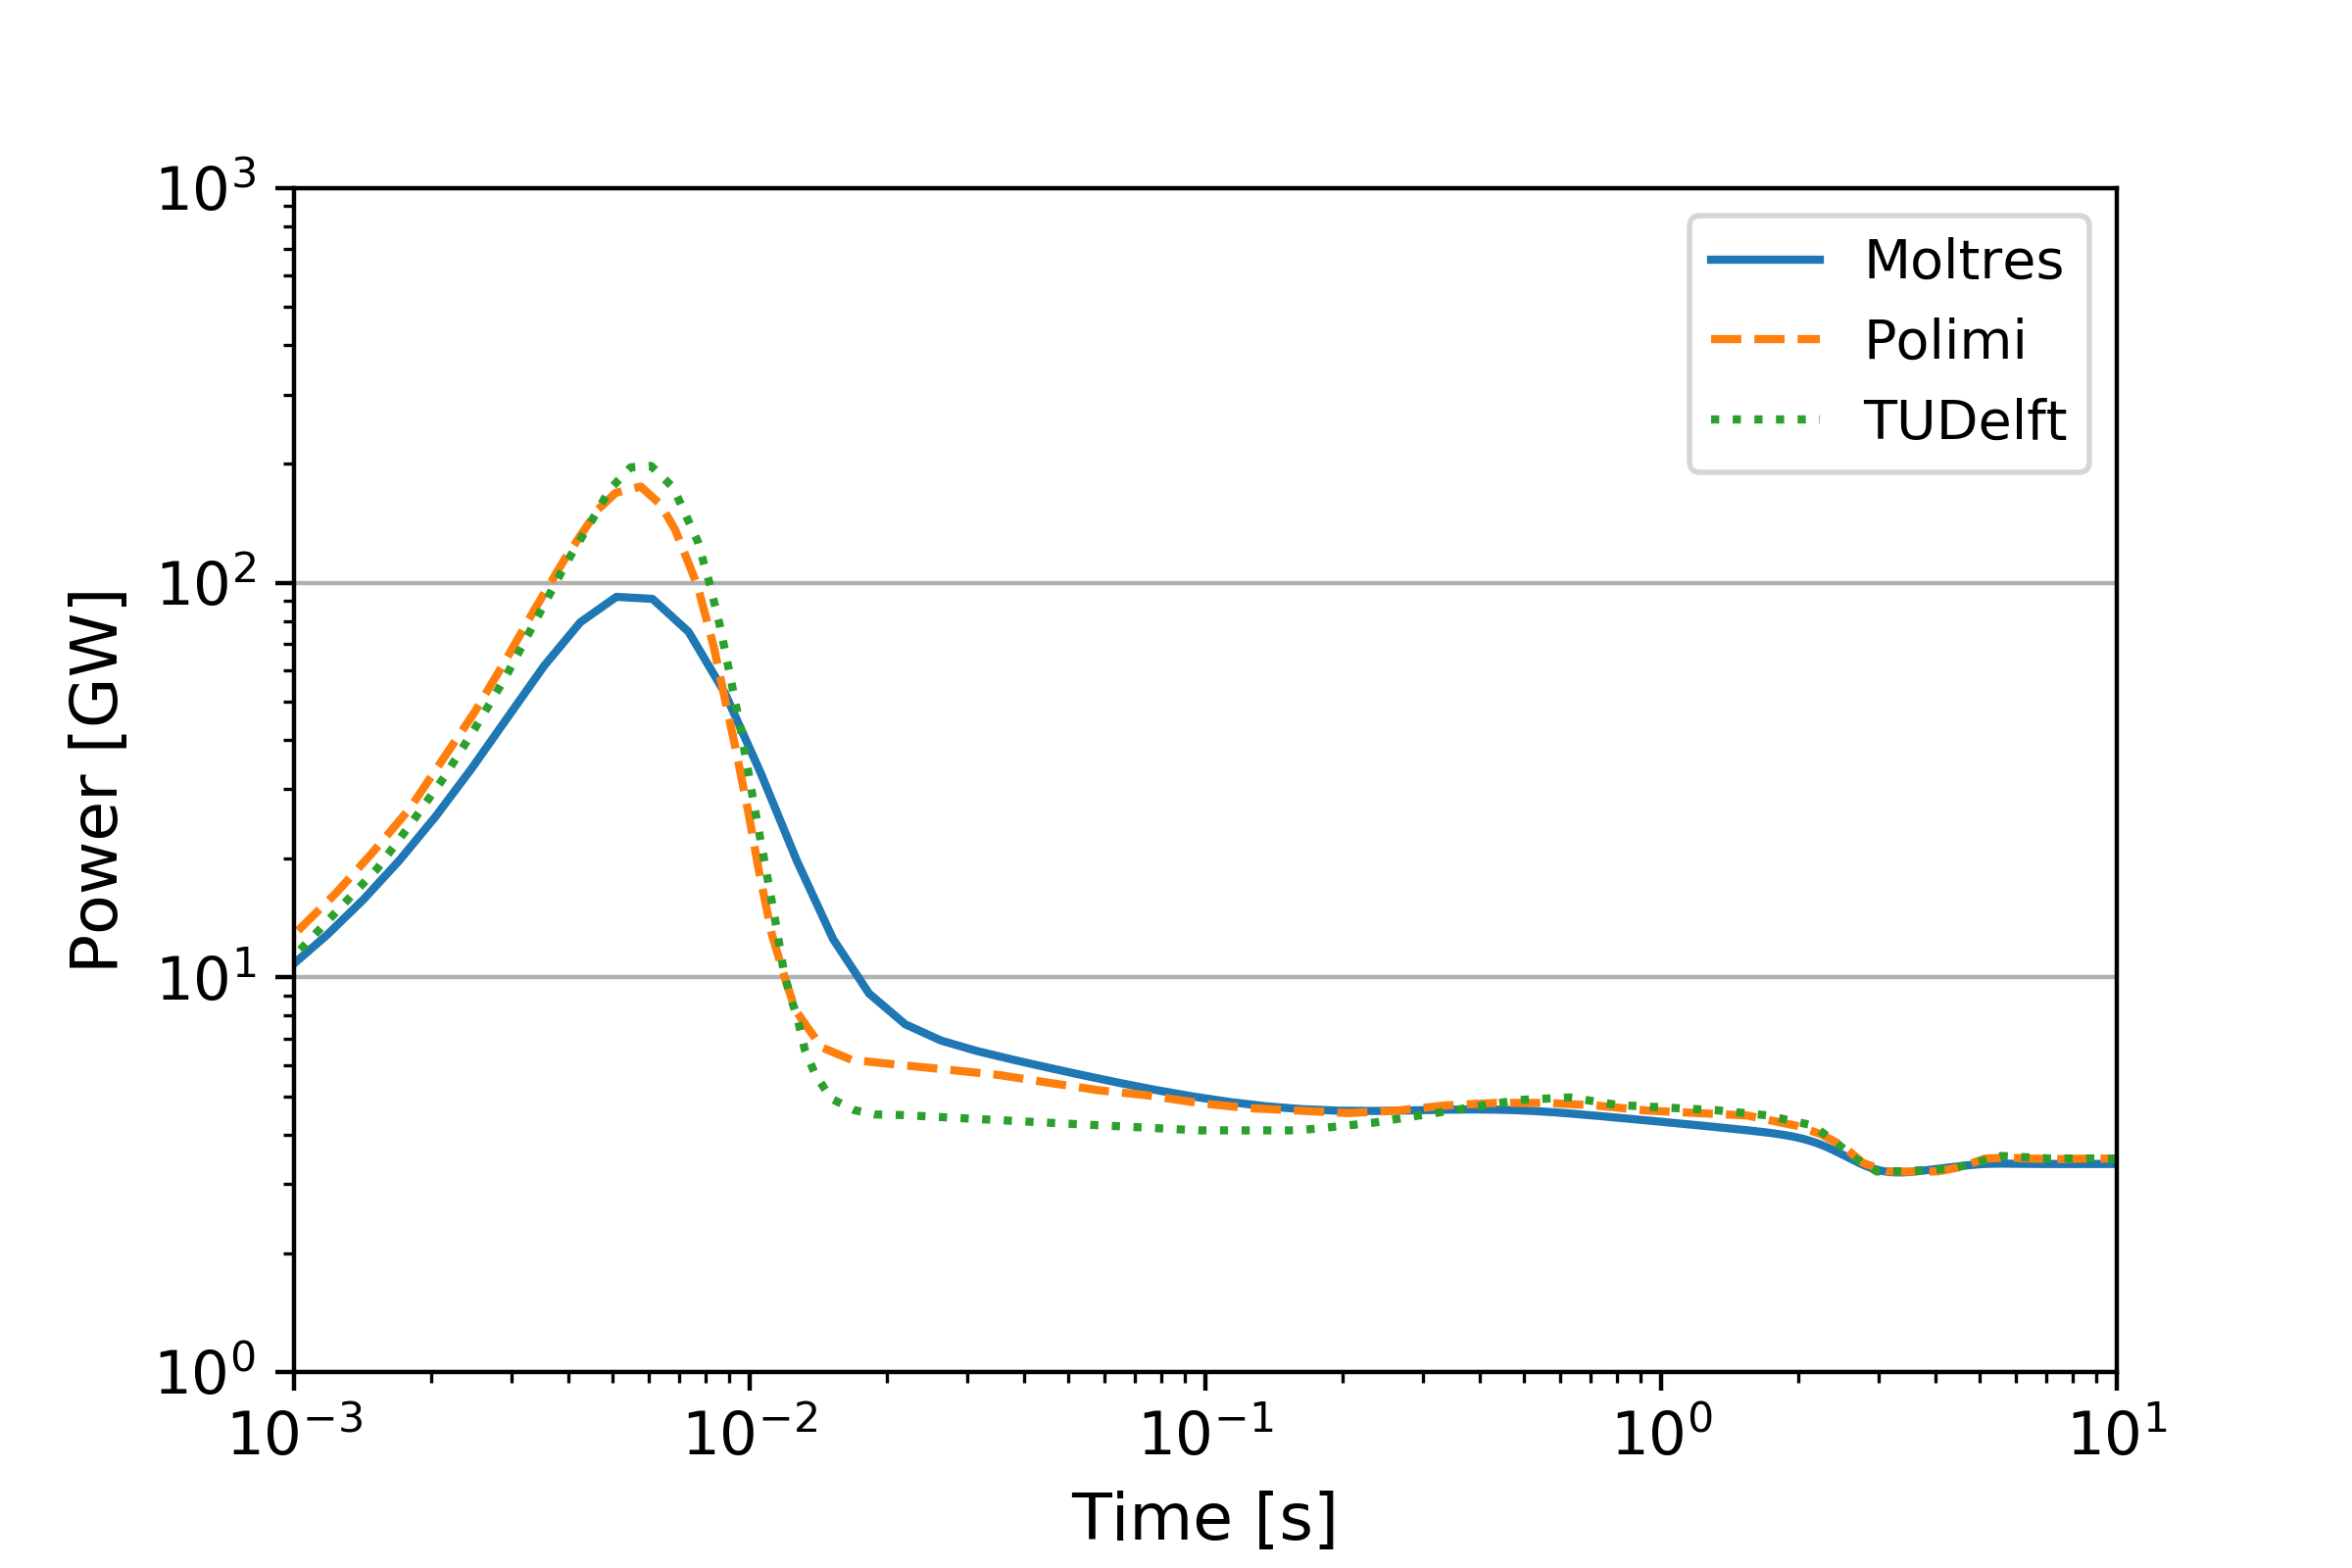
\includegraphics[width=.85\textwidth]{200pcm-heat}
    \caption{Power output following
    a 200 pcm step-wise reactivity insertion in the Moltres, Polimi, and
    TUDelft models \cite{fiorina_modelling_2014}.}
    \label{fig:200pcmheat}
%
    \centering
    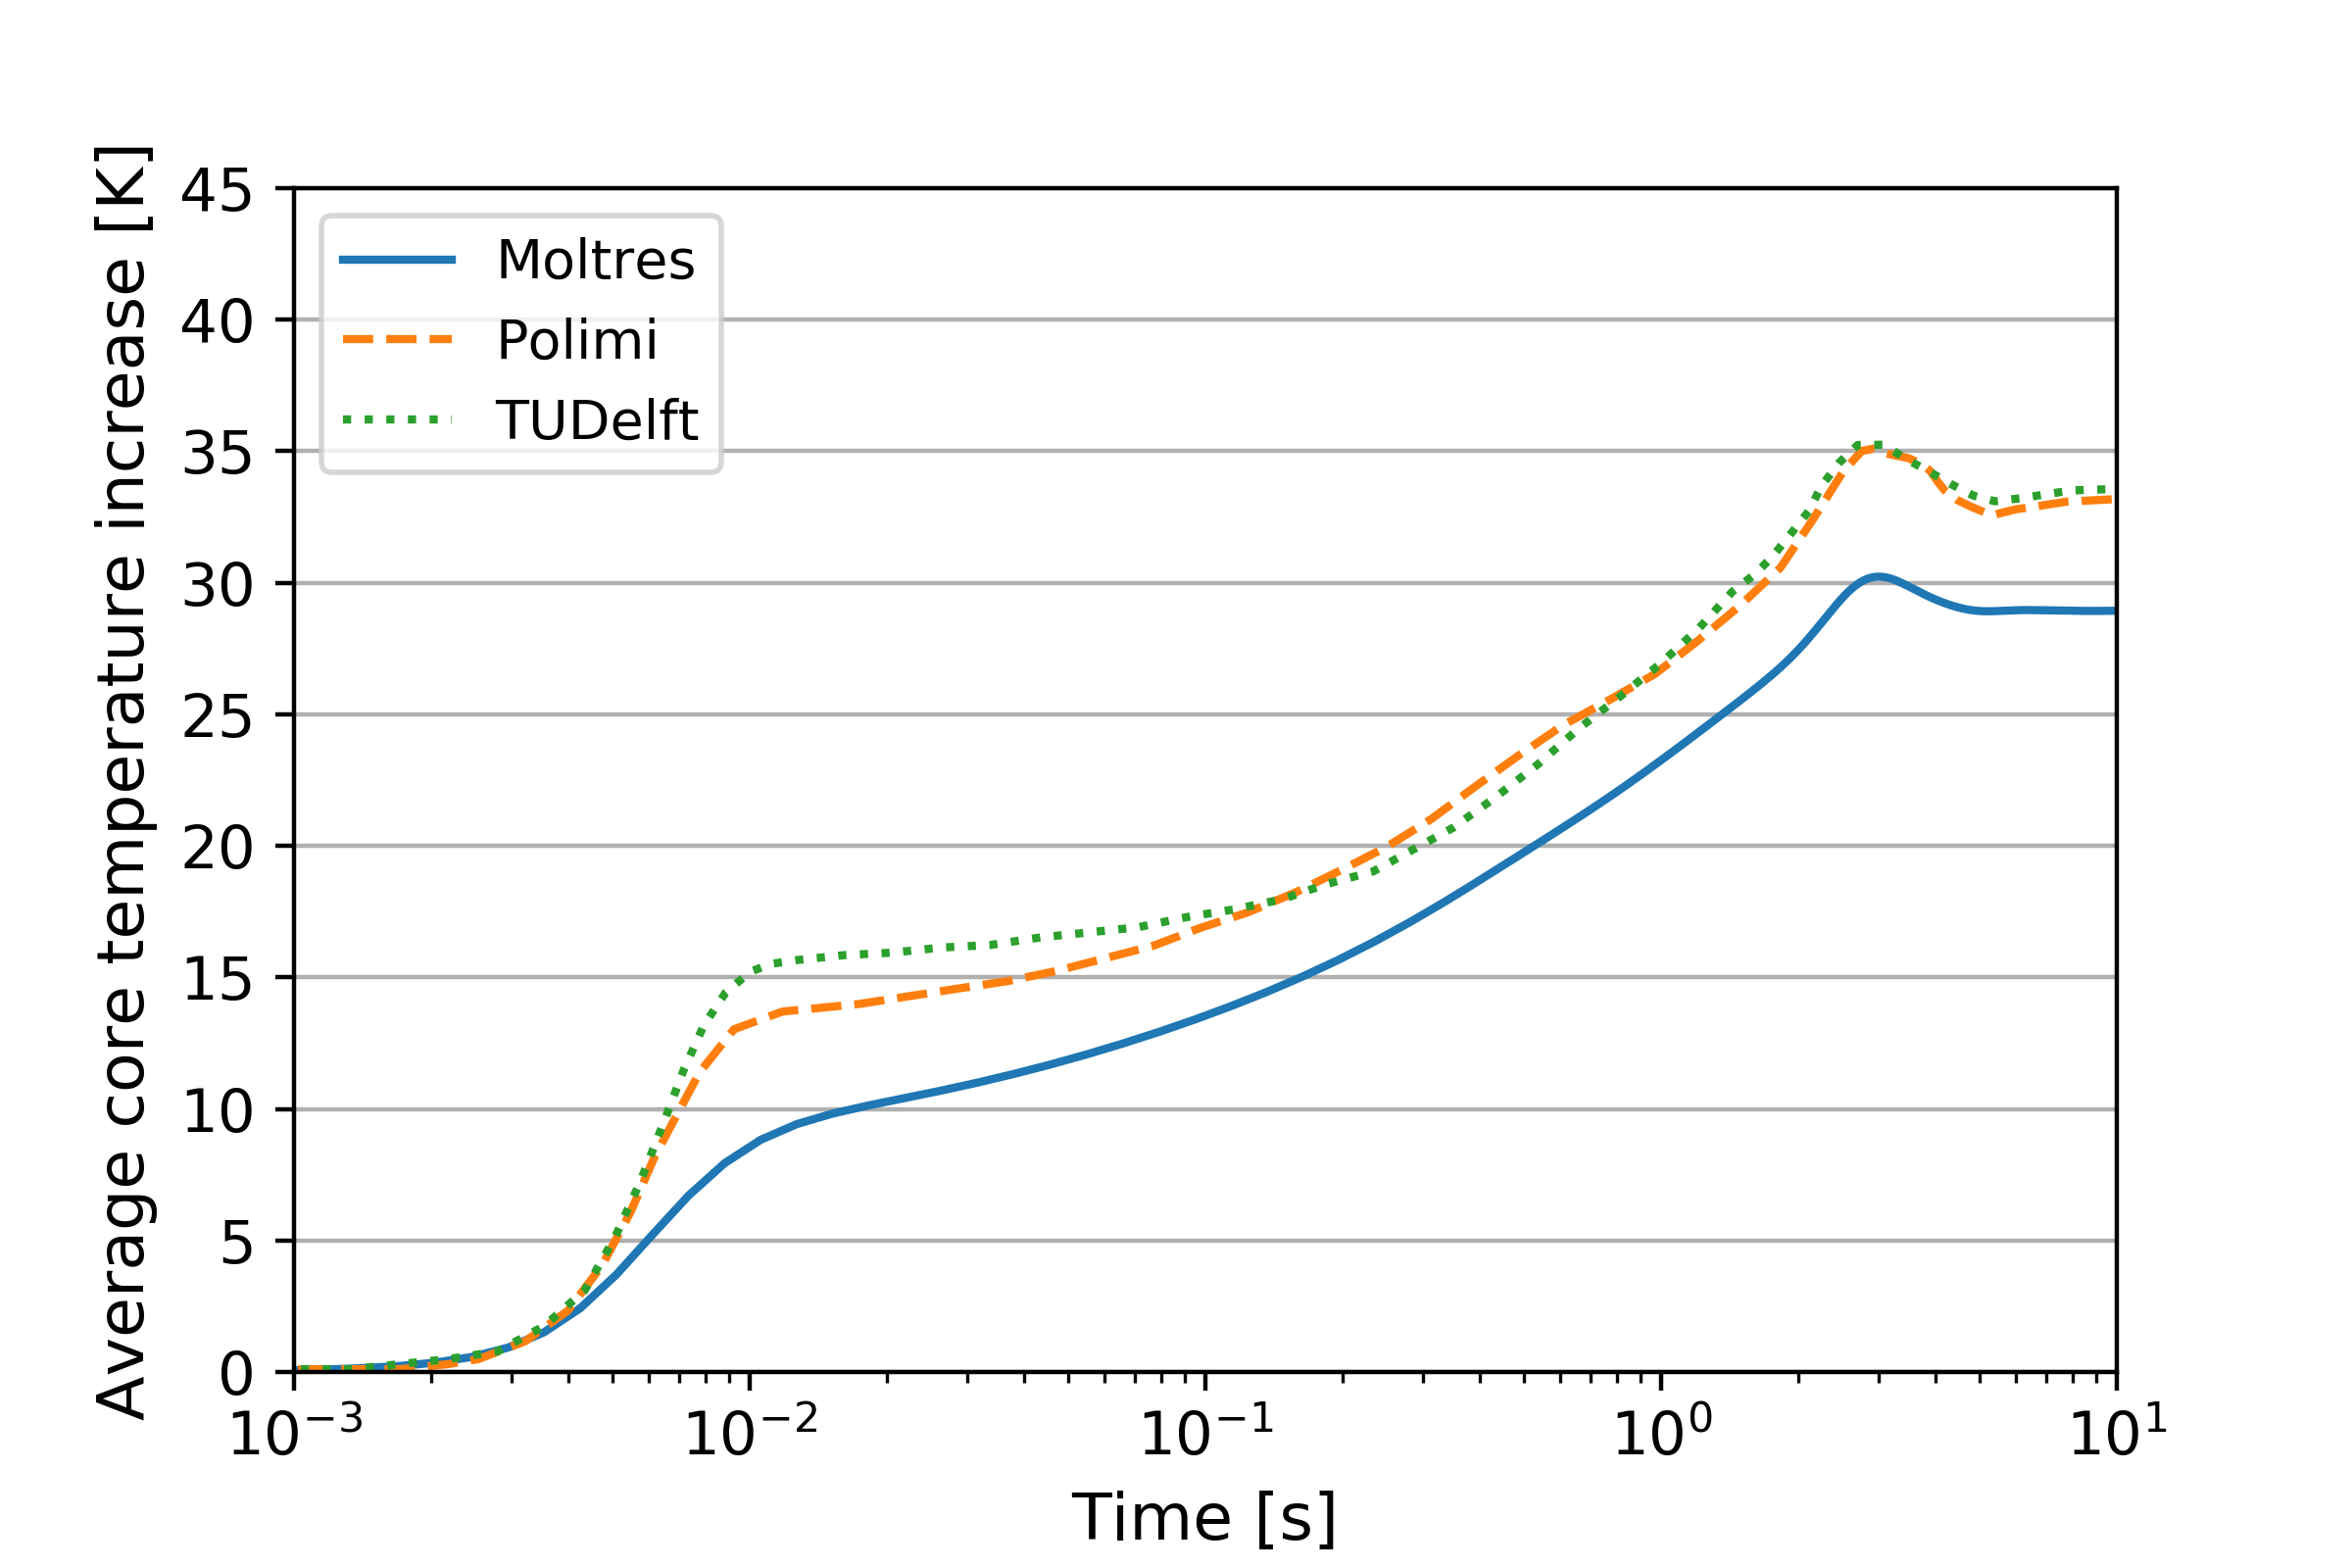
\includegraphics[width=.85\textwidth]{200pcm-temp}
    \caption{Average core temperature increase following
    a 200 pcm step-wise reactivity insertion in the Moltres, Polimi, and
    TUDelft models \cite{fiorina_modelling_2014}.}
    \label{fig:200pcmtemp}
\end{figure}

The results for the 200 pcm reactivity insertion scenario show similar trends
to the 50 pcm case. The greater reactivity insertion elicits a stronger
prompt response in the power output which peaks at 92.1 GW. The average core
temperature increases much more rapidly and subsequently triggers a sharper
drop in power output. This results in the clearer distinction in the rate of
core temperature increase before and after $t=0.01$ s. In this transient, we
also observe greater deviation between Moltres and the other models arising
from the differences in the temperature reactivity coefficients. Overall,
Moltres' results show good agreement with the Polimi and TUDelft results.
The differences arise mainly due to the differences in the temperature
reactivity coefficients.

\clearpage

\section{Unprotected Loss of Heat Sink}

An unprotected loss of heat sink accident can occur when the pumps in the
intermediate loop fail. The heat exchangers would then lose most of their
cooling capabilities. This work followed Fiorina et al.'s approach in assuming
that the cooling from the heat exchangers decreases exponentially with a time
constant of 1 s and all other parameters held constant
\cite{fiorina_modelling_2014}. As mentioned in the Chapter \ref{chap:ss}, we
will present two sets of results for this transient: 1) without decay heat
modeling, and 2) with decay heat modeling.

\subsection{Without Decay Heat} \label{sec:wodecayheat}

Figures \ref{fig:lohsheat} and \ref{fig:lohstemp} show the power output and
average core temperature increase during the unprotected loss of heat sink
transient in the Moltres, Polimi, and TUDelft models without decay heat
modeling. The power output and average core temperature show little change in
the first two seconds as it takes approximately that amount of time for the
partially cooled salt to migrate to the center of the core. At $t=2$ s, we
observe a sharp spike in average core temperature and a corresponding drop
in power output. The presence of delayed neutron precursors (DNPs) from the
steady-state operating conditions momentarily halt the increase in temperature
at around $t=5$ s. The average core temperature continues to rise while the
power output falls through the rest of the transient.

The results from Moltres show good agreement with the results from the Polimi
and TUDelft. Moltres reproduced all of the trends in the Polimi
and TUDelft models. The temporary halt in the temperature increase occurs at
a lower average core temperature for Moltres than the other two models. This
is likely due to the difference in the temperature reactivity coefficient
discussed in the reactivity insertion results; a smaller increase in
the average core temperature produces the same decrease in power output.

\begin{figure}[htbp!]
    \centering
    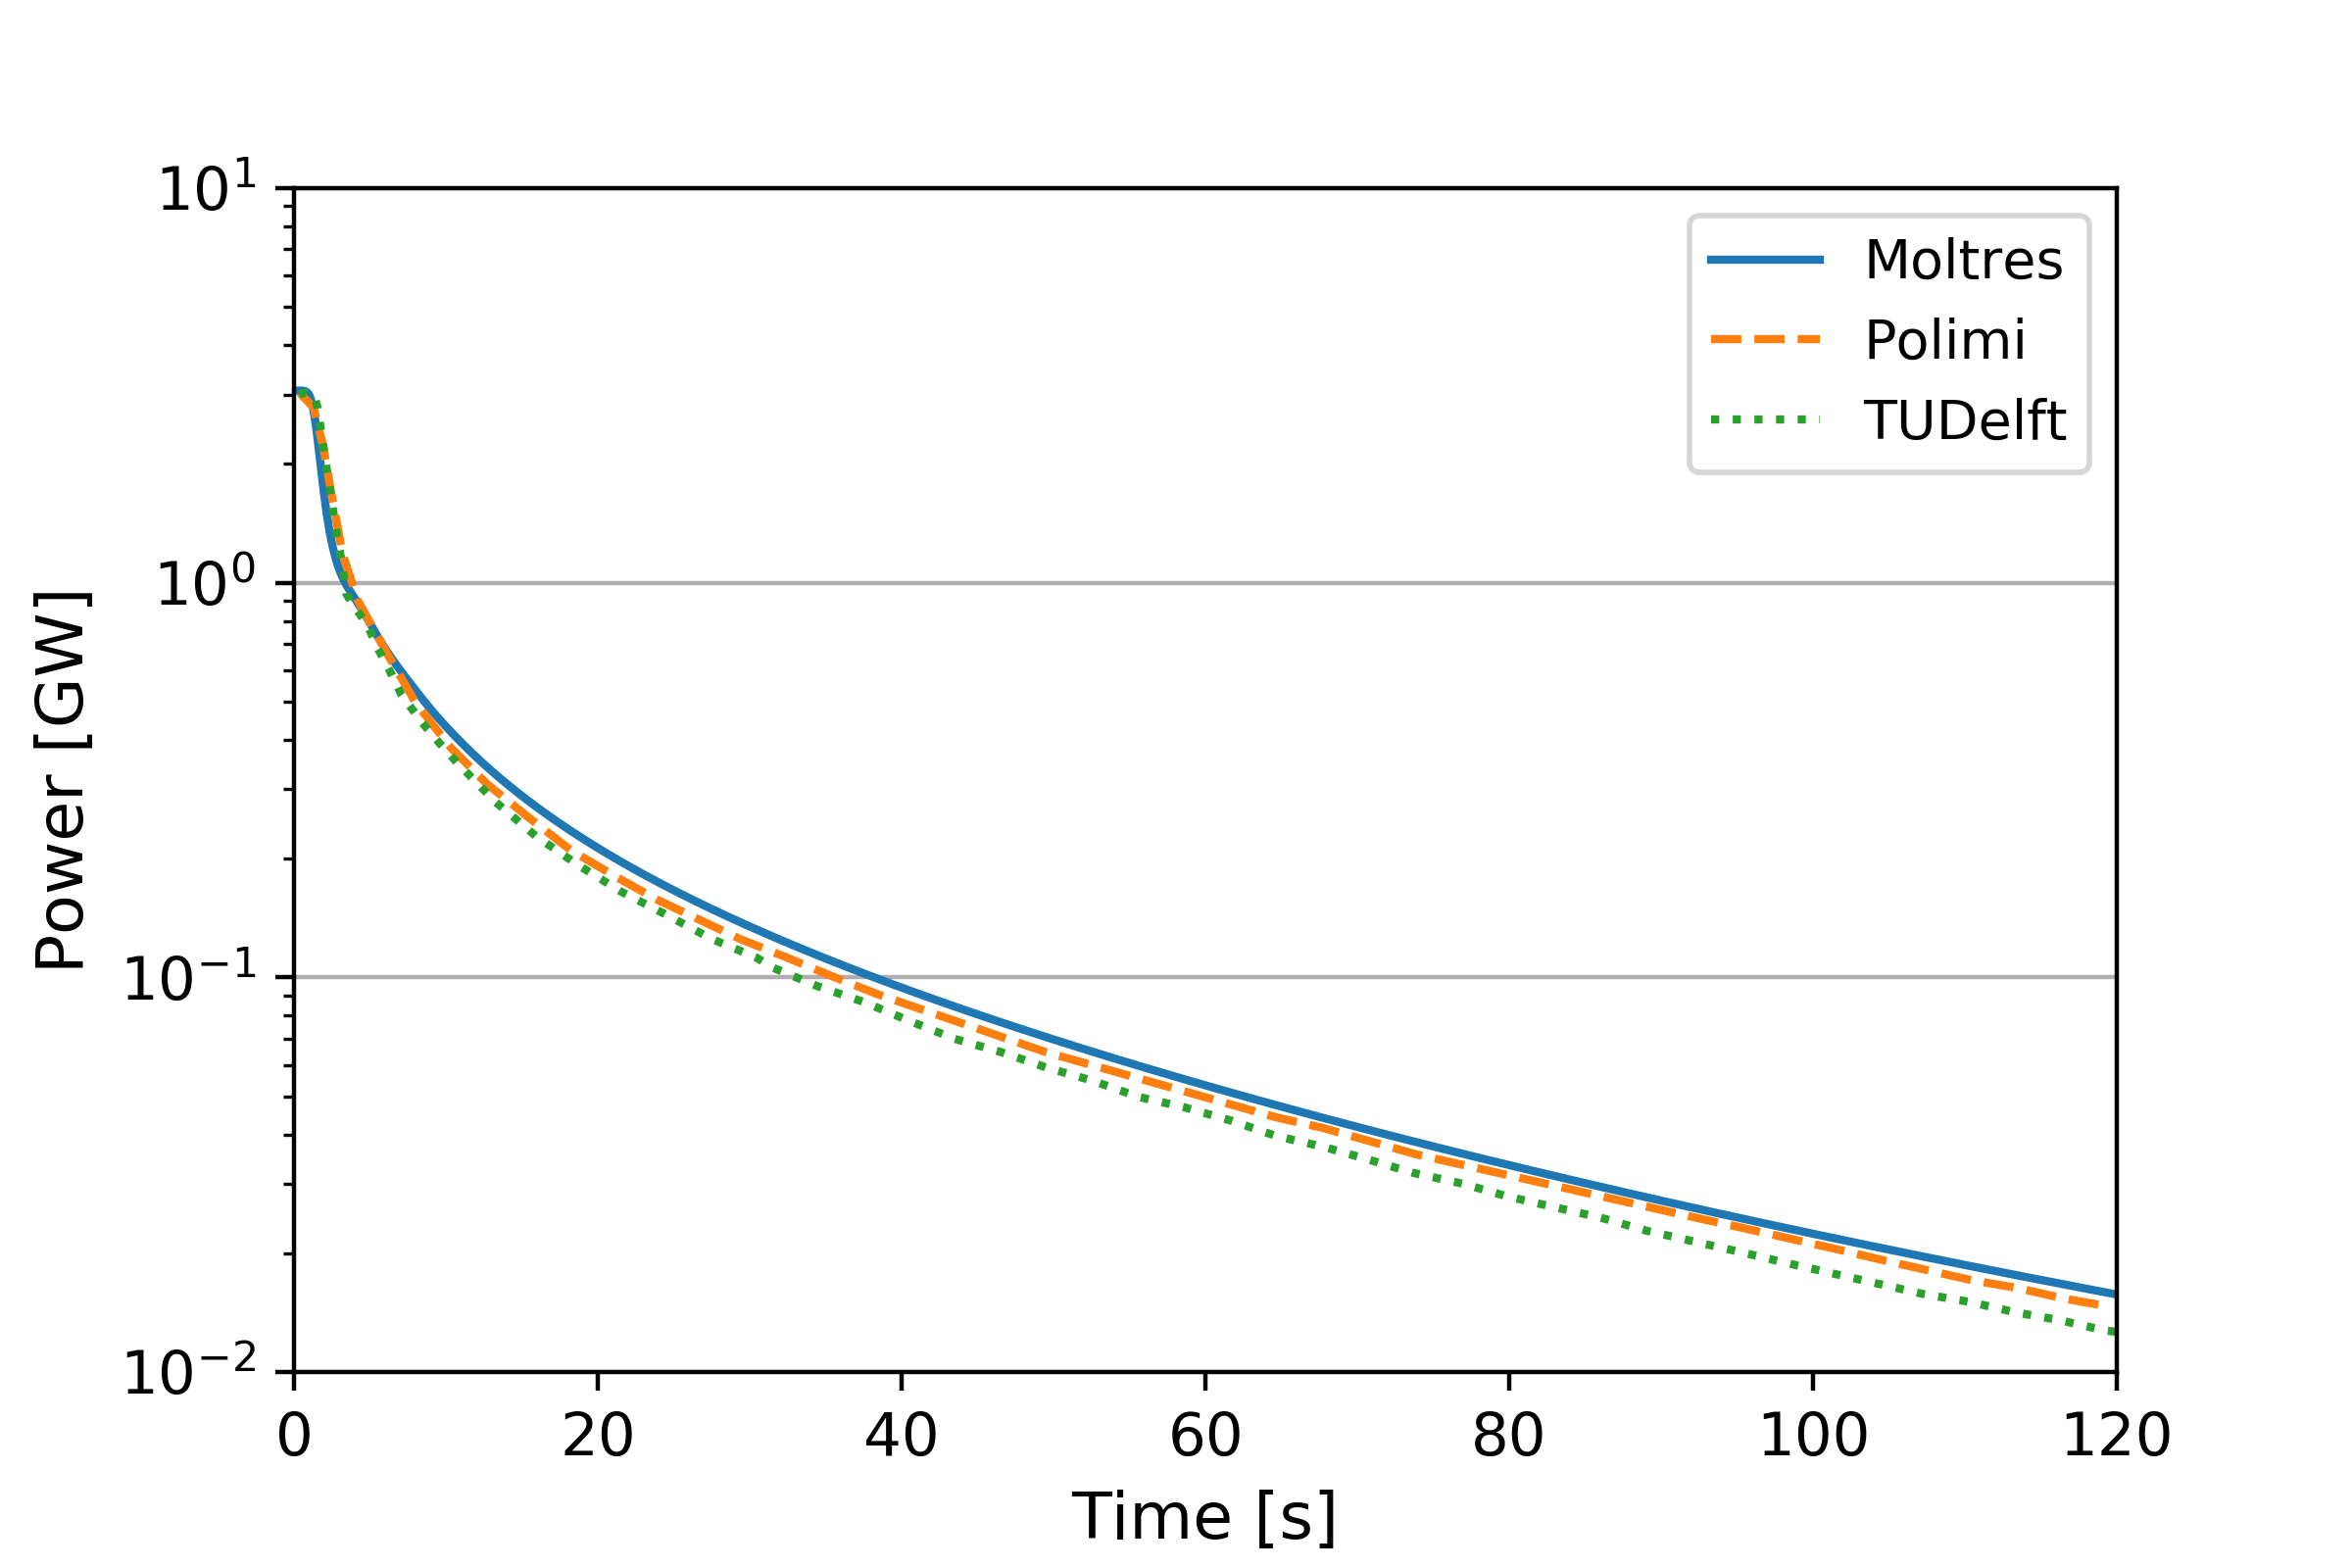
\includegraphics[width=.85\textwidth]{lohs-heat}
    \caption{Power output during
    an unprotected loss of heat sink transient in the Moltres, Polimi, and
    TUDelft models \cite{fiorina_modelling_2014} without decay heat.}
    \label{fig:lohsheat}
    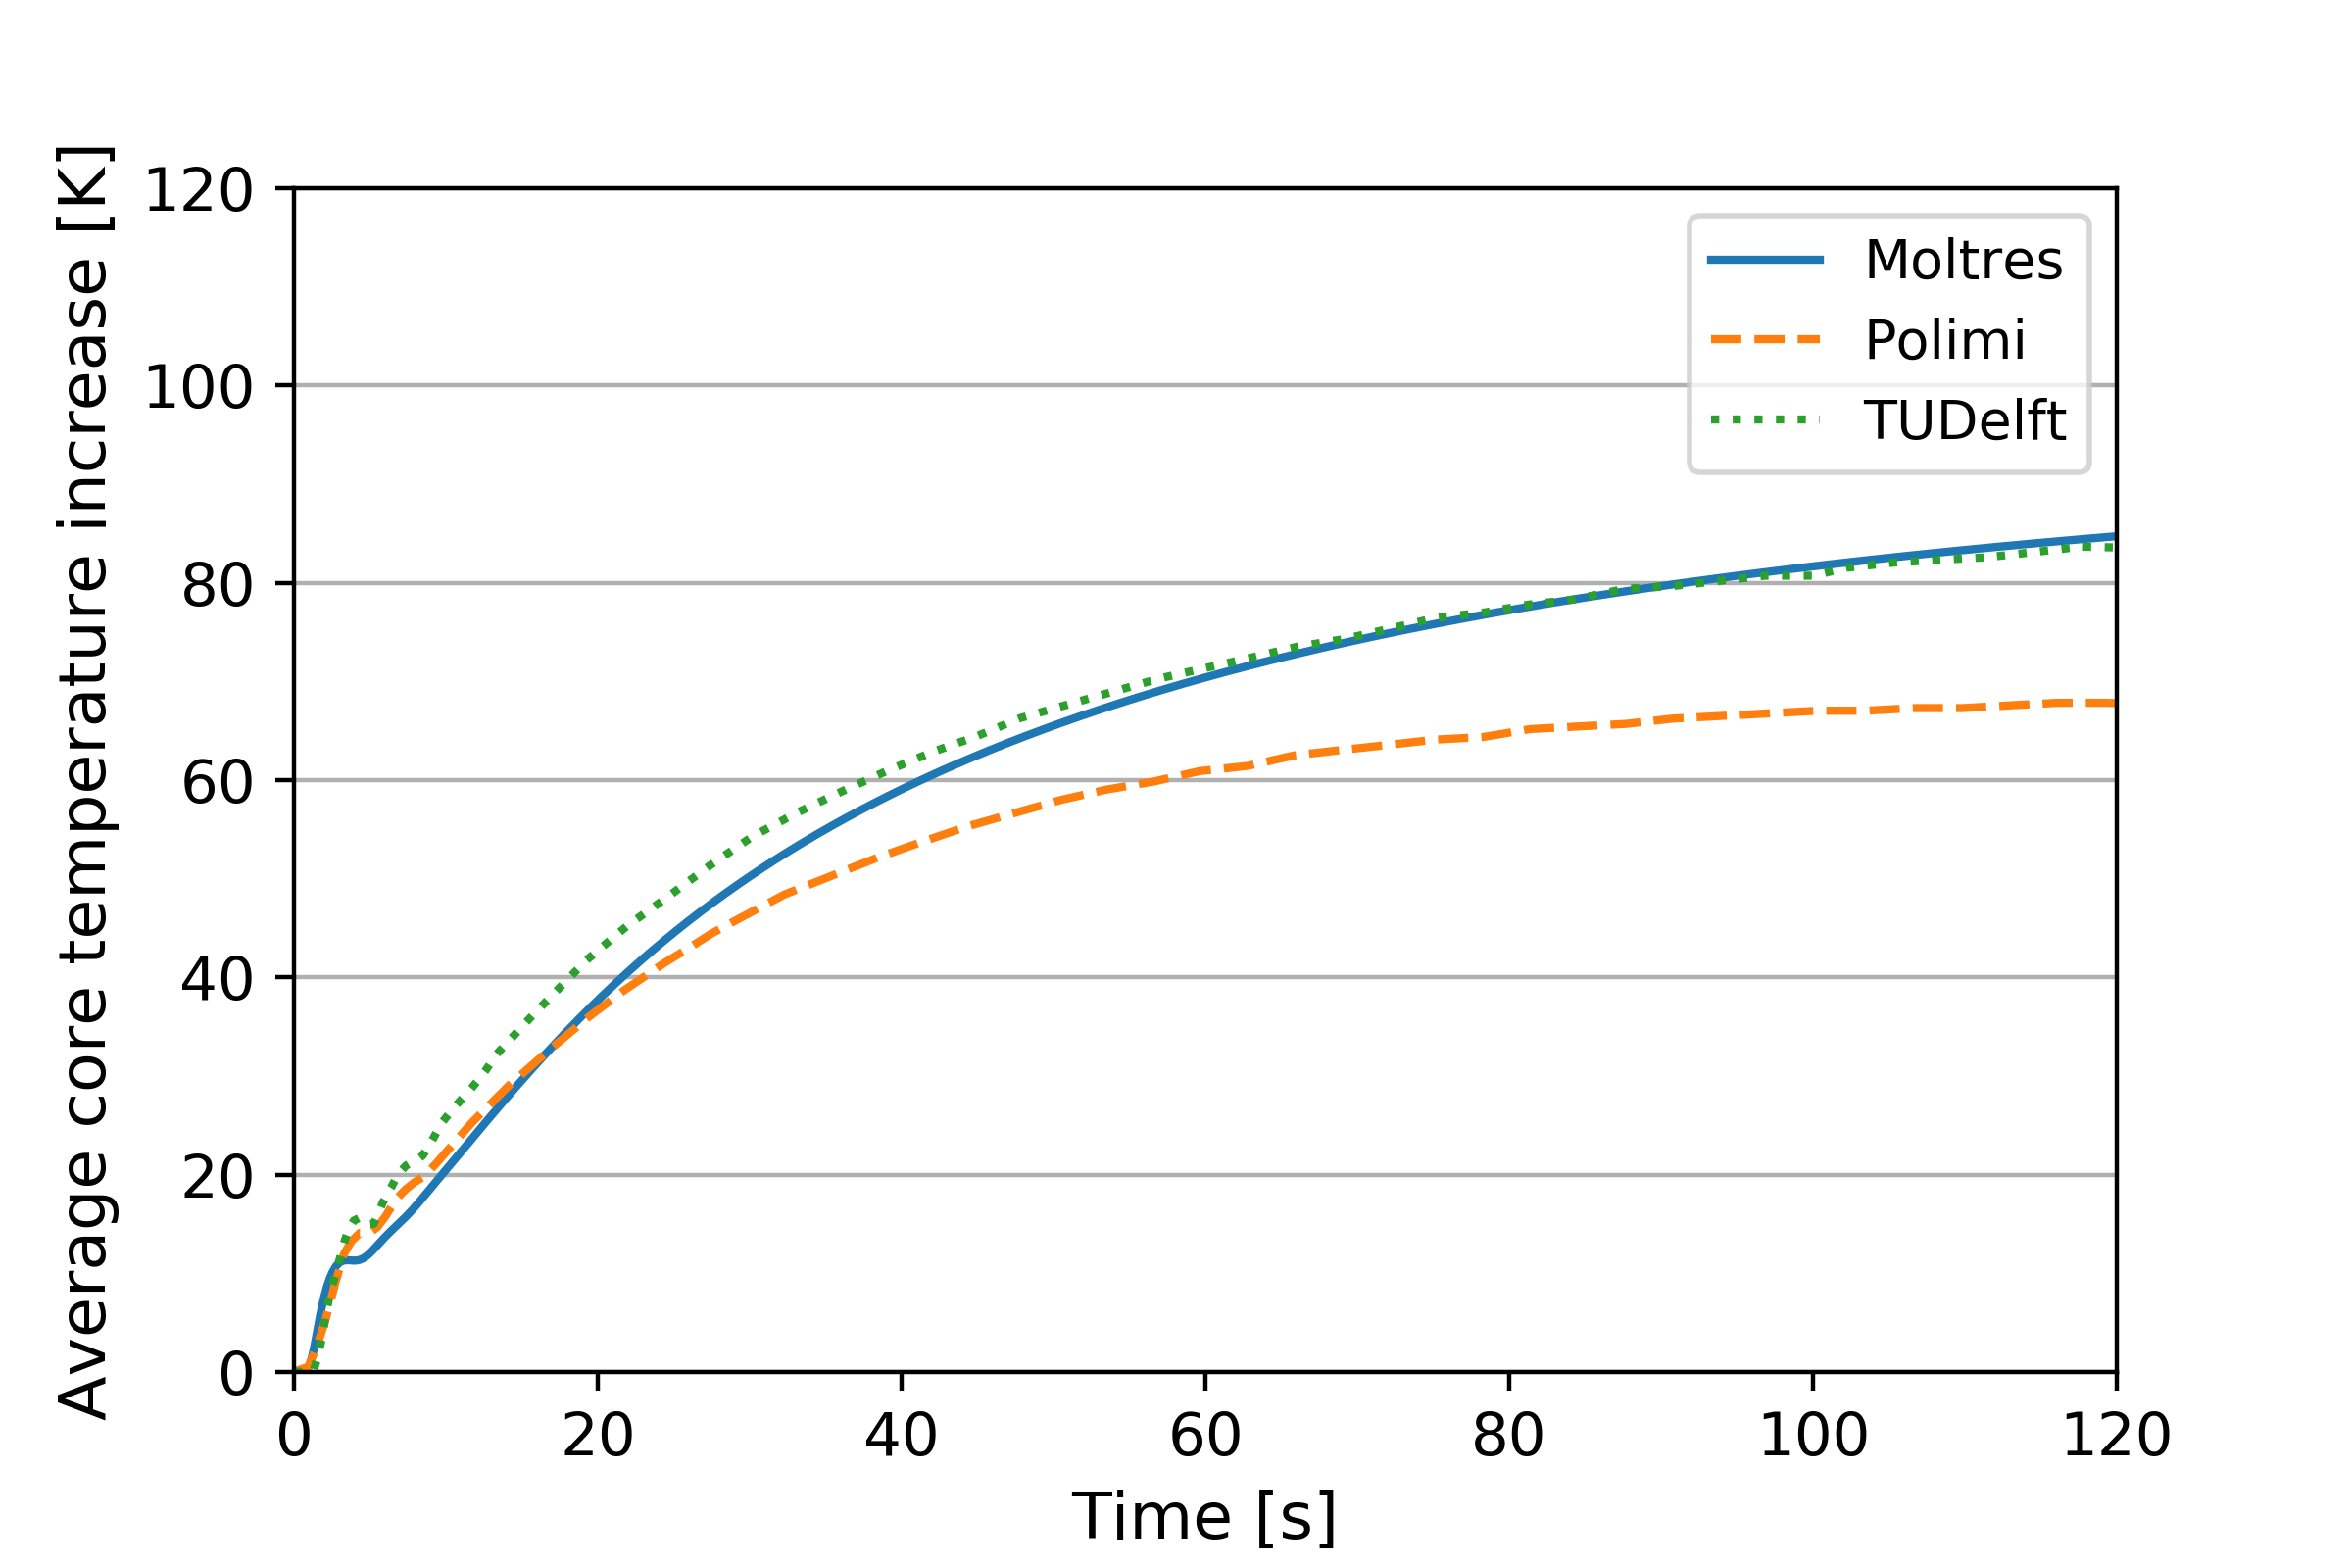
\includegraphics[width=.85\textwidth]{lohs-temp}
    \caption{Average core temperature increase during
    an unprotected loss of heat sink transient in the Moltres, Polimi, and
    TUDelft models \cite{fiorina_modelling_2014} without decay heat.}
    \label{fig:lohstemp}
\end{figure}

\clearpage

\subsection{With Decay Heat}

Decay heat from fission products poses a great safety risk in a loss of
heat sink accident. Section \ref{sec:wodecayheat} showed that prompt fission
power output quickly falls as core temperatures rise. However, decay power
output is independent of the instantaneous neutron flux. Figure
\ref{fig:moltresdecaypower} shows that the decay power output remains
relatively high during a short-term transient. Decay heat becomes the dominant
heat source from $t=34$ s and falls at a much slower rate than prompt heat.
Figure \ref{fig:moltresdecaytemp} highlights the
greater core temperature increase attributed to decay heat as compared with
the results without decay heat. By $t=120$ s, the model with decay heat
records an average core temperature increase that is 45 K higher than the
model without decay heat. The average core temperature reaches approximately
1220 K and would continue to rise further. This places undue thermal stress
and accelerate corrosion rates in the Hastelloy structural material. In the
absence of an auxiliary heat removal system in the primary loop, reactor
operators would have to rely on the freeze plug to drain the core into a drain
tank with emergency cooling systems to keep the salt cool.

\begin{figure}[htbp!]
    \centering
    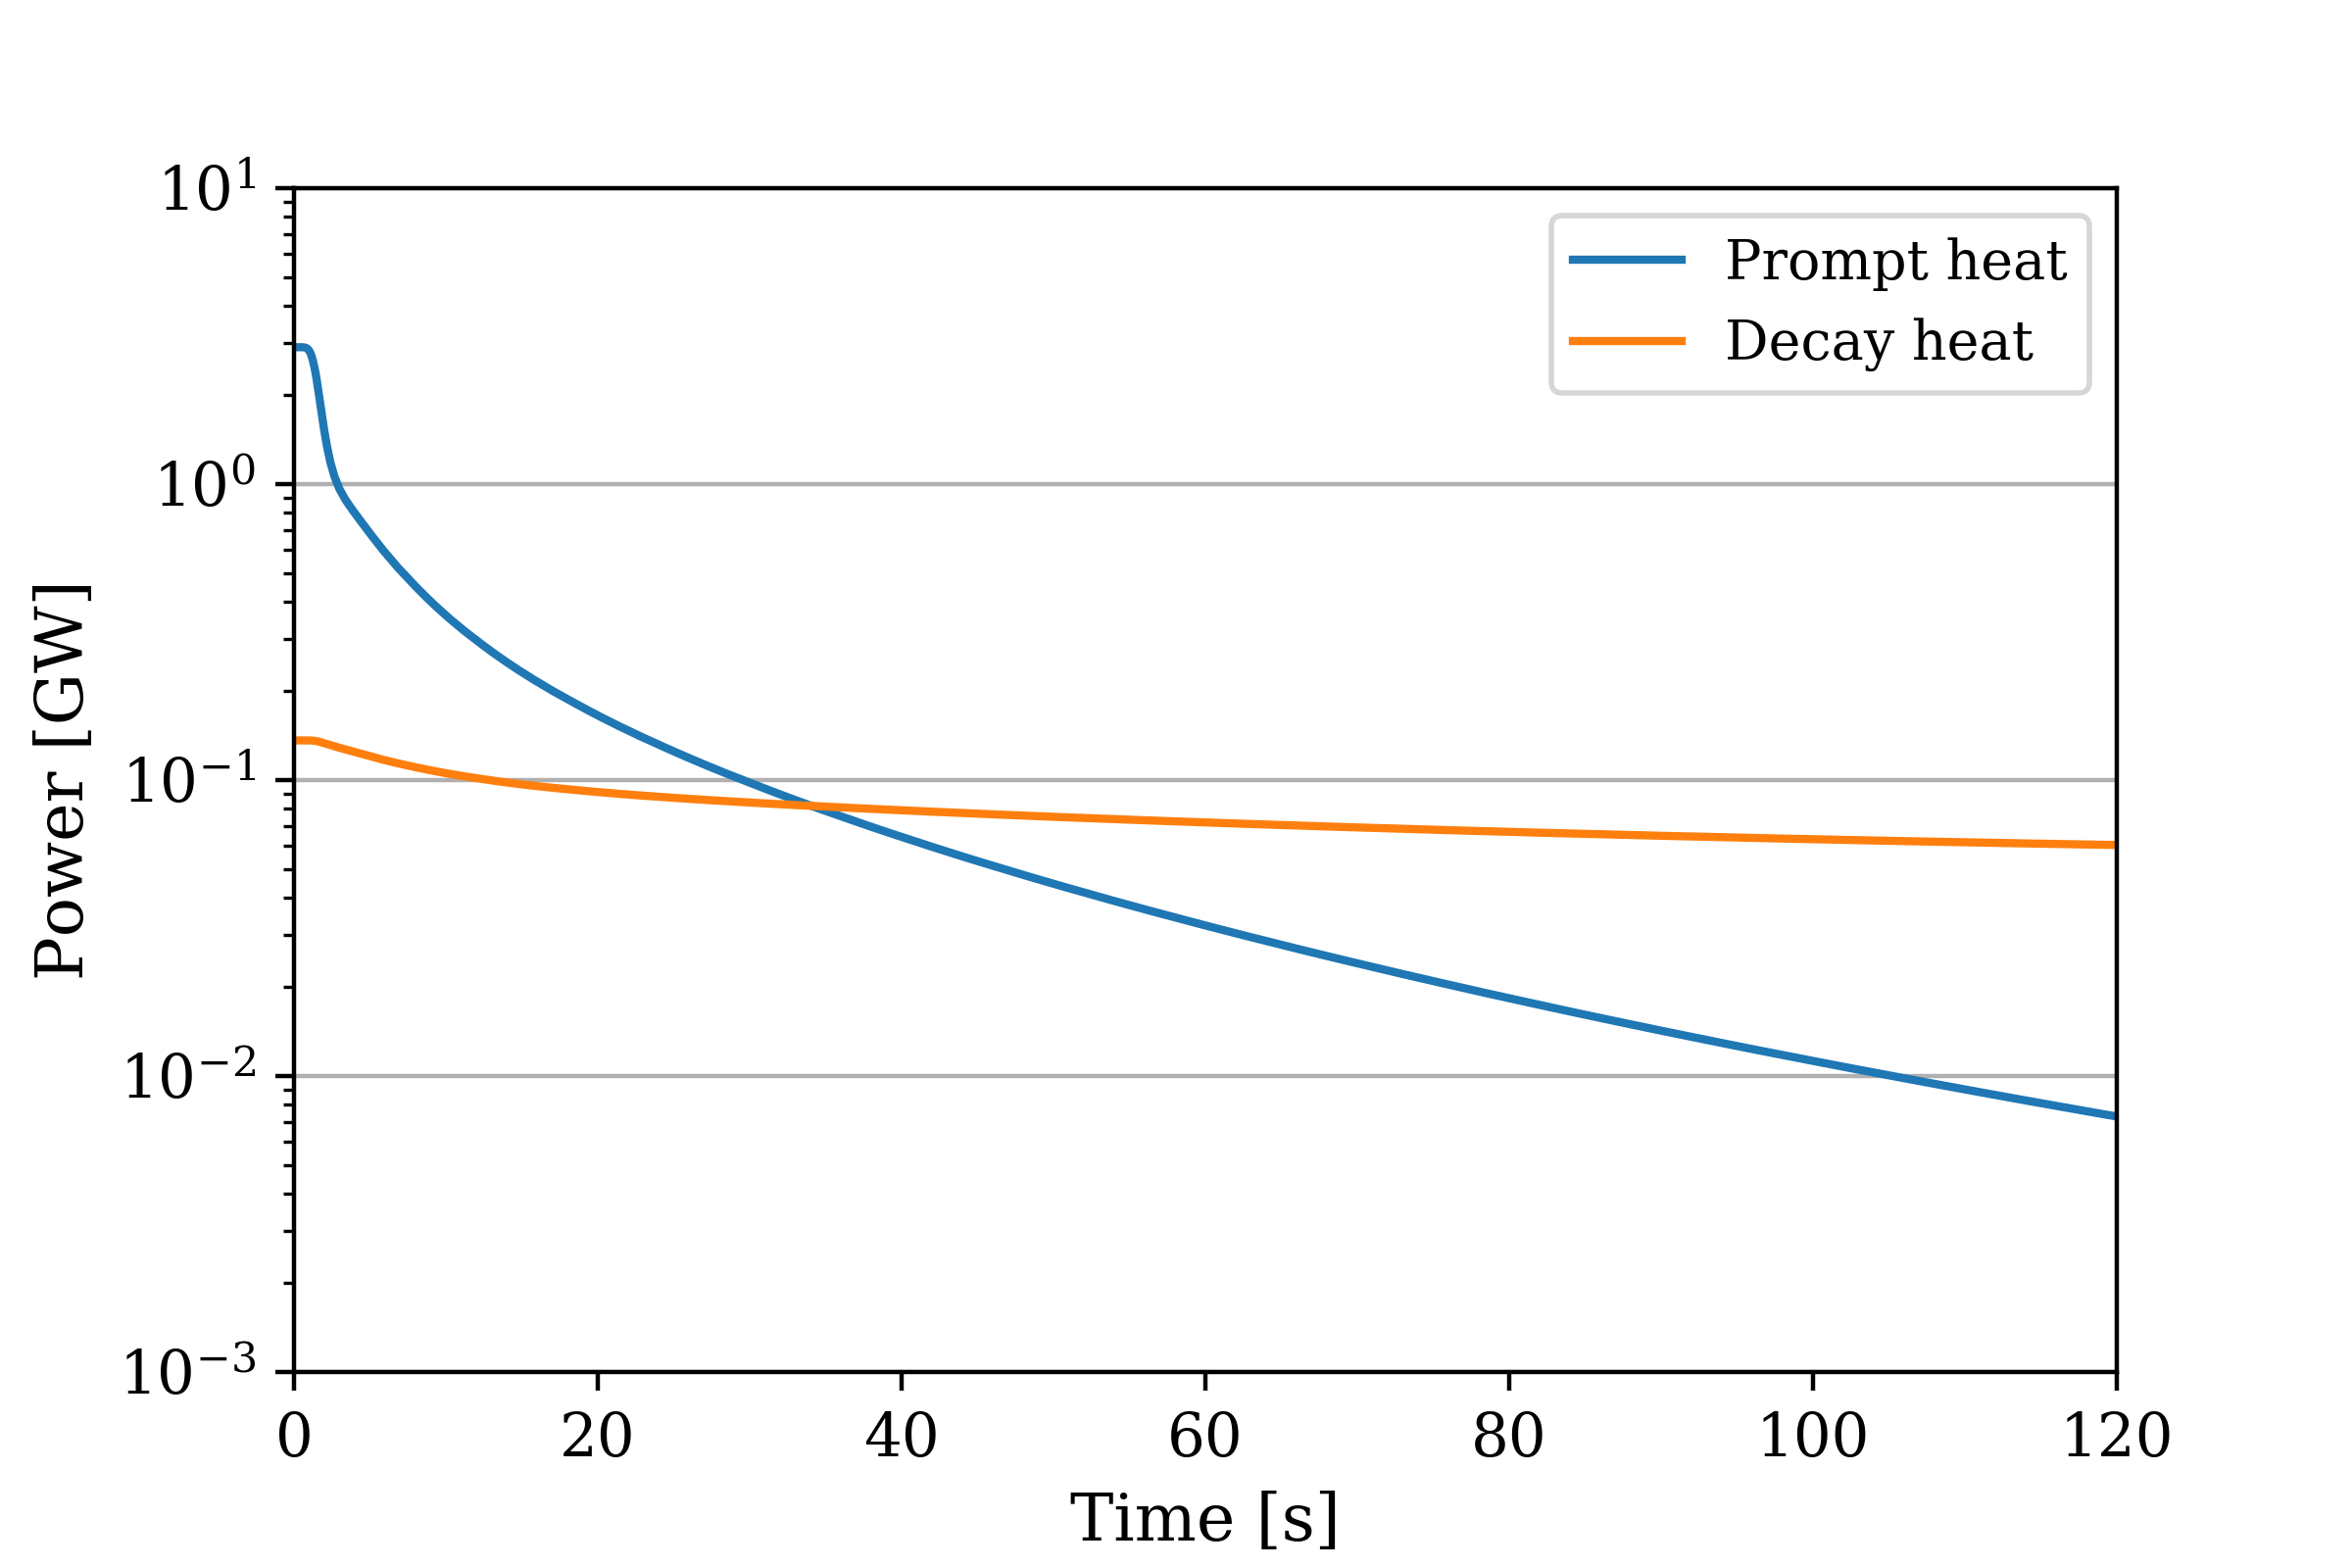
\includegraphics[width=.85\textwidth]{moltres-decay-power}
    \caption{Power output during
    an unprotected loss of heat sink transient in the Moltres model with and
    without decay heat.}
    \label{fig:moltresdecaypower}
    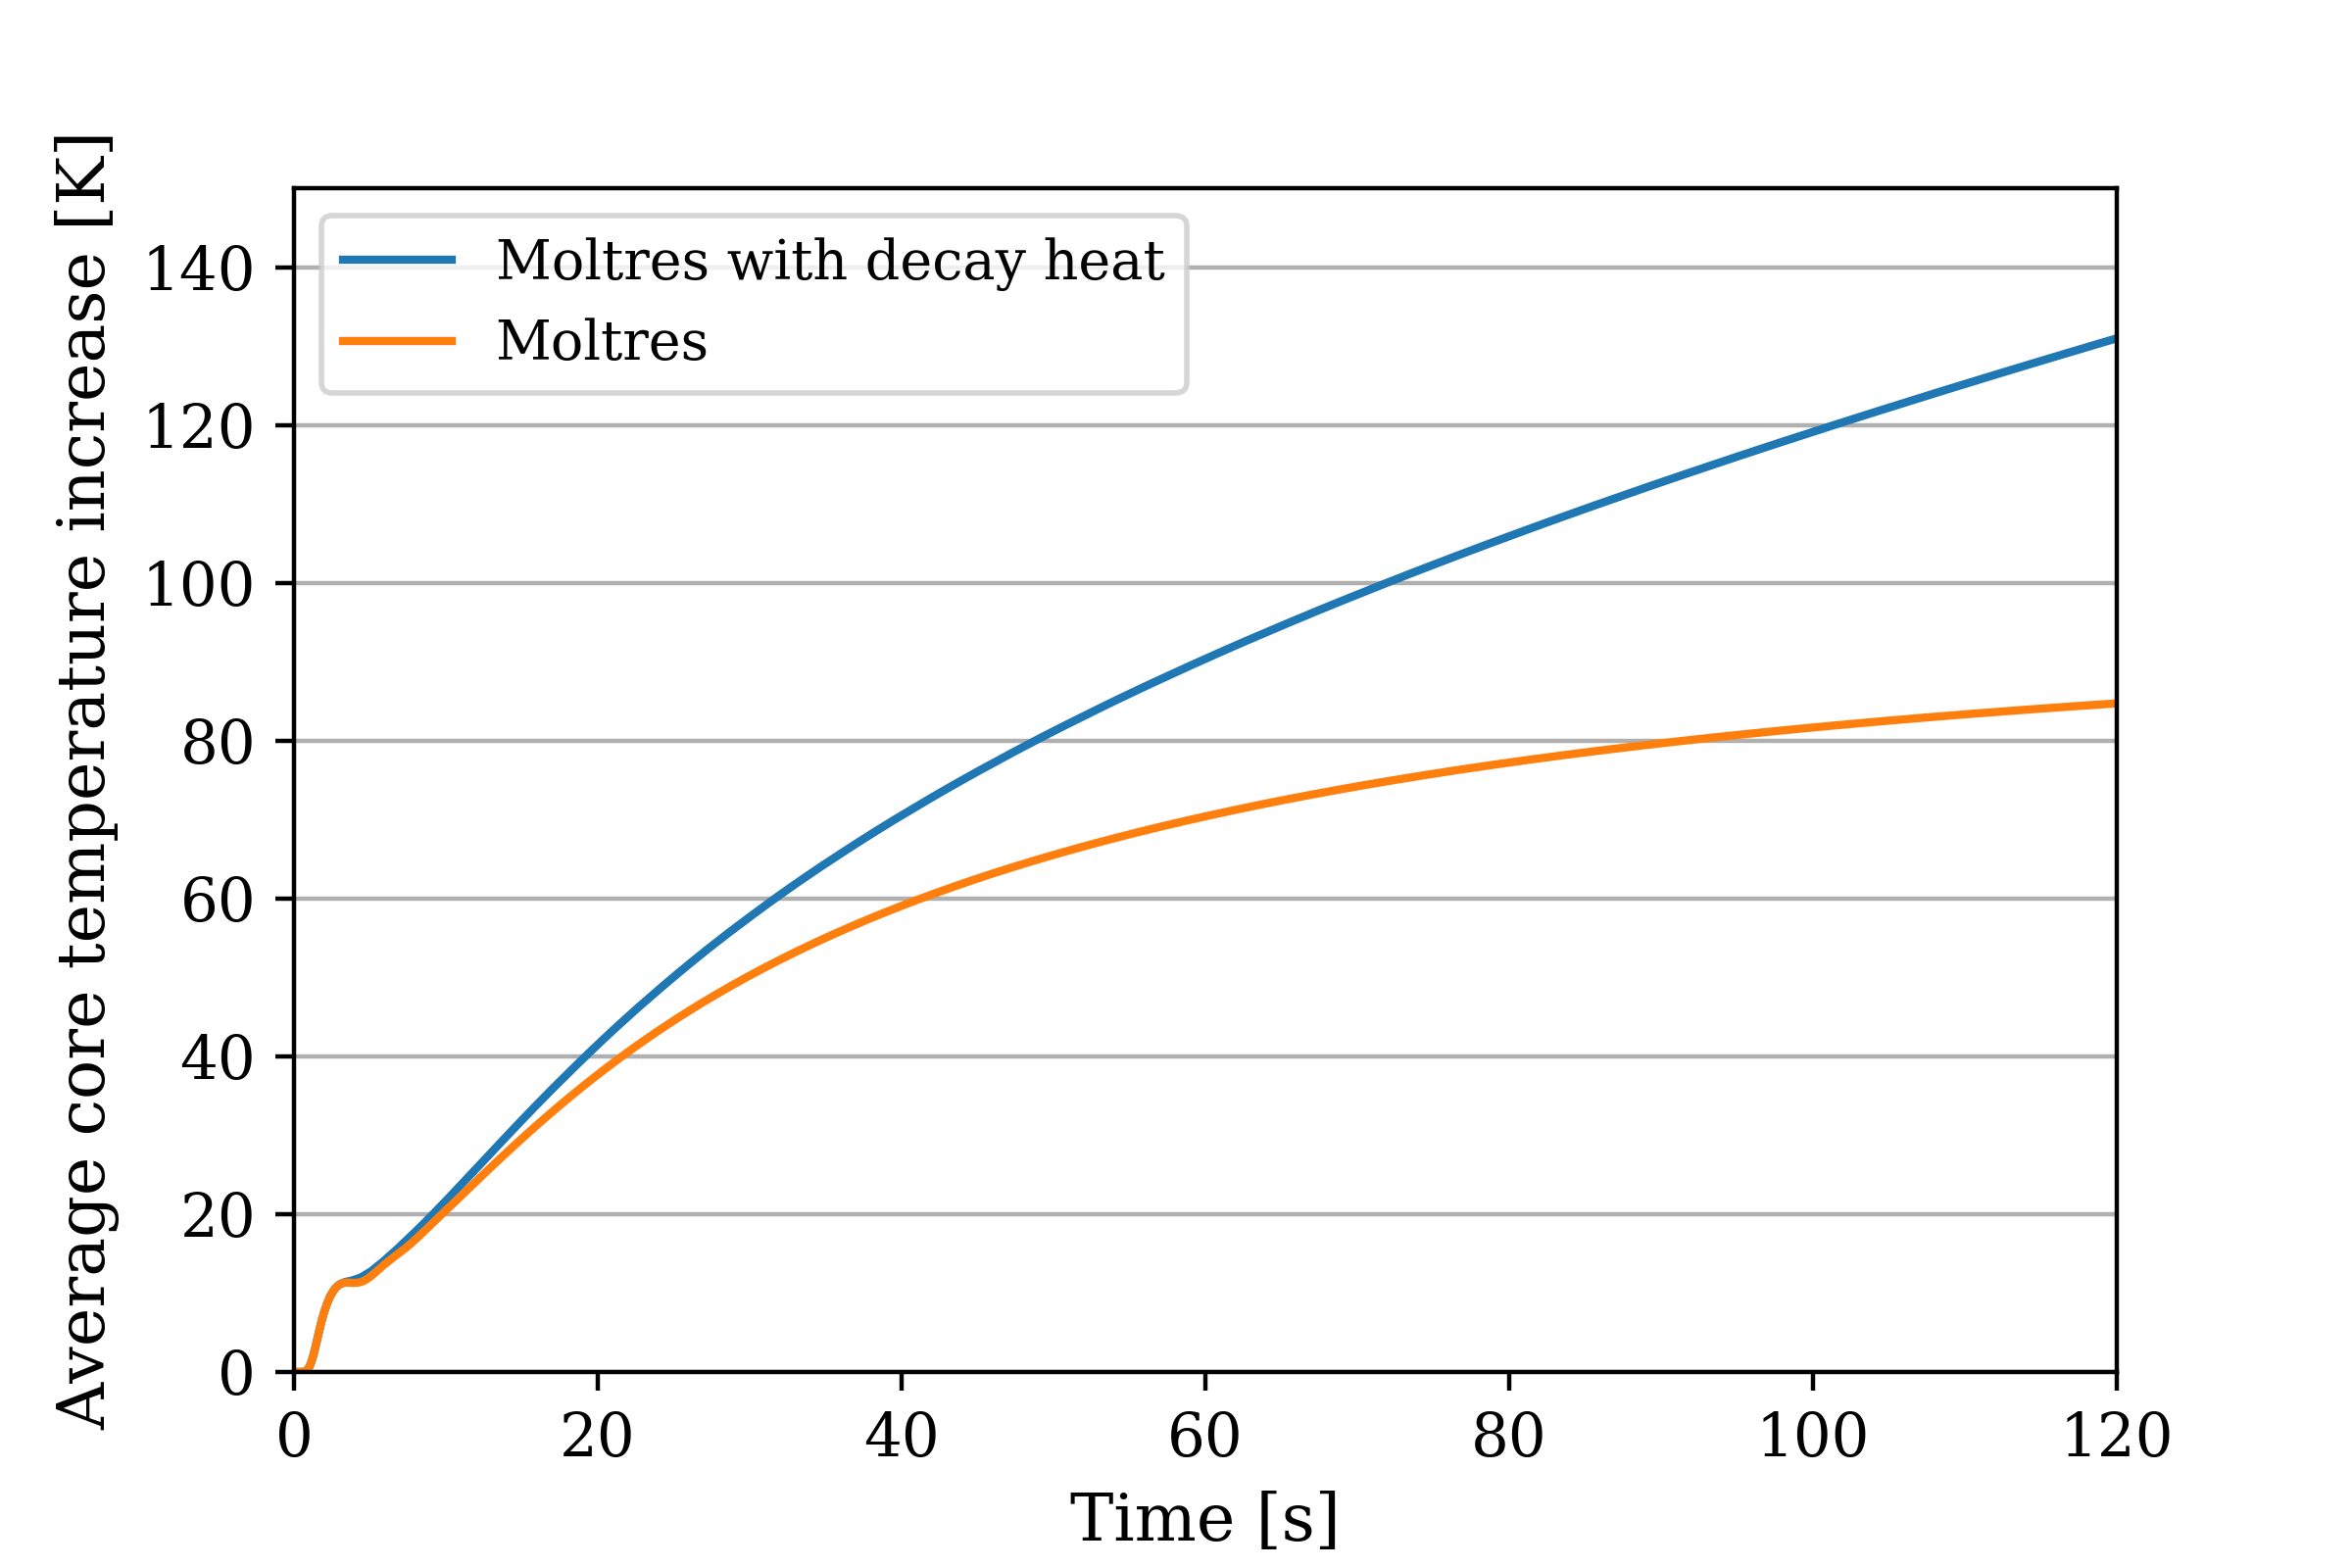
\includegraphics[width=.85\textwidth]{moltres-decay-temp}
    \caption{Average core temperature increase during
    an unprotected loss of heat sink transient in the Moltres model with and
    without decay heat.}
    \label{fig:moltresdecaytemp}
\end{figure}

\begin{figure}[htbp!]
    \centering
    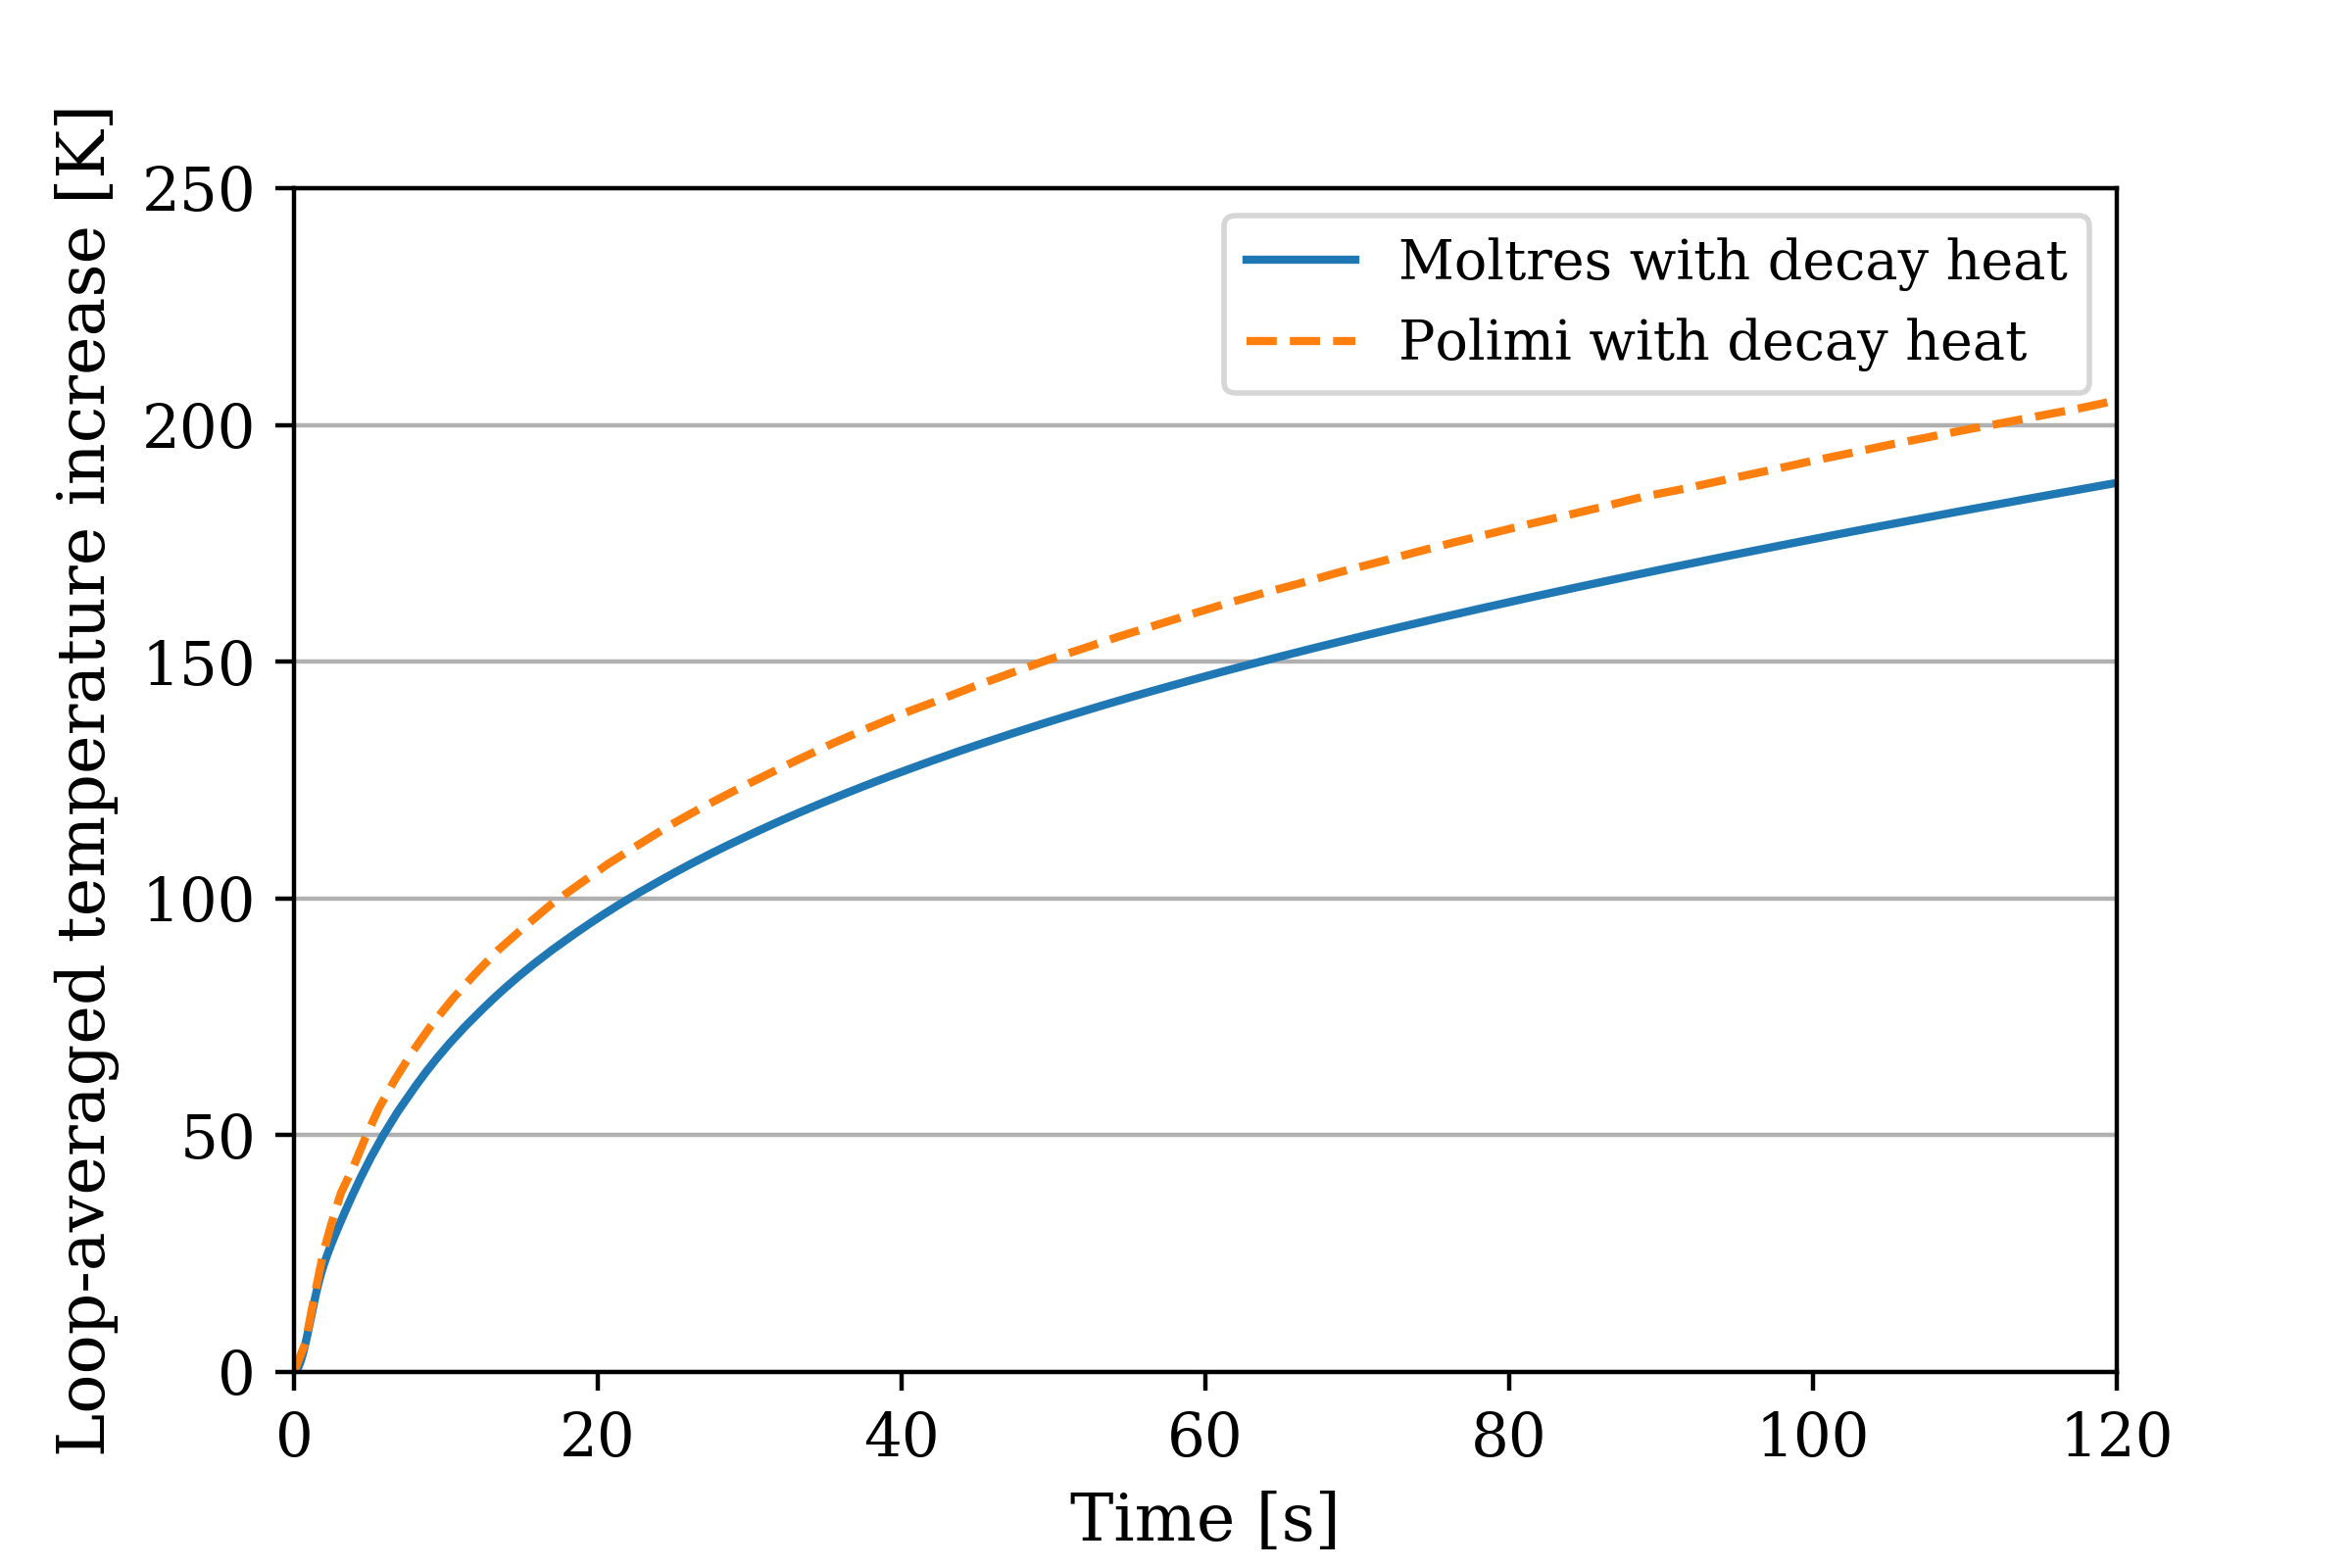
\includegraphics[width=.85\textwidth]{decay-temp}
    \caption{Loop-averaged temperature increase during
    an unprotected loss of heat sink transient in the Moltres and Polimi
    models \cite{fiorina_modelling_2014} with decay heat.}
    \label{fig:polimidecaytemp}
\end{figure}

Figure \ref{fig:polimidecaytemp} shows the loop-averaged temperature
increase in the Moltres and Polimi models \cite{fiorina_modelling_2014}. The
TUDelft model does not have a decay heat modeling capability. The Moltres
model predicts the same increasing trend in the temperature. The loop-averaged
temperature rises significantly at the start of the transient and continues to
rise at a decreasing rate. The loop-averaged temperature increase in the
Moltres model at $t=120$ s is approximately 17 K lower than that in the Polimi
model. It is difficult to ascertain the exact cause for this difference
without the power profile from the Polimi model with decay heat to compare
with. However, if the decay power output are similar, the stronger negative
temperature reactivity coefficient would cause the prompt power output in the
Moltres model to fall faster than the Polimi model. Consequently, the
loop-averaged temperature would be lower as shown in the figure. Overall, the
results for the loss of heat sink transient agree with the Polimi and TUDelft
model results in both cases, with and without decay heat modeling.

\clearpage

\section{Unprotected Loss of Flow}

A loss of forced flow transient can occur in the event of a station
blackout; the pumps would cease operating due to the loss of AC electrical
power. Natural circulation resulting from temperature-dependent density
changes becomes the dominant driving force for salt flow in the primary loop.
Fiorina et al. \cite{fiorina_modelling_2014} applied the Boussinesq
approximation for buoyancy-driven flow in their models, but this approach was
not possible in Moltres because the primary loop is partitioned into two
separate geometries and used Dirichlet boundary
conditions at the inlet to drive flow. Fiorina et al.'s Polimi and TUDelft
models featured complete exponential coast-downs of the pumps with a time
constant of 5 s. The resulting flow rate $\dot{m}$ from natural circulation
was approximately 18 times smaller than the initial $\dot{m}$. Figure
\ref{fig:flowrate} shows that the actual $\dot{m}$ decreased with a time
constant of 8 s. Thus, for the \gls{MSFR} model in Moltres, this work imposed
a similar exponential decay term with a time constant of 8 s on the inflow
Dirichlet boundary condition:
%
\begin{align}
    \text{Flow rate, } v = 0.25862 + (4.5-0.25862) e^{-t/8} 
    \label{eq:flowrate}
\end{align}

\begin{figure}[htbp!]
    \centering
    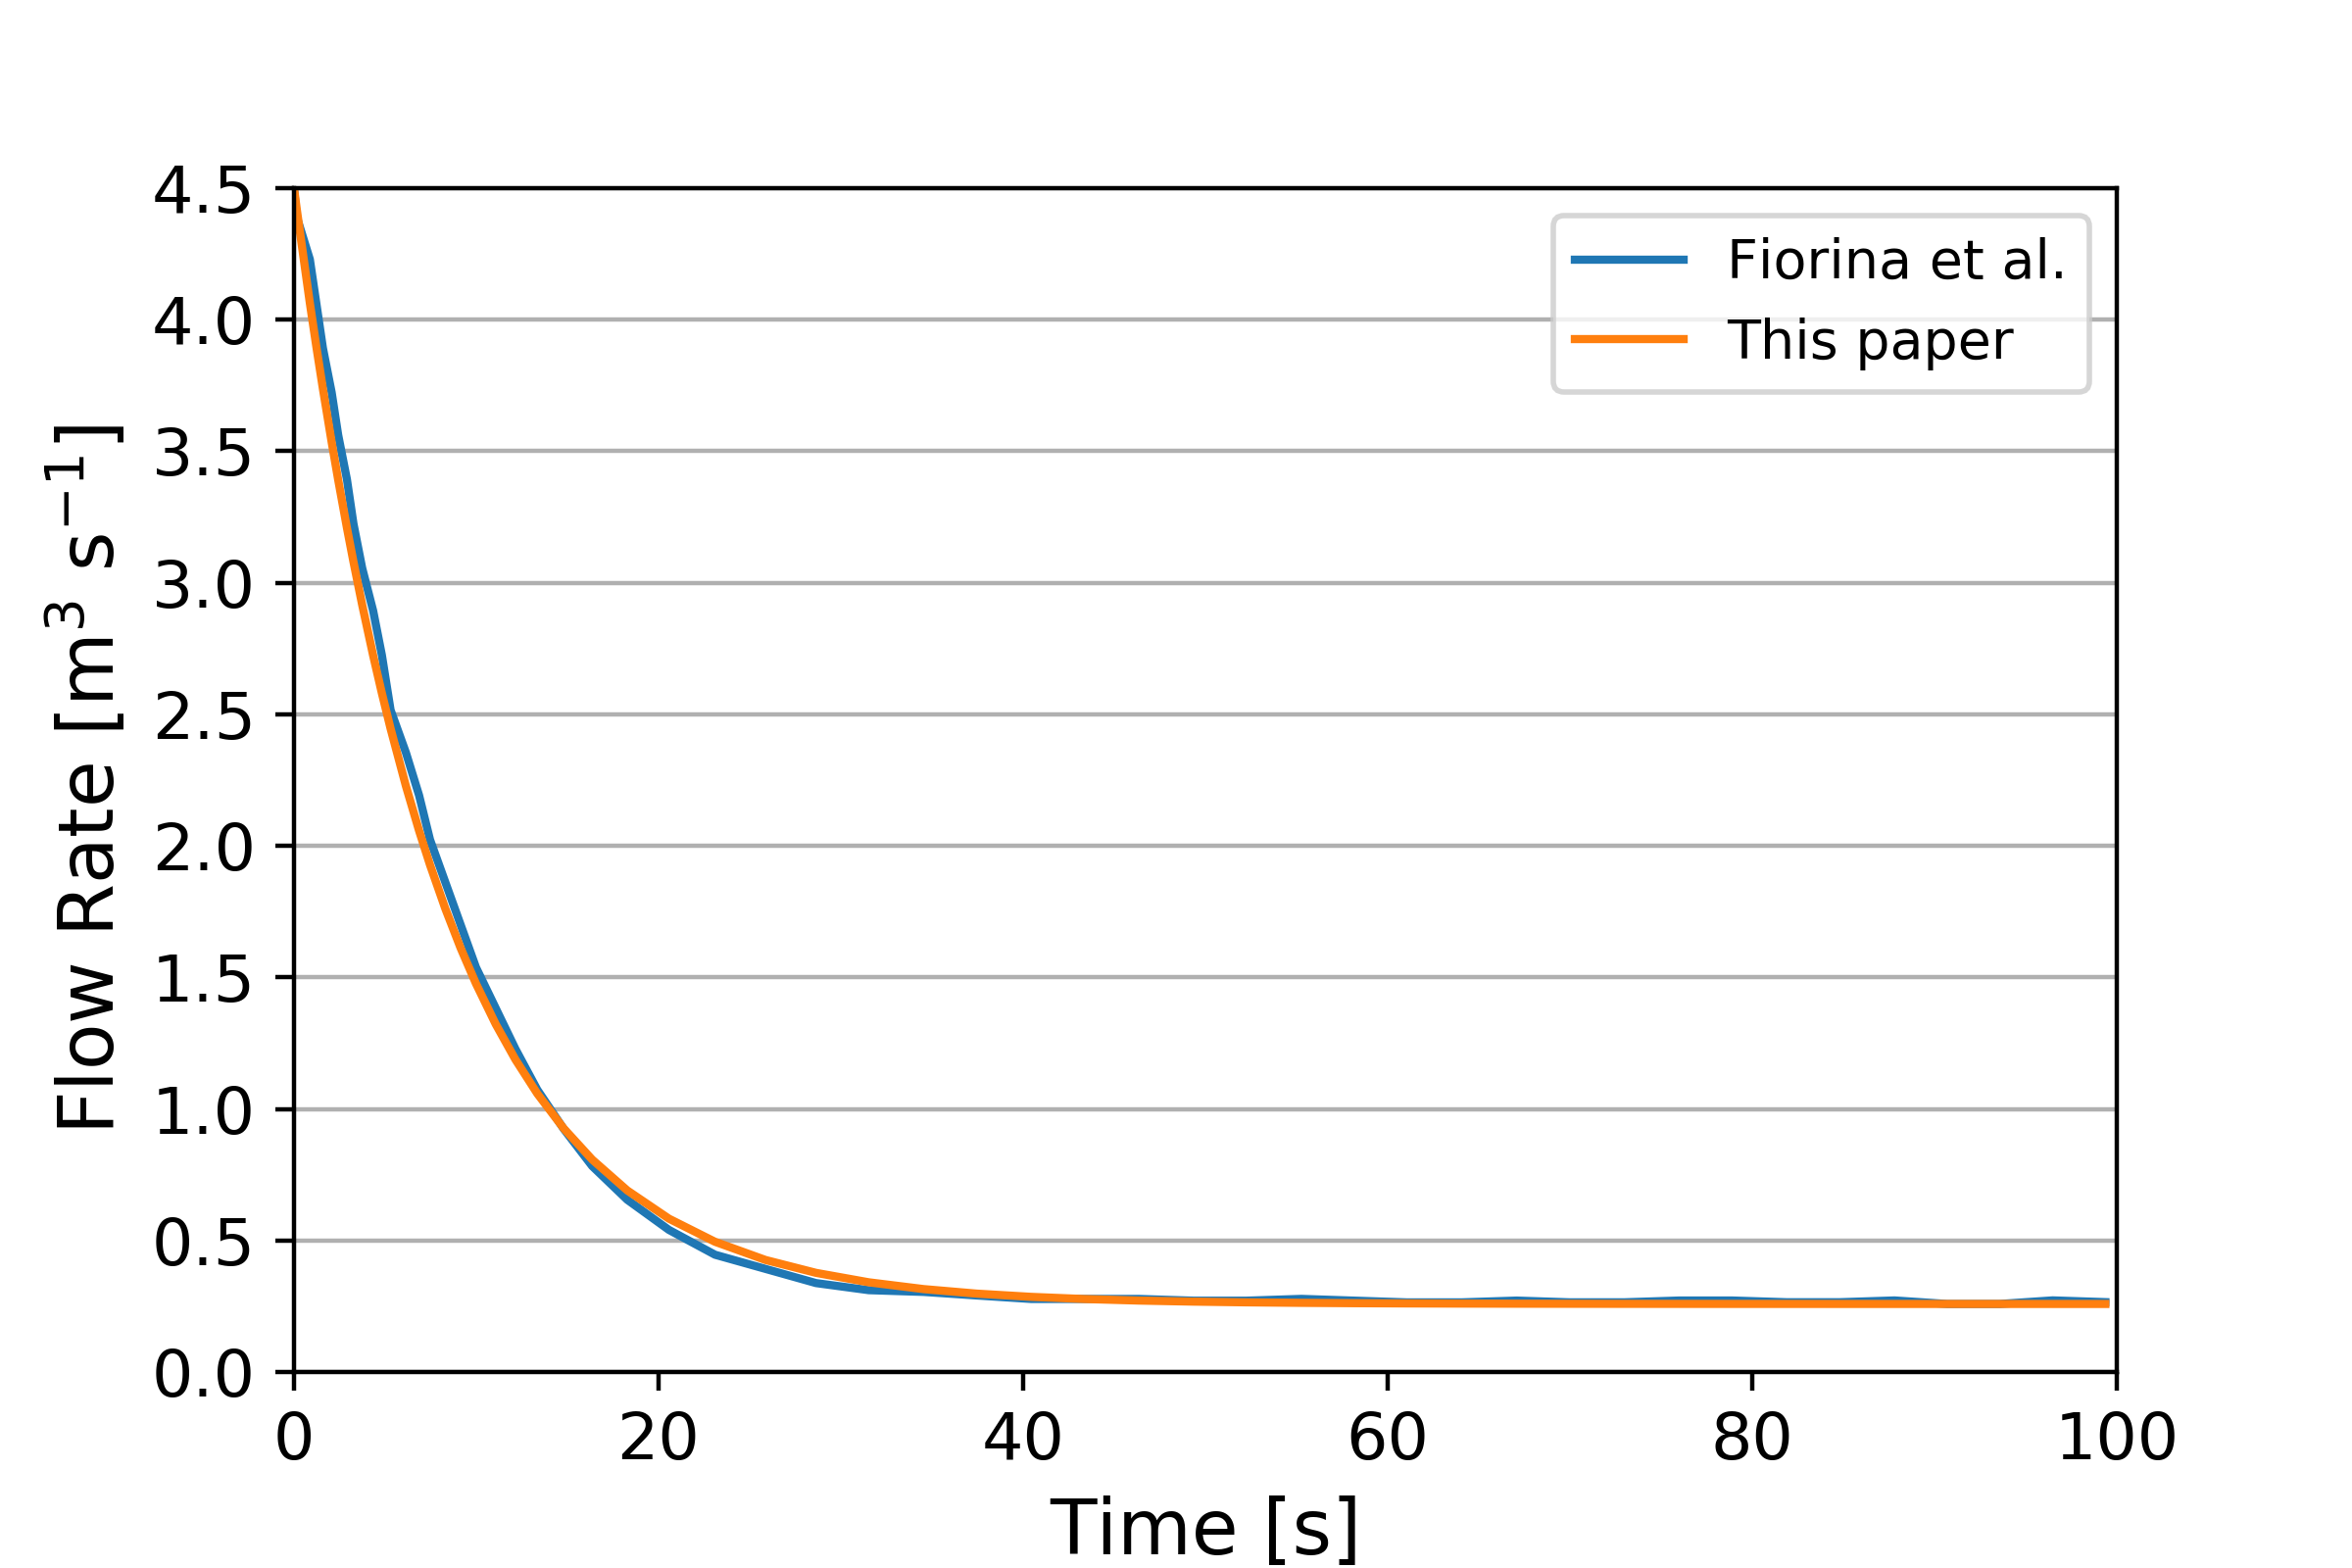
\includegraphics[width=.7\textwidth]{lof-flow-rate}
    \caption{The change in flow rate in the Polimi and TUDelft models and the
    imposed flow rate in Moltres.}
    \label{fig:flowrate}
\end{figure}

The reduced $\dot{m}$ also decreases the heat transfer rate between the
primary and intermediate loop through the heat exchanger as the heat transfer
coefficient $h$ is dependent on the $\dot{m}$. This step was problematic
because
the pointwise heat exchanger implementation in Moltres performs differently
compared with the heat exchangers that take up ``36\% of the out-of-core
part'' in the Polimi and TUDelft models \cite{fiorina_modelling_2014}. Most of
the cooling happens in the top half of the heat exchanger where the
temperature differential between the primary and intermediate loops is the
largest. In the Polimi and TUDelft models, the overall $h$ is the
``harmonic mean of the heat transfer coefficients on each side of the heat
exchanger''. For this loss of flow transient, the authors intended to focus on
the primary loop and assumed that only the pumps in the primary loop failed.
In addition to this, the authors applied the Dittus-Boelter correlation
\cite{dittus_heat_1930} for the relationship between the primary side $h$ and
$\dot{m}$. The Dittus-Boelter correlation for fluids being cooled is:
%
\begin{align}
    Nu &= 0.023 Re^{0.8} Pr^{0.3} \label{eq:db} \\
    \intertext{where}
    Nu &= \text{ Nusselt number,} \nonumber \\
    Re &= \text{ Reynolds number,} \nonumber \\
    Pr &= \text{ Prandtl number.} \nonumber
\end{align}
%
The only direct relation to $\dot{m}$ in the Dittus-Boelter correlation is
through the $Re$ term, which is directly proportional to flow velocity $v$.
This gives the following relation between $h$ and$v$:
%
\begin{align}
    h \propto v^{0.8} \label{eq:hv}
\end{align}
%
However, this relation provided very different results in the unprotected loss
of flow and pump overspeed transients compared with the Polimi and TUDelft
models; it overpredicted the equilibrium power output in the
unprotected loss of flow transient and underpredicted the same parameter in
the unprotected pump overspeed transient. Upon further investigation, the
present author found that raising the power of $v$ from 0.8 to 1.1 brought the
average core temperatures closer to the results from the other models in both
transients. Therefore, this work adopted the raised power in this study.

Another issue pertained to the turbulent viscosity $\mu_t$ as a function of
$v$. Using a simple approximation of $\mu_t$ being directly
proportional to $v$, the results differed significantly compared with the
Polimi and TUDelft models. This is likely due to buoyancy-driven flow
contributing to turbulence; the turbulent energy $k$ equation in COMSOL's
$k$-$\epsilon$ model has an explicit source term from buoyancy effects
\cite{comsol_ab_comsol_2018}. Another point to note is the
Reynolds number remains constant if $\mu$ and $v$ decrease in tandem. This
preserves the existence of the recirculation zone in the core and it is at
odds with the results from the Polimi and TUDelft models, which show that the
recirculation zones disappear during the loss of flow transient. We
circumvented this issue by letting fixed fractions of the initial $\mu_{t,0}$
be conserved regardless of the final flow velocity, according to the following
equation:
%
\begin{align}
    \mu_t &= \mu_c + (\mu_{t,0} - \mu_c) e^{-t/8} \label{lofmu} \\
    \intertext{where}
    \mu_c &= \text{ conserved fraction of $\mu_{t,0}$ [Pa$\cdot$s].} \nonumber
\end{align}
%
This measure allowed for laminar flow to develop in the core and yielded
results with closer resemblance to those from the Polimi and TUDelft models.

Figures \ref{fig:lofheat} and \ref{fig:loftemp} show the power output and
average core temperature increase during the unprotected loss of flow
transient in the Moltres, Polimi, and TUDelft models without decay heat
modeling. The three sets of results from Moltres correspond to $\mu_c =
\frac{1}{4} \mu_{t,0}, \frac{1}{2} \mu_{t,0}, \text{and } \frac{3}{4}
\mu_{t,0}$. Moltres
performs poorer in this transient relative to the two previous transients.
Although Moltres shows the same decreasing trend in power output, it failed to
capture the exact individual features in the reactor response. In the Polimi 
and TUDelft models, Fiorina et al.
stated that after around $t=15$ s, the ``flow pattern changed in the core and
the recirculation zones started to disappear''. A sudden drop in the average
core temperature results as the pocket of hot salt leaves the
core. In Moltres, the wider peak in the average core temperature
indicates that there was a more gradual change in the flow pattern.

\begin{figure}[htbp!]
    \centering
    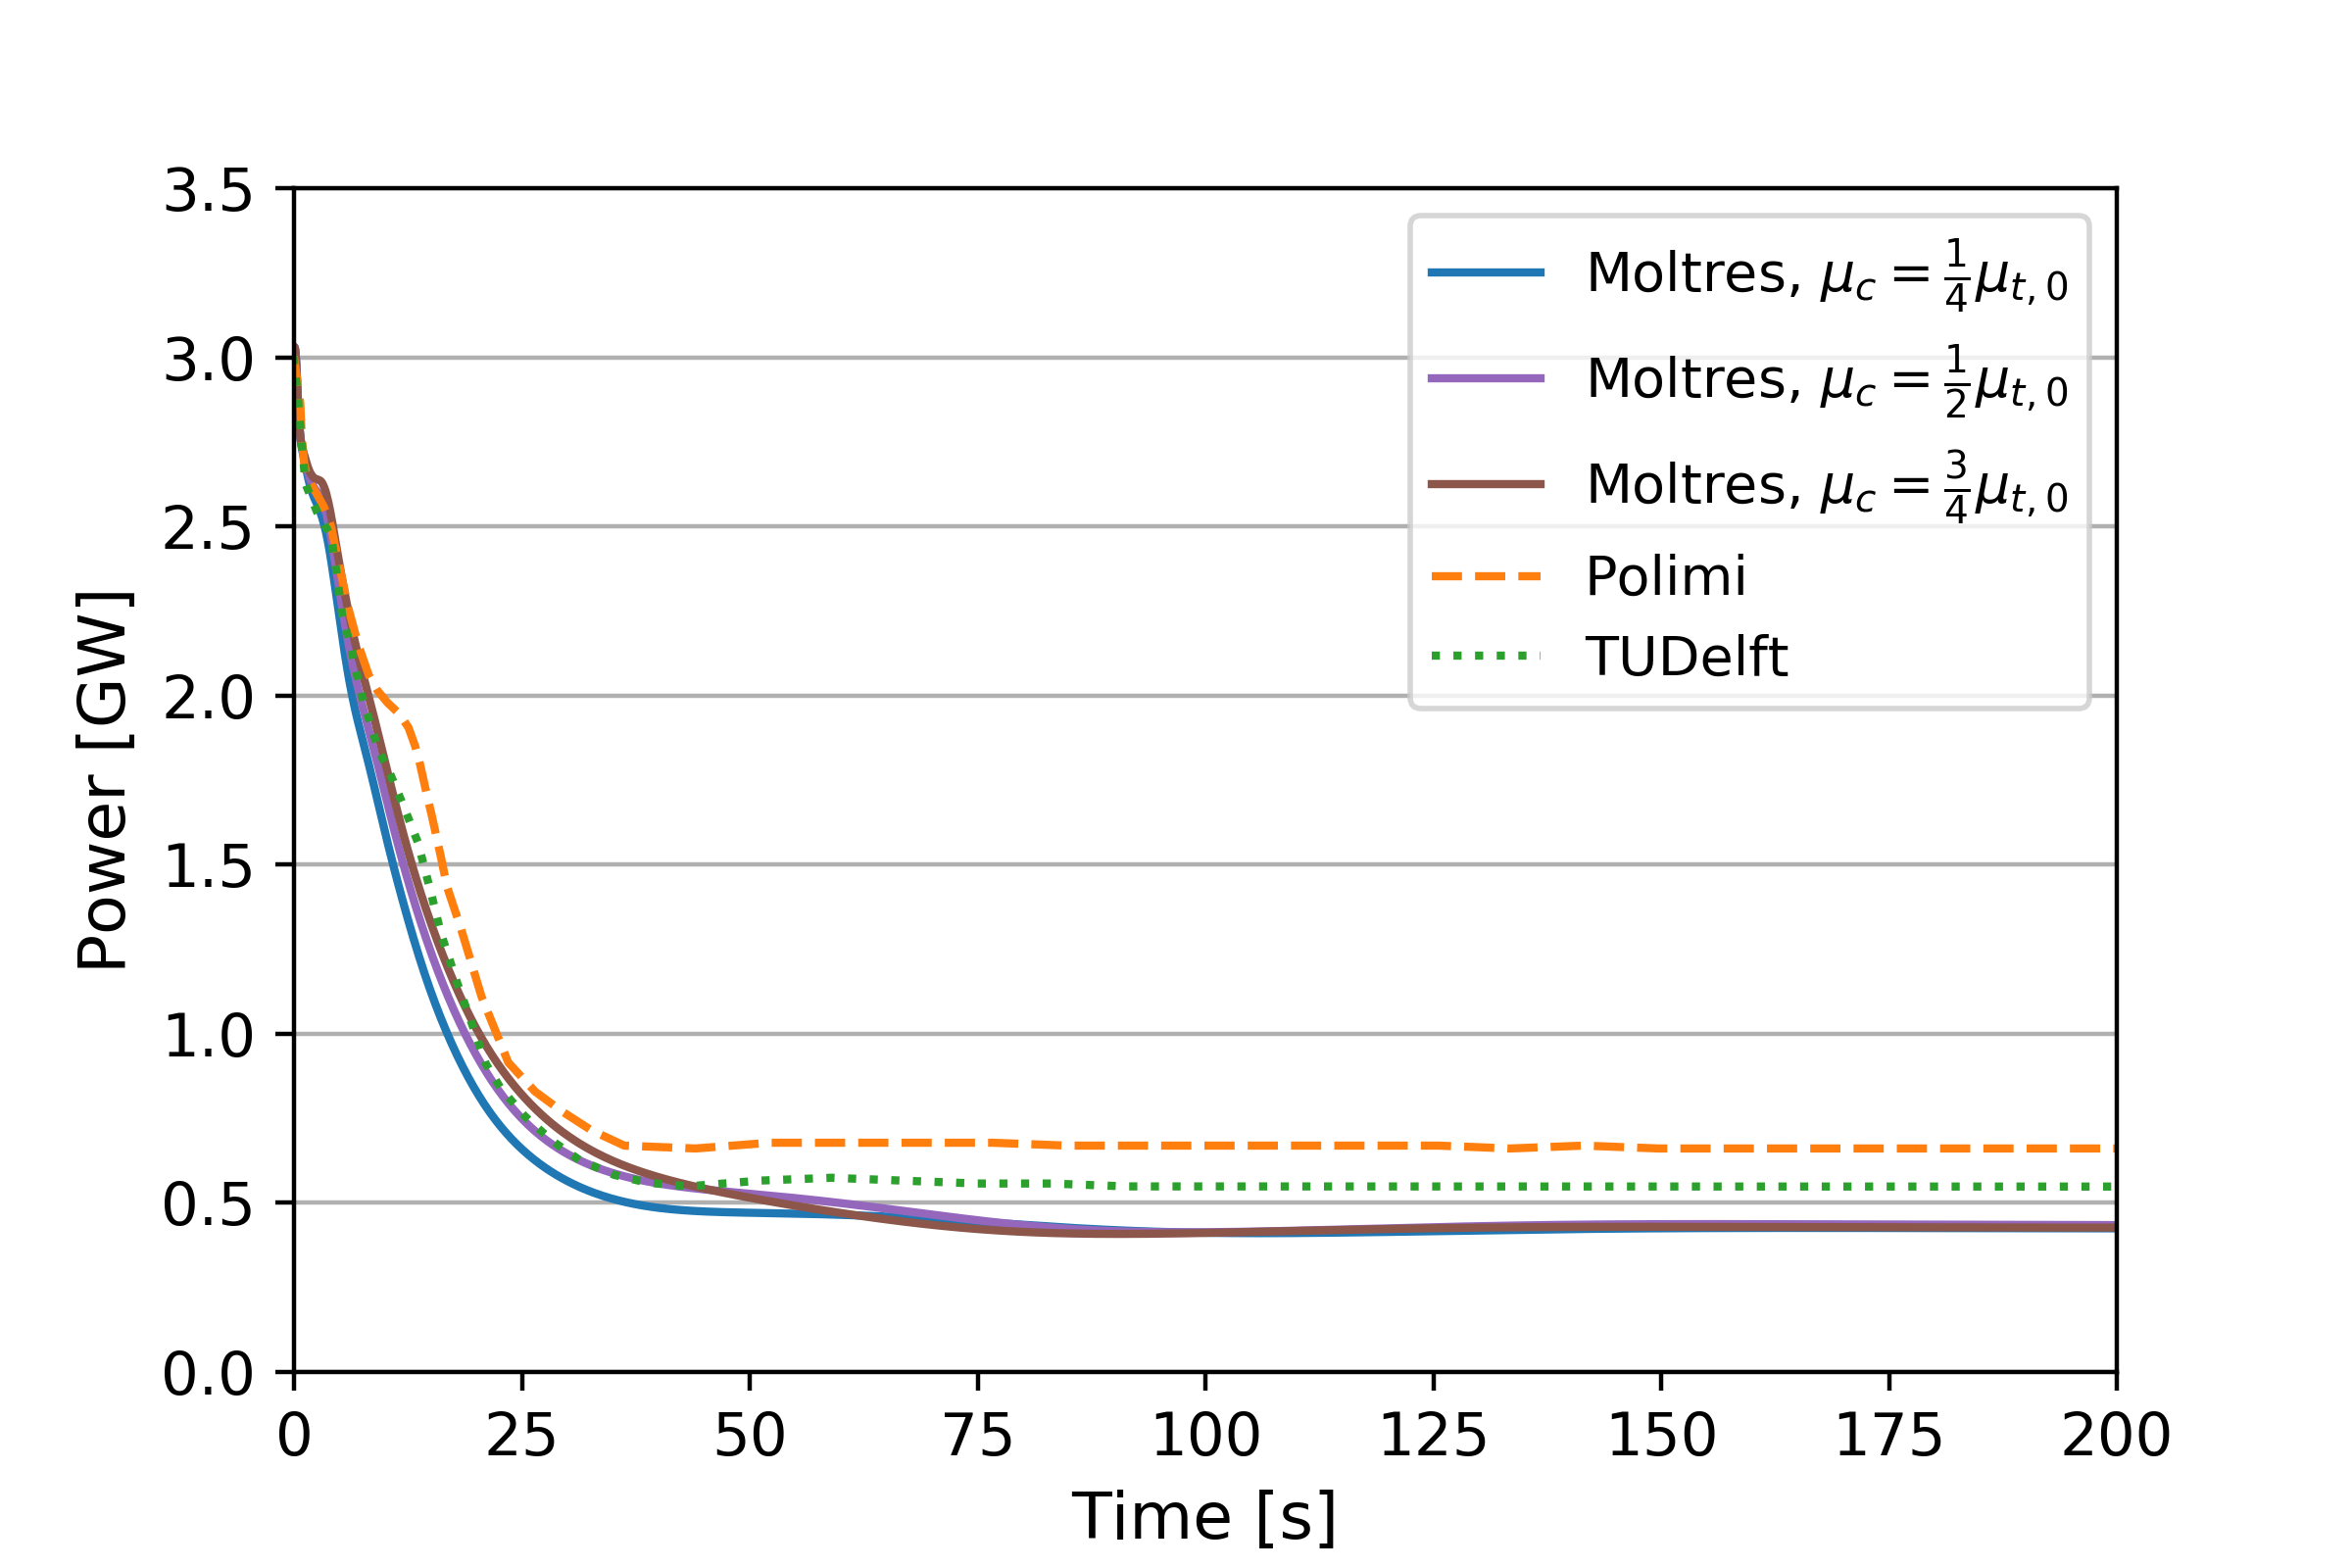
\includegraphics[width=.85\textwidth]{lof-heat}
    \caption{Power output during
    an unprotected loss of flow transient in the Moltres, Polimi, and
    TUDelft models \cite{fiorina_modelling_2014}.}
    \label{fig:lofheat}
    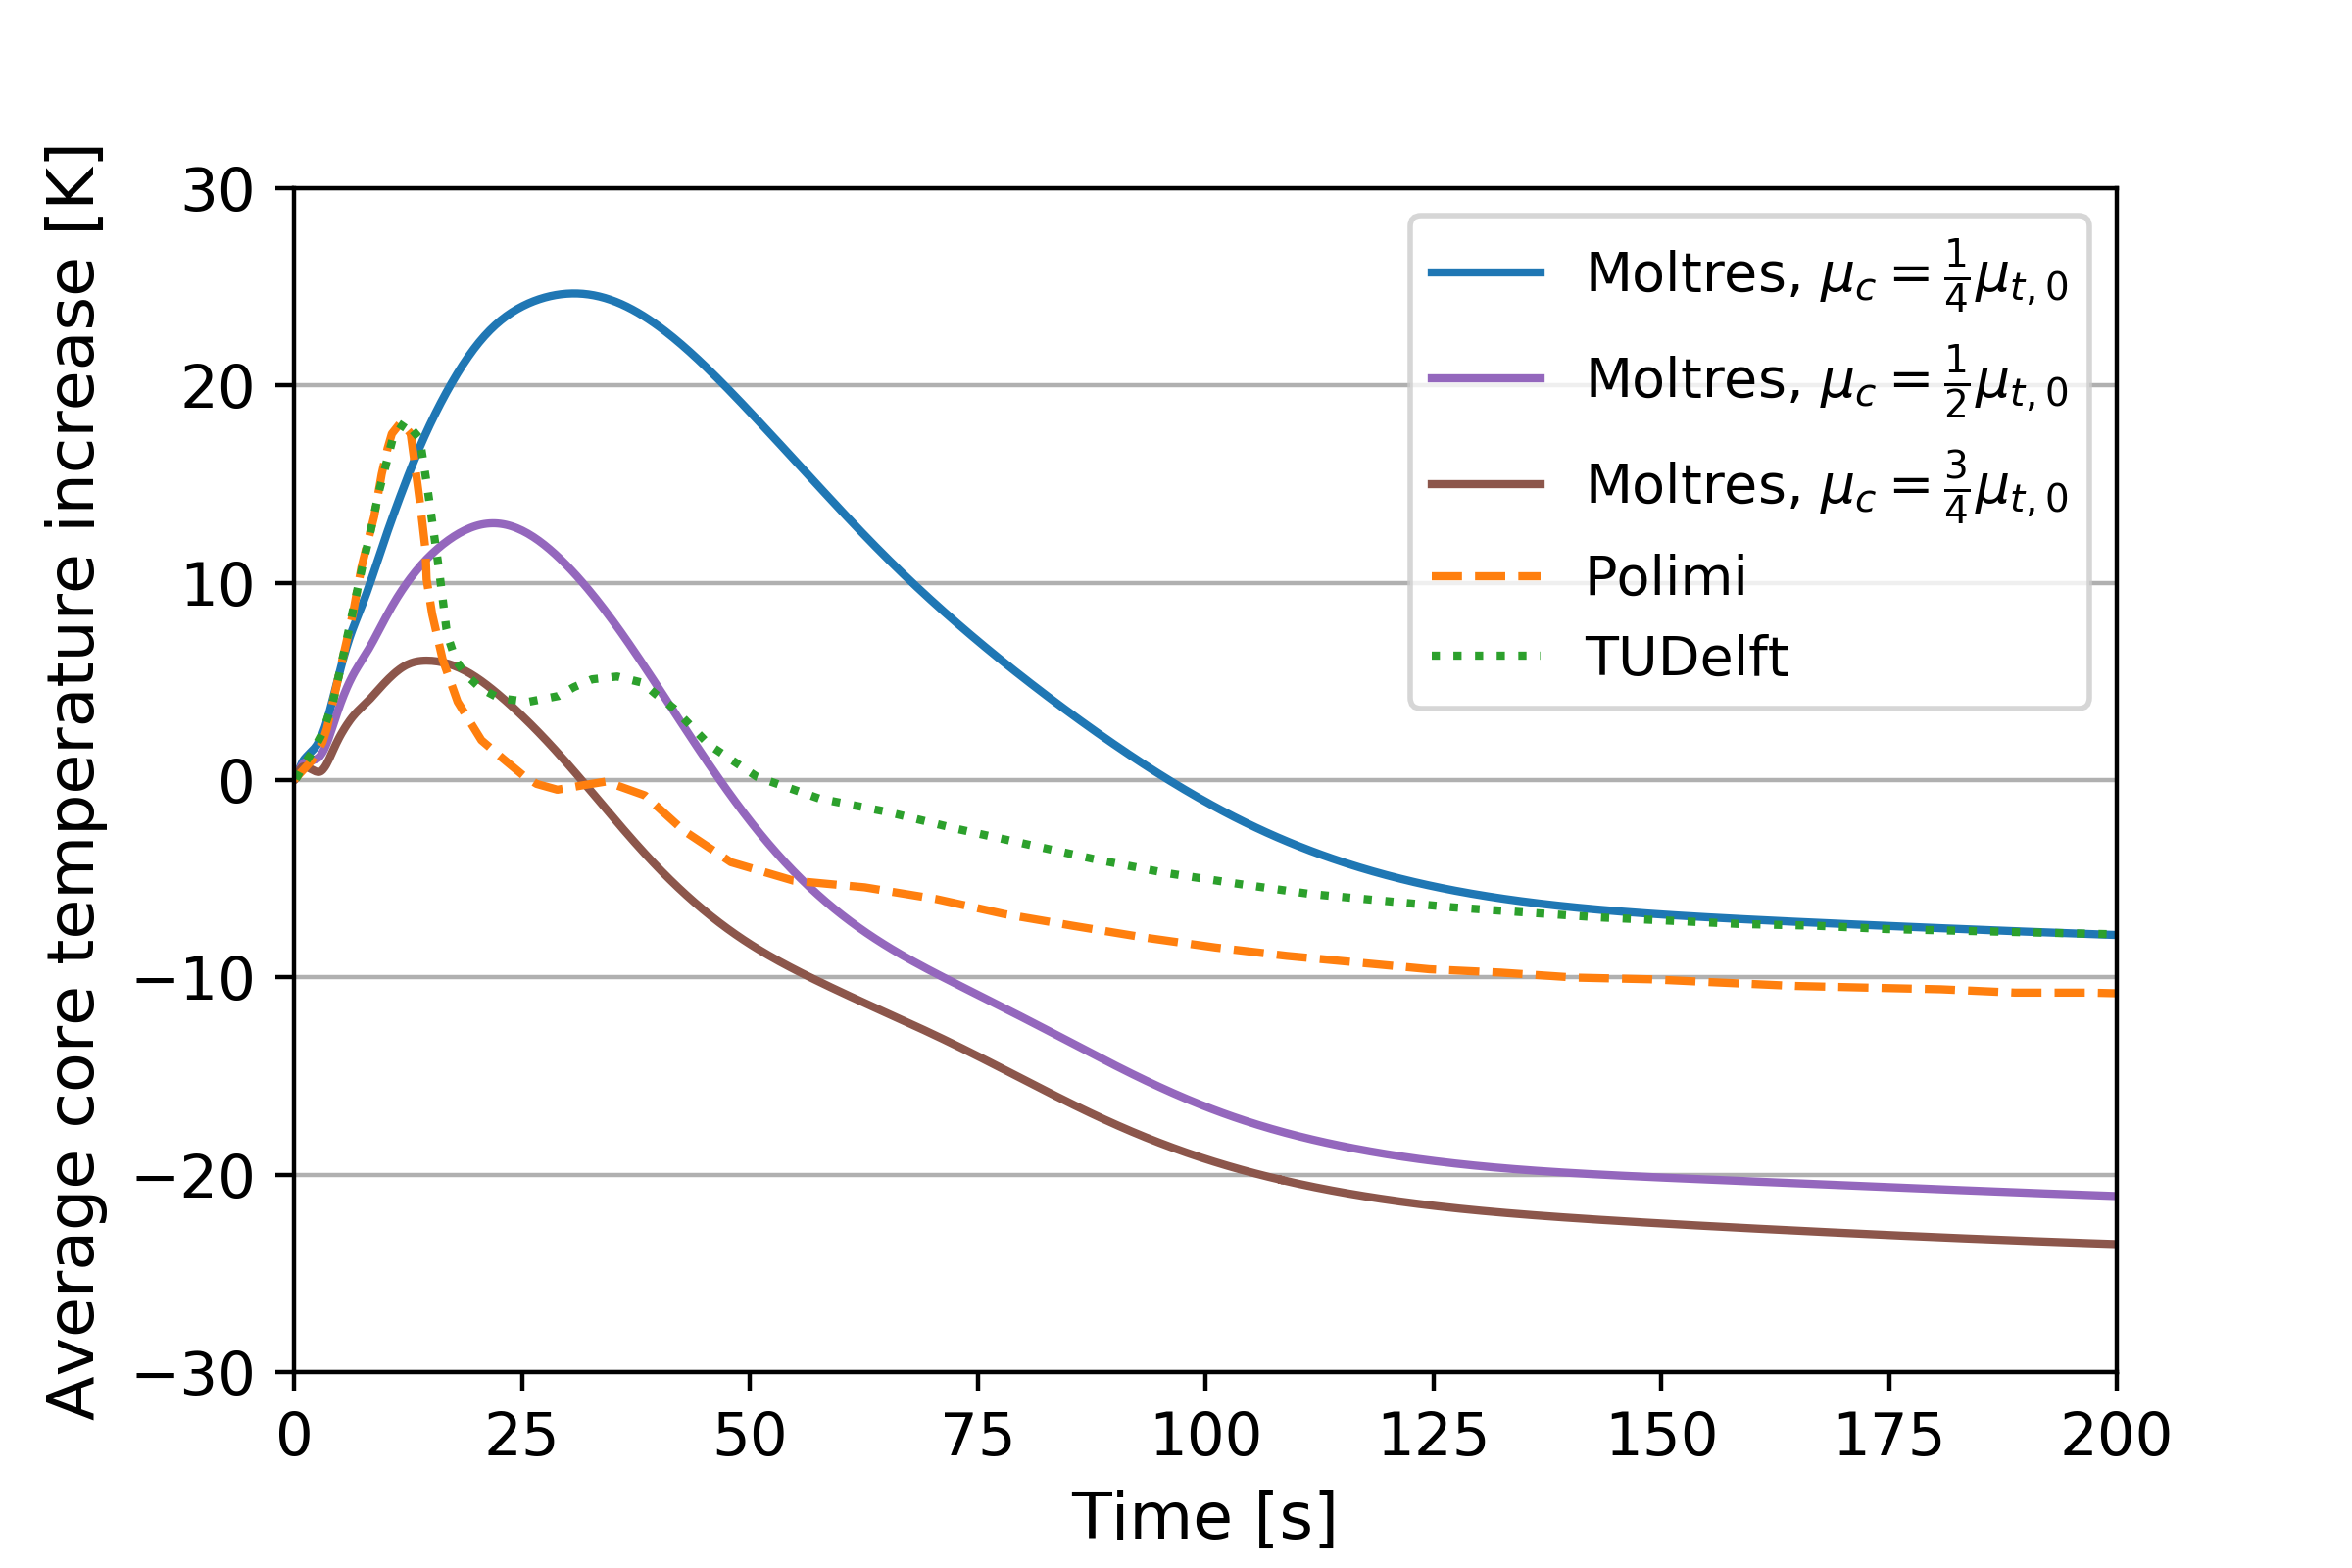
\includegraphics[width=.85\textwidth]{lof-temp}
    \caption{Average core temperature increase during
    an unprotected loss of flow transient in the Moltres, Polimi, and
    TUDelft models \cite{fiorina_modelling_2014}.}
    \label{fig:loftemp}
\end{figure}

\begin{figure}[htbp!]
    \centering
    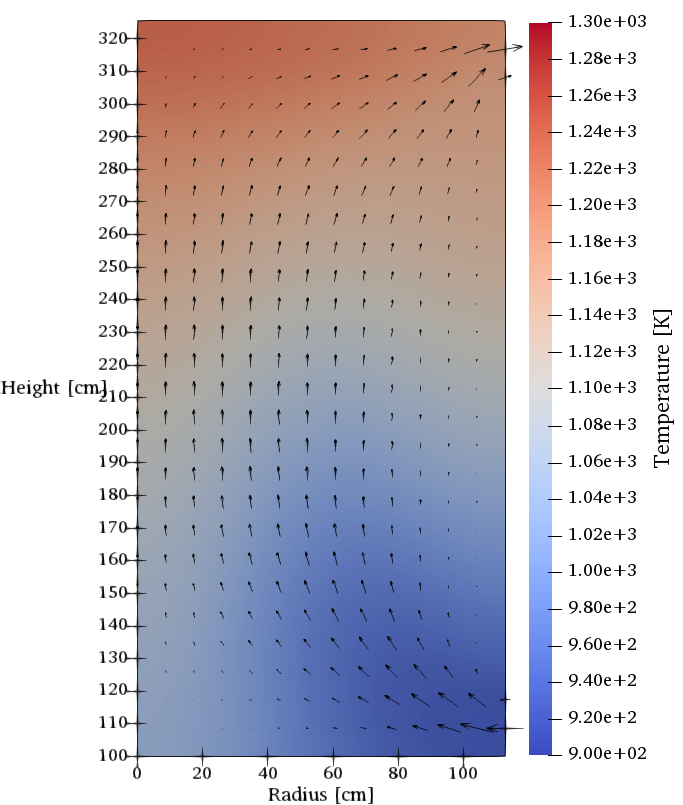
\includegraphics[width=.37\textwidth]{lof-flow-temp}
    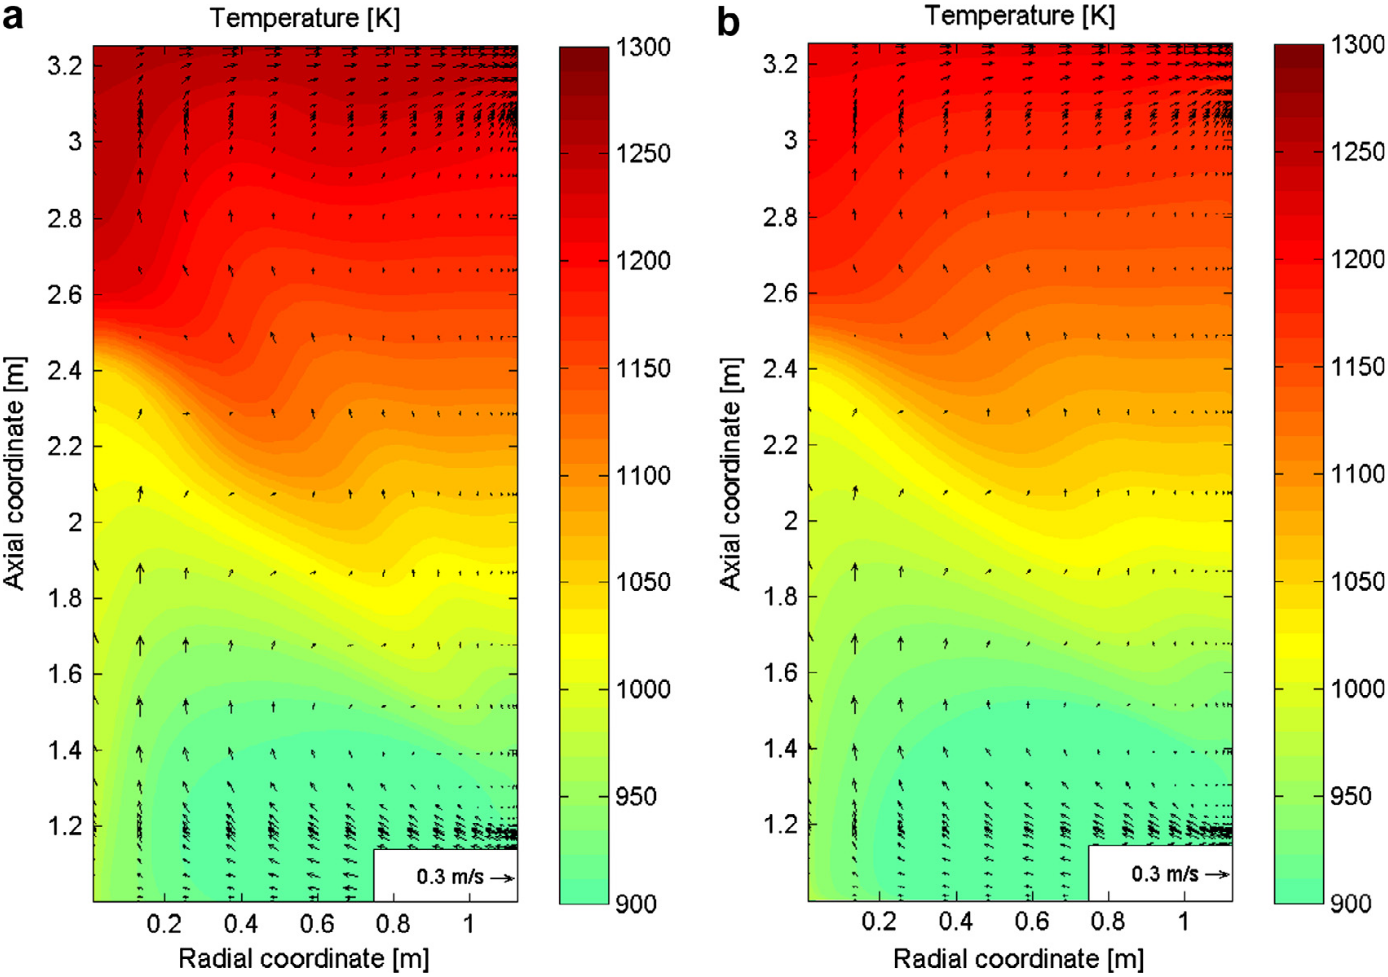
\includegraphics[width=.62\textwidth]{fiorina-lof}
    \caption{Temperature and velocity fields in the core at $t=300$ s during
    a loss of flow transient in the Moltres ($\mu_c = \frac{1}{2} \mu_{t,0}$),
    Polimi, and TUDelft models.}
    \label{fig:lofflowtemp}
\end{figure}

Figure \ref{fig:lofflowtemp} shows the flow patterns and temperature
distribution in the core at $t=300$ s in all three models. Figures
\ref{fig:lofheat}, \ref{fig:loftemp}, and \ref{fig:lofflowtemp} combined
highlight the difference between laminar flow in the Moltres model and
buoyancy-driven flow in the other models, and its impact on the reactor
response. They show that low-speed laminar flow is a poor substitute for
buoyancy-driven flow in the context of the MSFR. It is particularly evident
in the transition from high-speed turbulent flow to low-speed viscous
flow as Moltres mispredicted the intermediate stages. The
simplifying assumption for the uniform, time-dependent $\mu_t$ is also flawed
in a safety analysis code.

The results from this transient inform our goals for Moltres: 1)
implementing a proper turbulence model, and
2) developing a new heat exchanger feature that is compatible with the
buoyancy-driven flow capabilities already present in Moltres.

\clearpage

\section{Unprotected Pump Overspeed}

Pump overspeed refers to a sustained
increase in pump speed in the primary coolant loop. The increased flow rate
$\dot{m}$ impacts reactor performance in several ways.
It affects the neutronics by reducing the in-core $\beta$ as more of the
shorter-lived precursors will tend to flow out of the core before decaying.
This net loss of neutrons reduces the reactivity in the core, thereby causing
core temperatures to fall to counteract this change through temperature
reactivity feedback. The increased $\dot{m}$ also enhances the heat transfer
coefficient on the primary loop side of the heat exchanger and enables the
reactor to operate at a higher power output. At the same time, the improved
mixing flattens the temperature distribution in the core.

This workfollowed Fiorina et al.'s implementation
\cite{fiorina_modelling_2014} by
ramping up the inlet velocity, $u$, by 50\% from the nominal value, $u_0$,
according to the following formula:
%
\begin{align}
    u(t) &= u_0 [1 + 0.5 (1 - e^{-t / \tau})] \label{eq:overspeed}
    \intertext{where}
    \tau &= 5 \text{ s.} \nonumber
\end{align}
%
For this transient, this work assumed that $\mu_t$ was directly proportional
to $v$ because the buoyancy effects are negligible and the recirculation zones 
persist throughout the entire duration. Figures \ref{fig:poheat} and
\ref{fig:potemp} show the power output and average core temperature increase
during the unprotected pump overspeed transient in the Moltres, Polimi, and
TUDelft models. Figure \ref{fig:poshort} shows the same results for the first
20 seconds of the transient. At the start of the transient, the rising flow
rate cools the core and causes power output to rise sharply. Although the
average core temperature has a strictly decreasing trend, the temperature at
the center of the core briefly rises due ot the sharp increase in power
output. Since this is the region where most of the fissions take place, the
Doppler effect and salt expansion causes the power output to stall and dip
briefly before rising again at $t=2.5$ s. The reactor tends to a new
equilibrium power output and average core temperature. The temperature
distribution in the core is more evenly distributed because the turbulent
thermal conductivity $k_t$ is directly proportional to $mu_t$.

\begin{figure}[htbp!]
    \centering
    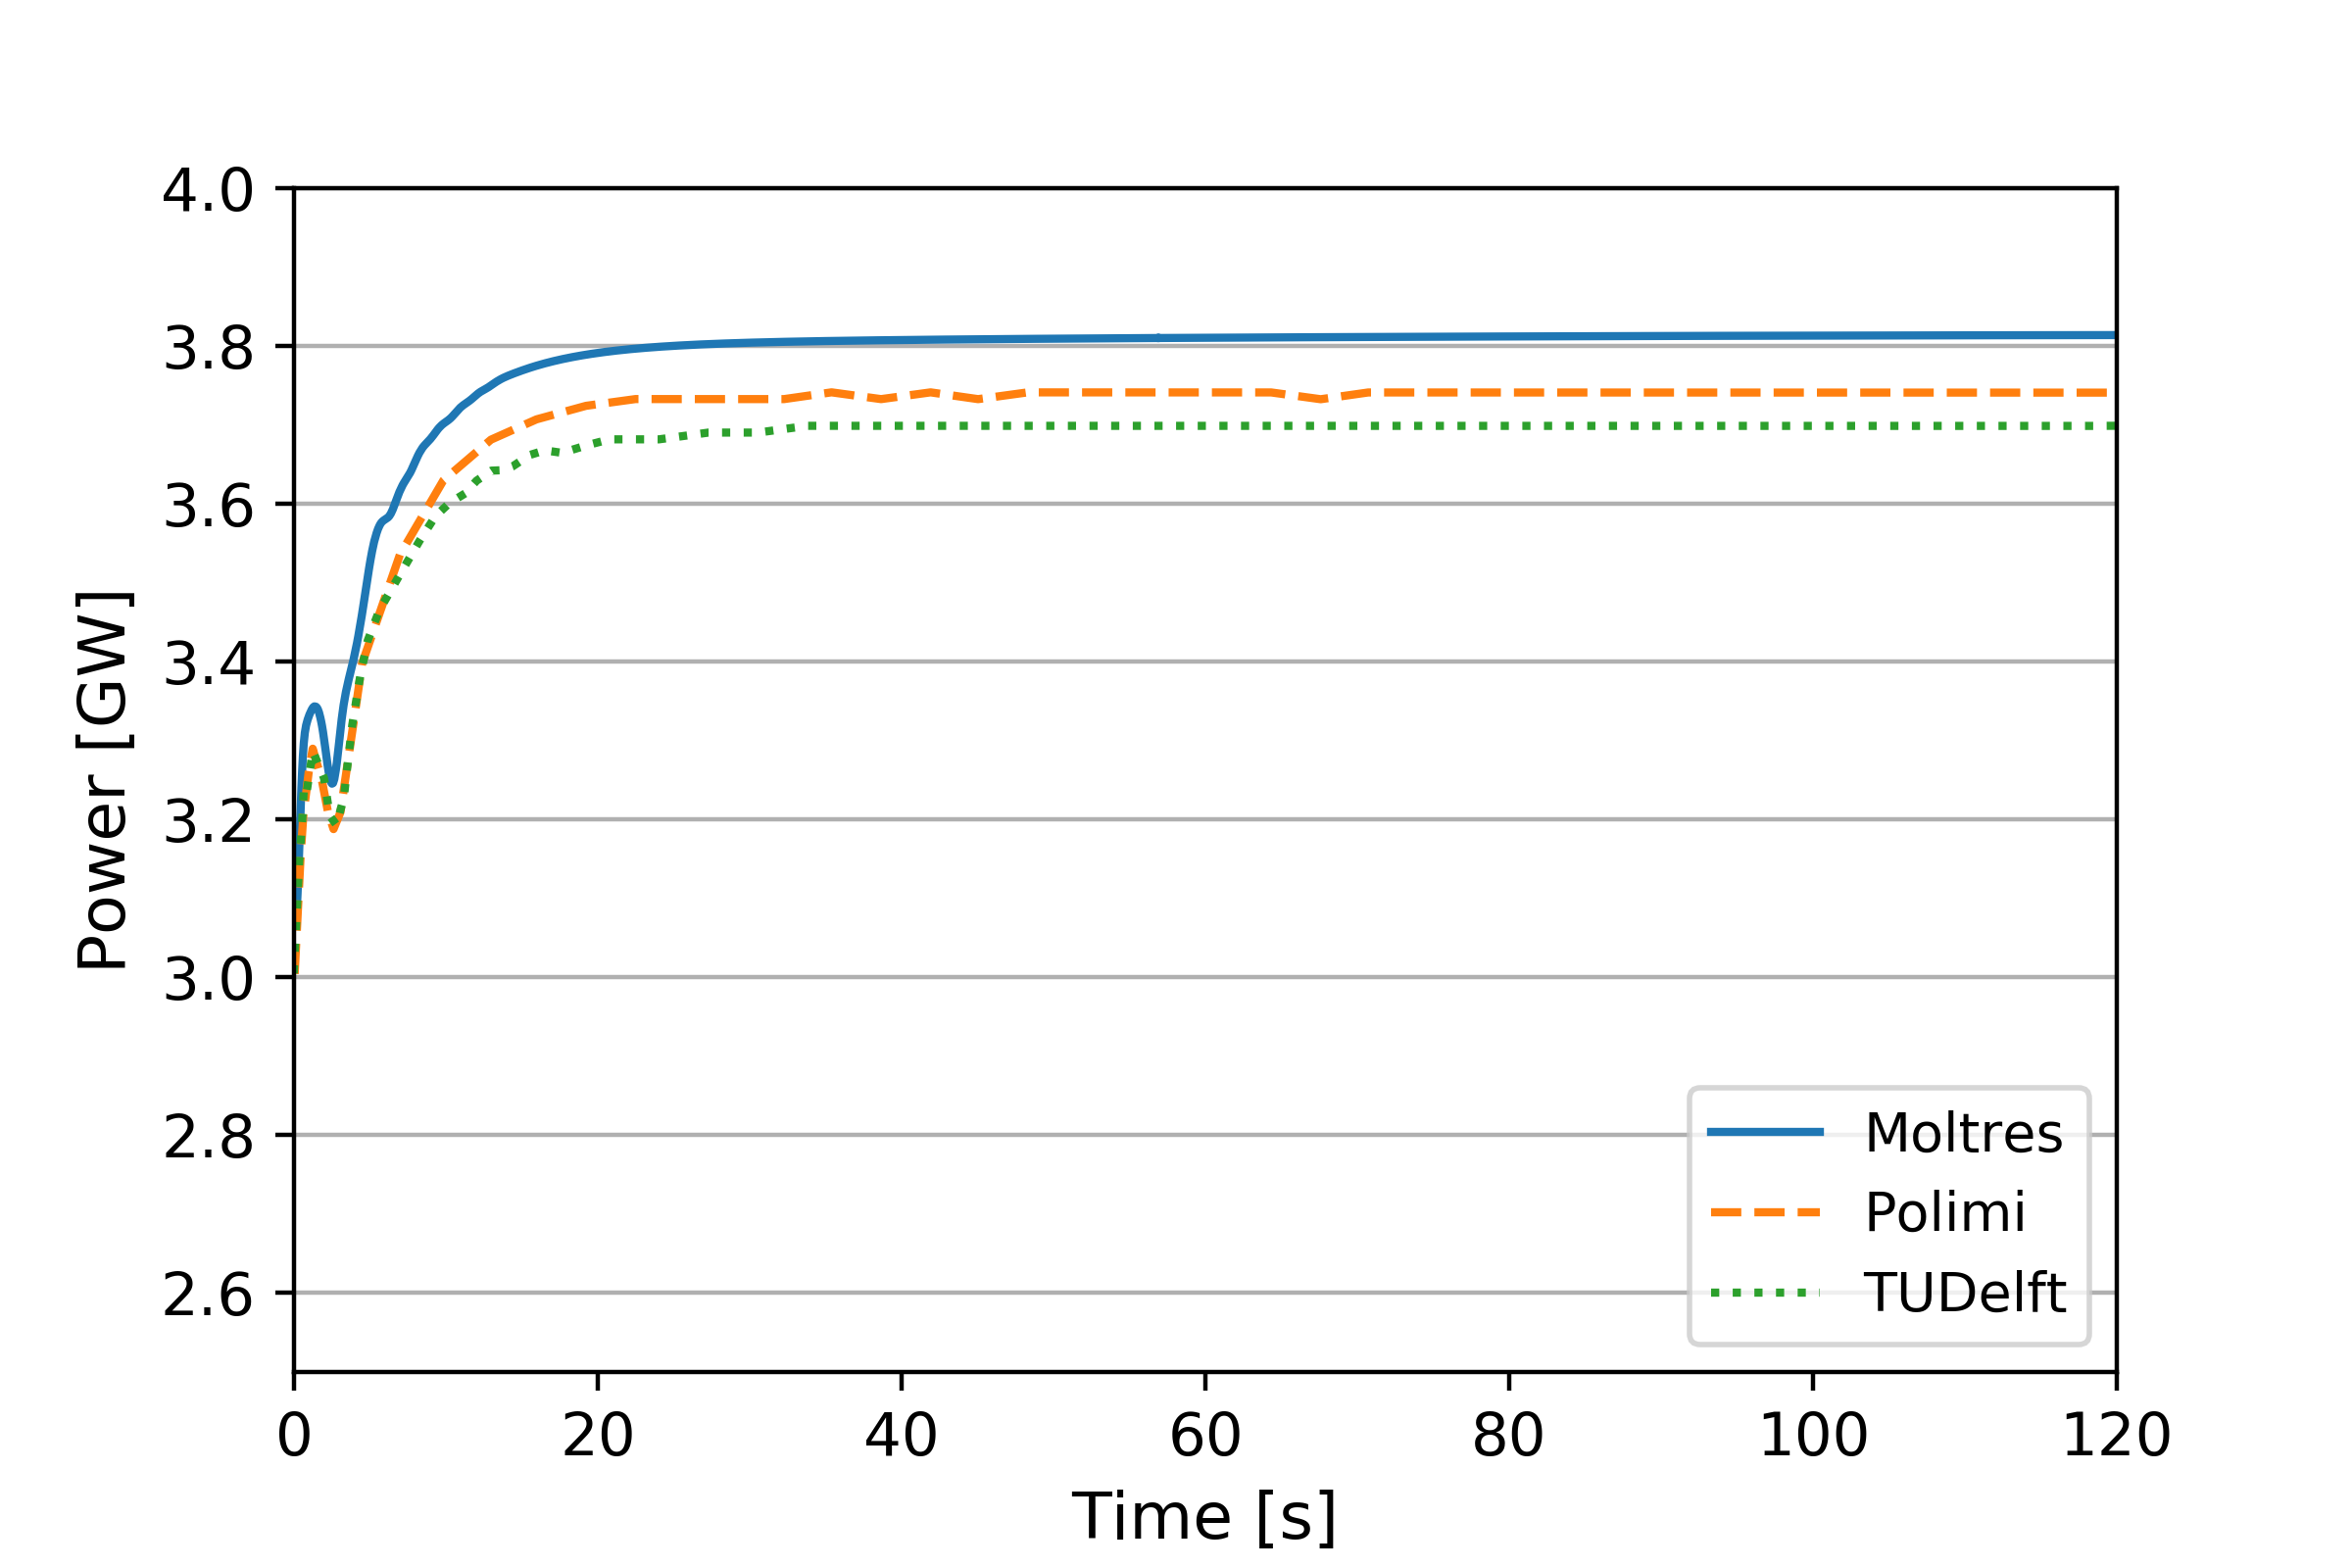
\includegraphics[width=.85\textwidth]{po-heat}
    \caption{Power output during
    an unprotected pump overspeed transient in the Moltres, Polimi, and
    TUDelft models \cite{fiorina_modelling_2014}.}
    \label{fig:poheat}
    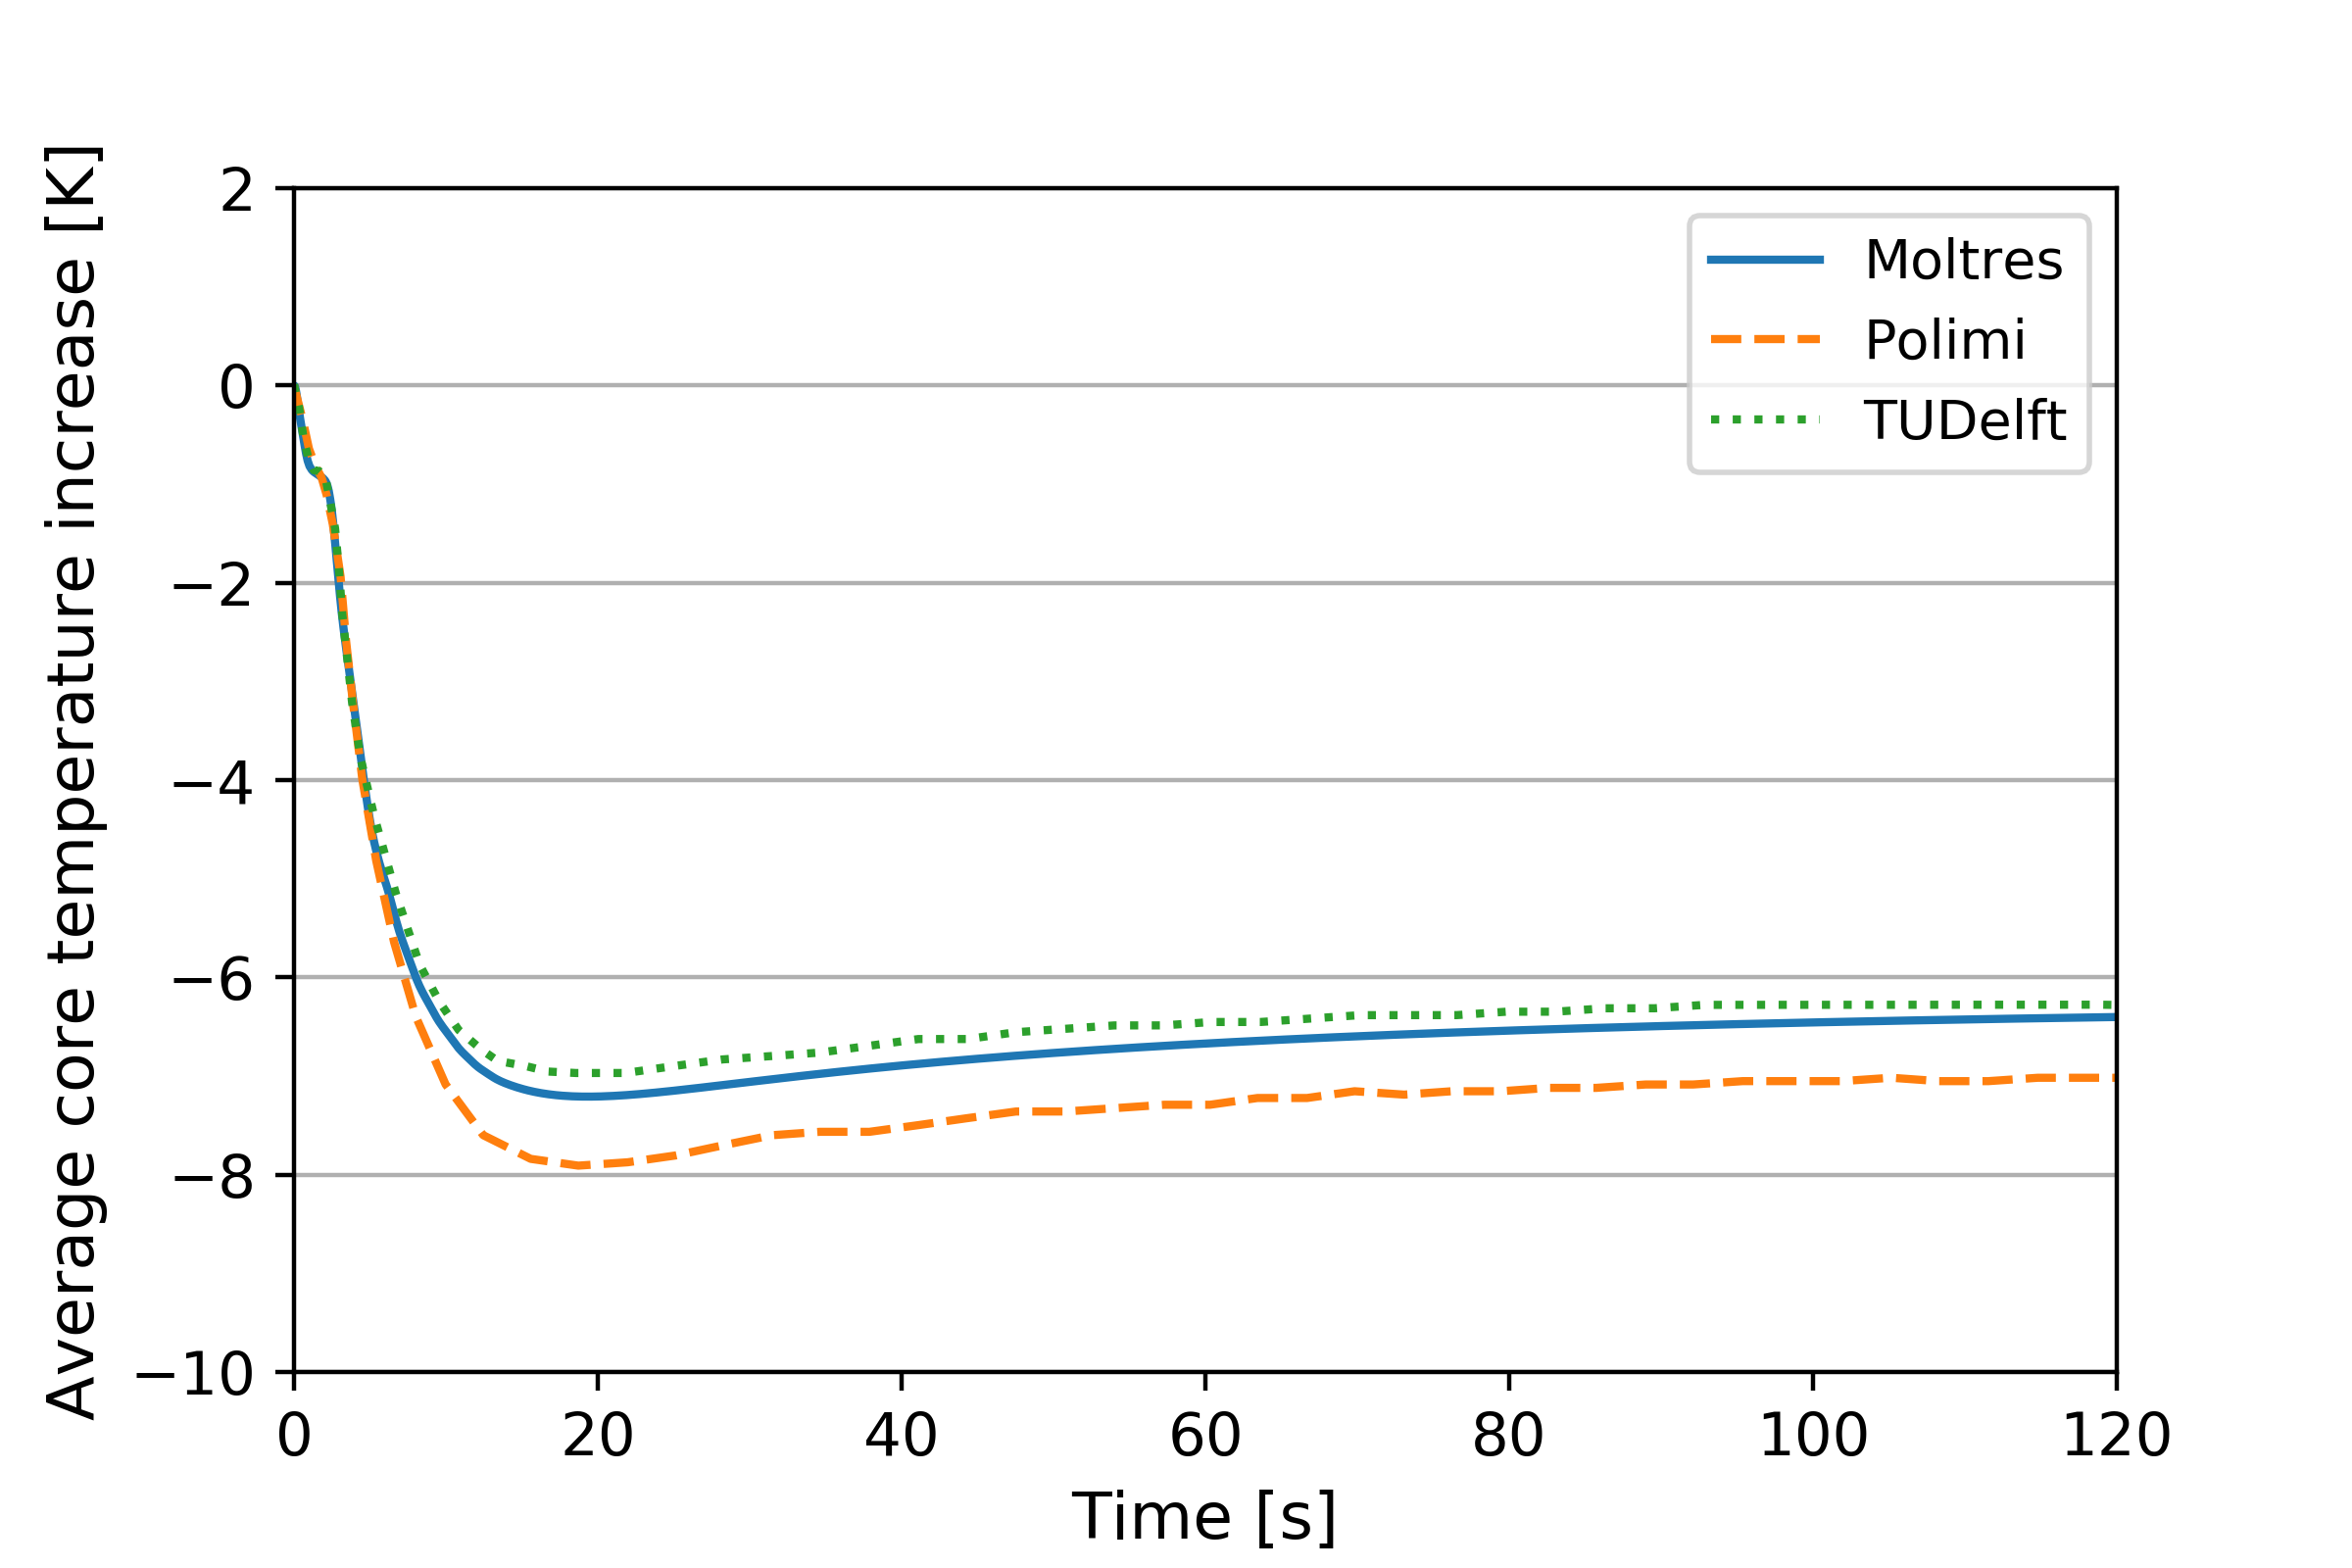
\includegraphics[width=.85\textwidth]{po-temp}
    \caption{Average core temperature increase during
    an unprotected pump overspeed transient in the Moltres, Polimi, and
    TUDelft models \cite{fiorina_modelling_2014}.}
    \label{fig:potemp}
\end{figure}

\begin{figure}[htbp!]
    \centering
    \begin{subfigure}[t]{.485\textwidth}
        \centering
        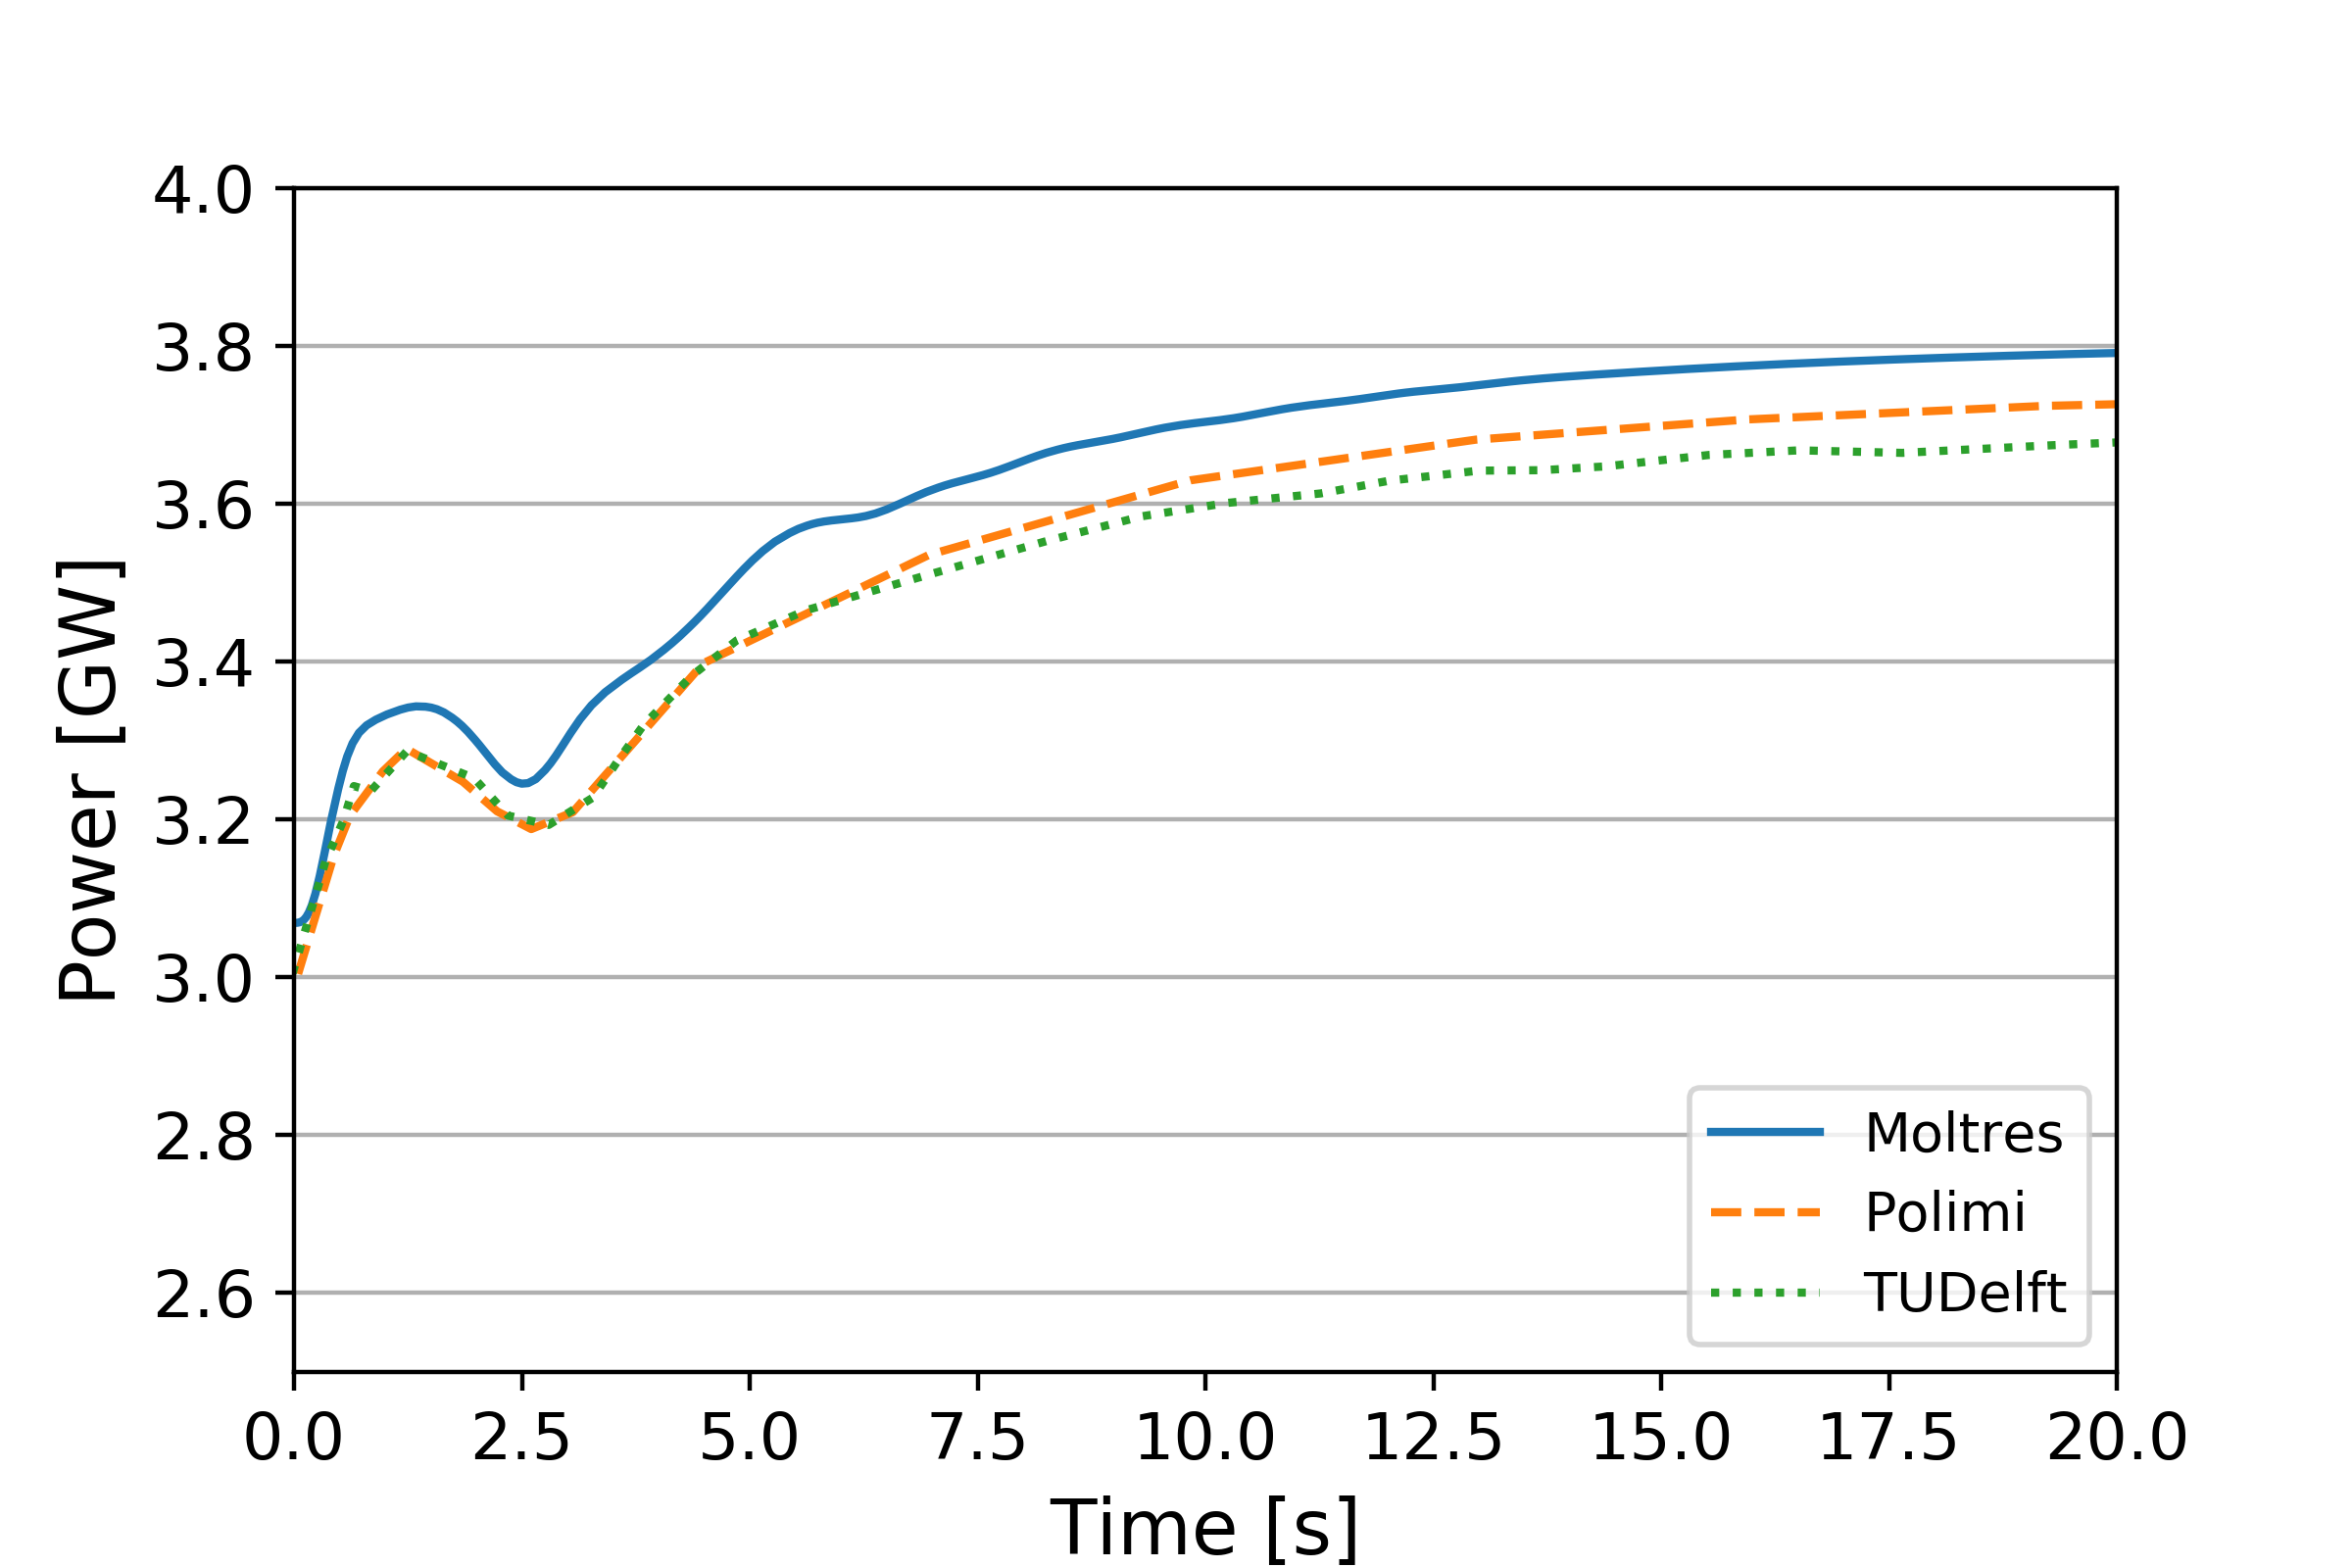
\includegraphics[width=\textwidth]{po-heat-short}
    \end{subfigure}
    \hfill
    \begin{subfigure}[t]{.485\textwidth}
        \centering
        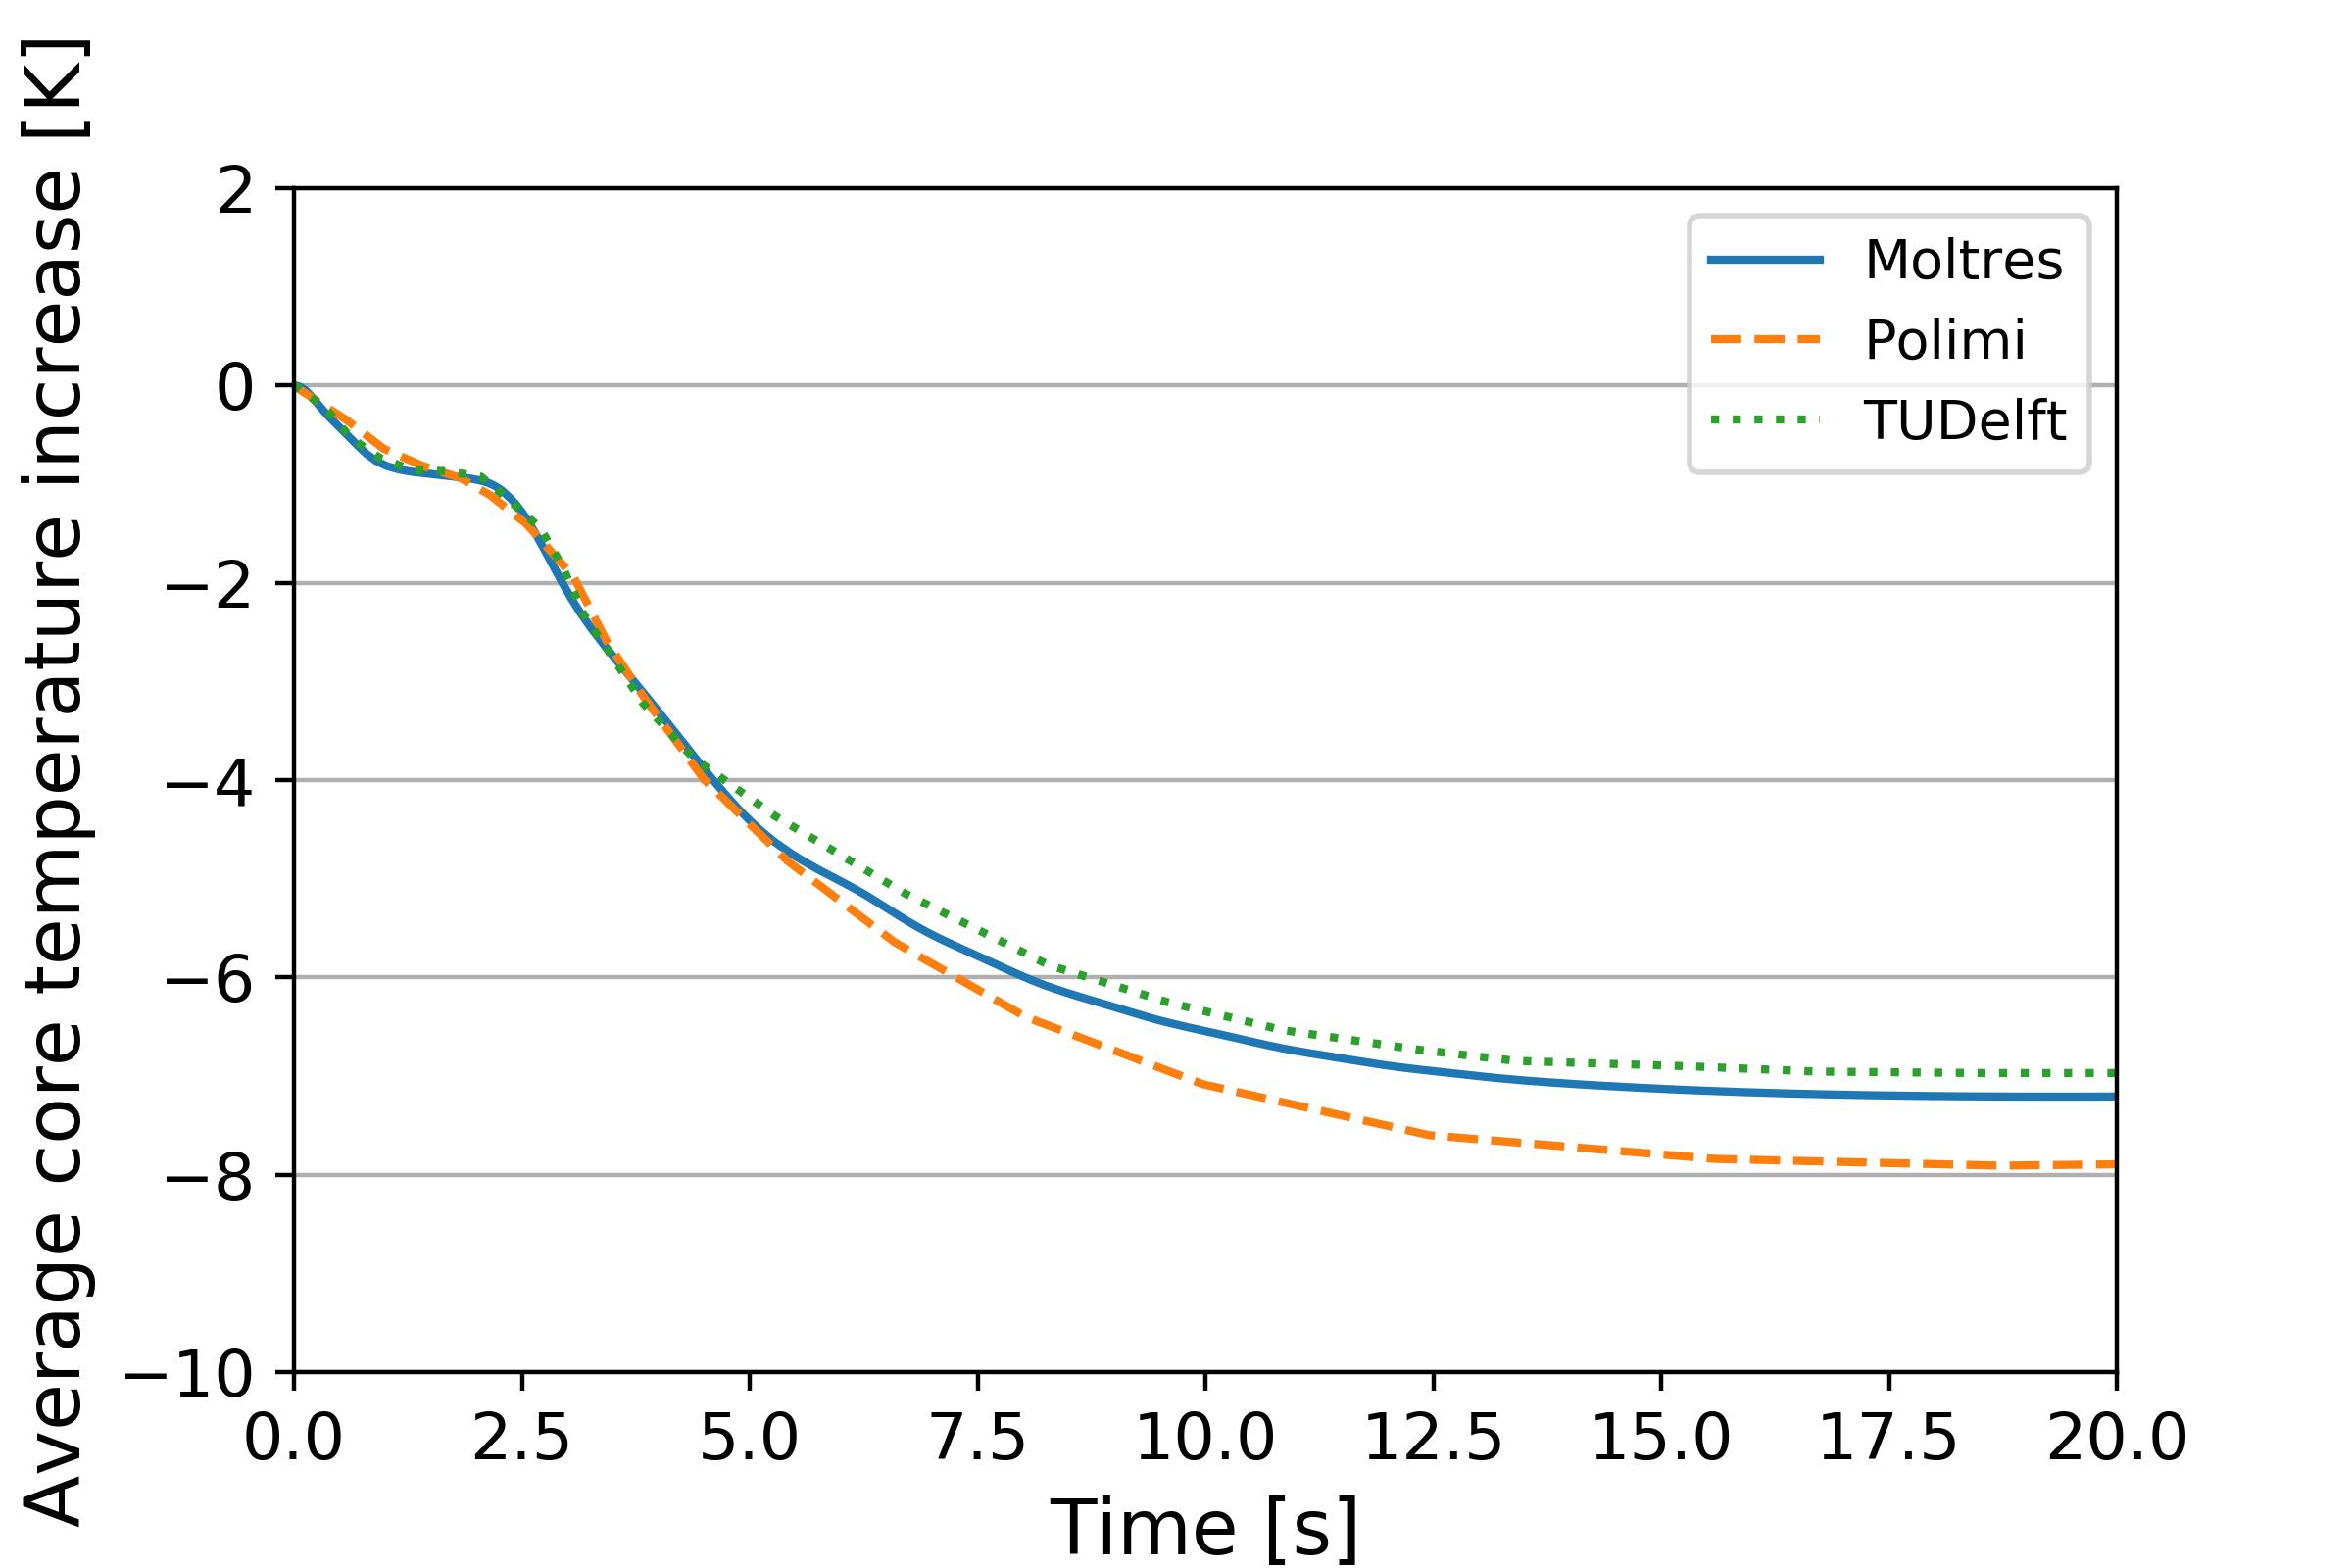
\includegraphics[width=\textwidth]{po-temp-short}
    \end{subfigure}
    \caption{The first 20 s of the power output and average core temperature
    increase during an unprotected pump overspeed transient.}
    \label{fig:poshort}
\end{figure}

The results show excellent agreement with the Polimi and TUDelft models. The
average core temperature increase in particular reproduces the Polimi and   
TUDelft results very well and the curve falls between the other two curves.
The power output is higher because the Moltres \gls{MSFR} model has a
stronger negative temperature coefficient than the other two models. 


%\chapter{Conclusion}
%%The unique phenomena in \glspl{MSR}, generally not found in conventional
reactors, necessitate the development of new reactor safety analysis software.
This thesis presents the latest developments in Moltres, namely coupling its
existing neutron diffusion module to the incompressible Navier-Stokes module
in MOOSE, and developing a decay heat model for short-term transients. We
demonstrated and verified some of its current capabilities through a static
neutronics study, and a coupled neutronics/thermal-hydraulics safety analysis
of the \gls{MSFR} concept.

The neutronics study showed good agreement between Moltres and Serpent. With
the relevant group constant data from Serpent,
Moltres could accurately replicate the $k_{eff}$, $\beta$,
$\alpha_T$, and multi-group neutron flux results from Serpent. The
$k_{eff}$ estimates from Moltres were approximately 100 pcm higher for all
measurements between 800 K and 1400 K. This discrepancy is notably smaller
than the discrepancies observed in the neutron diffusion and SP3 models
developed in OpenFOAM \cite{aufiero_extended_2013}. The $\beta$ and $\alpha_T$
values from Moltres had 1.46\% and 0.265\% discrepancies, respectively, to
Serpent's results. Lastly, the normalized six-group neutron flux from Moltres
and Serpent were visually indistinguishable from each other. The journal
article that introduced Moltres \cite{lindsay_introduction_2018} verified its
neutron diffusion model for a two-group thermal-spectrum \gls{MSBR} model;
the results of this study extends code-to-code verification of Moltres'
neutron diffusion model with the six-group, fast-spectrum \gls{MSFR} model.

Although Moltres currently lacks a proper turbulence model, our simplifying
assumption for the turbulent viscosity $\mu_t$ yielded good results for most
of the \gls{MSFR}
steady-state and transient analyses. The steady-state temperature and velocity
distributions showed many similiarities in their shapes and magnitudes to the
Polimi and TUDelft model results \cite{fiorina_modelling_2014}. Our
uniform $\mu_t$ assumption accounted for the minor differences in the flow at
the top of the core and the loss of delayed neutrons to out-of-core emissions.
The results with the decay heat model showed a slight flattening of the
temperature distribution in the core that is in line with our expectations
given the diffusion and advection of the decay heat precursors.

The unprotected reactivity insertion and loss of heat sink results showed the
same trends Fiorina et al. observed in their Polimi and TUDelft models. The
small difference in the temperature reactivity coefficient accounted for the
small difference in the magnitude of the peaks in power output and average
core temperature increase. The differences between the pointwise heat
exchanger in Moltres and the volumetric heat exchanger in the other two
models required minor adjustments in the relationship between flow rate
$\dot{m}$ and the heat transfer coefficient $h$ from the original
Dittus-Boelter correlation for the pump-initiated transients. Assuming a
directly proportional relationship between $\mu_t$ and $\dot{m}$ yielded
results in good agreement with the other two models for the pump overspeed
transient. However, Moltres performed poorly in the loss of flow transient as
we could not incorporate buoyancy-driven flow and its associated effects on
$\mu_t$.

Overall, we have demonstrated that Moltres can handle most of the case
studies that this thesis covered.

\section{Future Work}

Further research and development on Moltres should aim to rectify the issues
mentioned in this thesis. There are three main avenues for improvement.
Firstly, proper 2D/3D heat exchanger implementation
would allow us to move away from the 1D outer loop system and towards a full
2D/3D closed loop. The biggest change from this is users would be able to use
the Boussinesq approximation for buoyancy-driven flow capability in Moltres.
Buoyancy-driven flow is a critical component in loss of forced flow scenarios
and these scenarios in turn are important accident transients in reactor
safety analyses.

Secondly, Moltres would benefit from a proper turbulence model such as the
$k$-$\epsilon$ or $k$-$\omega$ turbulence models. Turbulence effects are
significant in \gls{MSR} designs with fast flow, and they inform optimization
studies for improving flow patterns and eliminating local hotspots in eddies.
Our work in this thesis, particularly for the loss of flow transient, shows
that simplifying assumptions for turbulence lead to erroneous results under
flow conditions that deviate significantly from steady state.

Lastly, a compressible Navier-Stokes model would be essential for modeling
compressible flow effects such as variable temperature-dependent density
changes following a large reactivity insertion and finite wave propagation
speeds in a fluid. The presence of bubbles in the core from the gas sparging
system increases fuel compressibility and enhances compressibility effects
\cite{cervi_development_2019}. 


%\chapter*{Appendix}
%Appendix.

\backmatter

\bibliographystyle{ieeetr}
\bibliography{bibliography}

\end{document}
\endinput
%%
